%  article.tex (Version 3.3, released 19 January 2008)
%  Article to demonstrate format for SPIE Proceedings
%  Special instructions are included in this file after the
%  symbol %>>>>
%  Numerous commands are added out, but included to show how
%  to effect various options, e.g., to print page numbers, etc.
%  This LaTeX source file is composed for LaTeX2e.

%  The following commands have been added in the SPIE class
%  file (spie.cls) and will not be understood in other classes:
%  \supit{}, \authorinfo{}, \skiplinehalf, \keywords{}
%  The bibliography style file is called spiebib.bst,
%  which replaces the standard style unstr.bst.

%\documentclass[a4paper]{spie}
\documentclass[]{spie}  %>>> use for US letter paper
%%\documentclass[a4paper]{spie}  %>>> use this instead for A4 paper
%%\documentclass[nocompress]{spie}  %>>> to avoid compression of citations
%% \addtolength{\voffset}{9mm}   %>>> moves text field down
%% \renewcommand{\baselinestretch}{1.65}   %>>> 1.65 for double spacing, 1.25 for 1.5 spacing
%  The following command loads a graphics package to include images
%  in the document. It may be necessary to specify a DVI driver option,
%  e.g., [dvips], but that may be inappropriate for some LaTeX
%  installations.
\usepackage[]{graphicx}
\usepackage{color}
\usepackage{cancel}
\usepackage{amsmath}
\usepackage{amsfonts}
\usepackage{mathtools}
\usepackage{verbatim}
\usepackage{titlesec}
\definecolor{linkcolor}{cmyk}{1, 0.65, 0, 0.3}			% PANTONE 288 CVU
\definecolor{citecolor}{cmyk}{0.79, 0, 0.87, 0.56}		% PANTONE 357 CVU
%\definecolor{citecolor}{cmyk}{1, 0, 0.47, 0.3}			% PANTONE 328
\def\red{\textcolor{red}}
\def\blue{\textcolor{blue}}
\usepackage[
	colorlinks,
	linkcolor=linkcolor,
	urlcolor=linkcolor,
	citecolor=linkcolor,
	pdftex,
	pdfstartview=FitH,
]{hyperref}

\titleformat{\section}{\normalfont\fontsize{11.5pt}{1em}\bfseries}{SUPPLEMENTARY NOTE \thesection: }{0em}{}
\titleformat{\subsection}{\normalfont\fontsize{11pt}{0.75em}\bfseries}{SUPPLEMENTARY NOTE \thesubsection: }{0em}{}
\titleformat{\subsubsection}{\normalfont\fontsize{11pt}{0.75em}\bfseries}{SUPPLEMENTARY NOTE \thesubsubsection: }{0em}{}

% jump to the top of a figure, not the caption
\usepackage[all]{hypcap}

% so that footnotes in tables work
\usepackage{footnote}

% so that we can omit the 'Table 1:' for the overview
\usepackage{caption}

% should be called Supplementary Figure
\renewcommand{\figurename}{Supplementary Figure}

% for the source code
\usepackage{listings}

\usepackage{helvet}
\renewcommand{\rmdefault}{\sfdefault}
\renewcommand{\baselinestretch}{1.05}

%\usepackage{sectsty}Bayesian-based single-view and multi-view deconvolution
%\allsectionsfont{\sffamily}

\usepackage{pdflscape}
\usepackage{booktabs}
\usepackage{makecell}
\usepackage{longtable}
\usepackage{multirow}

\captionsetup[table]{labelformat=empty}

\newcommand\smallurl[1]{{\small{\url{#1}}}}
\newcommand\tablespace{\vspace{2.5mm}}
\newcommand\fig{supplementary figure }
\newcommand\Fig{Supplementary figure }


\title{BigStitcher: Reconstructing high-resolution image datasets of cleared and expanded samples}

%>>>> The author is responsible for formatting the
%  author list and their institutions.  Use  \skiplinehalf
%  to separate author list from addresses and between each address.
%  The correspondence between each author and his/her address
%  can be indicated with a superscript in italics,
%  which is easily obtained with \supit{}.

\author{David H{\"o}rl\textsuperscript{\#}, Fabio Rojas Rusak\textsuperscript{\#}, Friedrich Preusser, Paul Tillberg, Nadine Randel, Raghav~K.~Chhetri, Albert Cardona, Philipp J. Keller, Hartmann Harz, Heinrich Leonhardt, Mathias Treier, Stephan Preibisch\textsuperscript{*}
%\skiplinehalf
%\small{
%\supit{1}Max Planck Institute of Molecular Cell Biology and Genetics, Pfotenhauerstrasse 108, Dresden, Germany \\
%\supit{2}HHMI Janelia Farm Research Campus, 19700 Helix Drive, Ashburn, VA 20147, USA \\
%\supit{3}Albert Einstein College of Medicine, 1300 Morris Park Avenue, Bronx, NY 10461, USA
%}
}

%>>>> Further information about the authors, other than their
%  institution and addresses, should be included as a footnote,
%  which is facilitated by the \authorinfo{} command.

%\authorinfo{Further author information: (Send correspondence to A.A.A.)\\A.A.A.: E-mail: aaa@tbk2.edu, Telephone: 1 505 123 1234\\  B.B.A.: E-mail: bba@cmp.com, Telephone: +33 (0)1 98 76 54 32}
%%>>>> when using amstex, you need to use @@ instead of @


%%%%%%%%%%%%%%%%%%%%%%%%%%%%%%%%%%%%%%%%%%%%%%%%%%%%%%%%%%%%%
%>>>> uncomment following for page numbers
\pagestyle{plain}
%>>>> uncomment following to start page numbering at 301
%\setcounter{page}{1}

% underset argument for (arg)max/min
\DeclareMathOperator*{\argmax}{arg\,max}
\DeclareMathOperator*{\argmin}{arg\,min}
%\DeclareMathOperator*{\max}{max}
%\DeclareMathOperator*{\min}{min}
%\DeclareMathOperator{\deg}{deg}

\begin{document}

\maketitle

%\pagestyle{headings}
\setcounter{page}{1}
\pagenumbering{roman}
\pagenumbering{arabic}


\hspace{5mm}

\begin{table}[h!]
\center
{
\fontsize{12pt}{11pt}\selectfont
\center
\begin{tabular}{lp{11cm}}
\textbf{\textcolor{red}{Supplementary File}} & \textbf{\textcolor{red}{Title}}\\ \\
\hline
\\
\textbf{\red{Supplementary Figure \ref{fig:sup-fig-rf}}} & \red{Quantification of fluorescence preservation in cleared tissue}\tablespace \\
\textbf{\red{Supplementary Figure \ref{fig:sup-fig-illu-select}}} & \red{Quantification of automatic illumination selection} \tablespace \\
\textbf{\red{Supplementary Figure \ref{fig:sup-chromatic}}} & \red{Chromatic aberration correction}\tablespace \\
\textbf{\red{Supplementary Figure \ref{fig:sup-spherical}}} & \red{Spherical aberration correction}\tablespace \\
\textbf{Supplementary Figure \ref{fig:sup-fig-manual-align1}} &  Manual alignment \tablespace \\
\textbf{Supplementary Figure \ref{fig:sup-fig-flatfield}} & Flat-field correction \tablespace \\
\textbf{\red{Supplementary Figure \ref{fig:sup-rFRC}}} & \red{Automatic quantification of image quality}\tablespace \\
\textbf{\red{Supplementary Figure \ref{fig:sup-rfrc-brain}}} & \red{Quality Estimation in whole-brain mouse acquisition}\tablespace \\
\textbf{Supplementary Figure \ref{fig:sup-fig-icp}} & Affine refinement via ICP \tablespace \\
\textbf{Supplementary Figure \ref{fig:sup-fig-globalopt}} & Global optimization \tablespace \\
\textbf{Supplementary Figure \ref{fig:sup-fig-stitching}} & Pairwise registration by phase correlation \tablespace \\
\textbf{Supplementary Figure \ref{fig:sup-fig-downsampling}} & Downsampling with different SNR \tablespace \\
\textbf{Supplementary Figure \ref{fig:sup-fig-downsampling-statistics-0}} & Downsampling error statistics 1 \tablespace \\
\textbf{Supplementary Figure \ref{fig:sup-fig-downsampling-statistics-1}} & Downsampling error statistics 2 \tablespace \\
\textbf{Supplementary Figure \ref{fig:sup-fig-downsampling-statistics-2}} & Downsampling error statistics 3 \tablespace \\
\textbf{Supplementary Figure \ref{fig:sup-fig-link-explorer}} & Interactive inspection and curation of pairwise links \tablespace \\
\textbf{\red{Supplementary Figure \ref{fig:sup-fig-registration-quality}}} & \red{Quantification of image registration quality}\tablespace \\
\textbf{Supplementary Figure \ref{fig:sup-fig-boundingbox}} & Bounding-box definition \tablespace \\
\textbf{Supplementary Figure \ref{fig:sup-fig-fusion}} & Virtual fusion of large image \tablespace \\
\textbf{Supplementary Figure \ref{fig:sup-fig-interest-point}} & Interest point visualization \tablespace \\
\textbf{Supplementary Figure \ref{fig:sup-fig-manual-align2}} & Manual transformation of multi-view datasets \tablespace \\
\textbf{Supplementary Figure \ref{fig:sup-fig-expansion-microscopy}} & Expansion microscopy reconstruction \tablespace \\
\textbf{\red{Supplementary Figure \ref{fig:non-rigid}}} & \red{Principles of non-rigid alignment}\tablespace \\
\end{tabular}}
\hspace{10mm}
\caption{\emph{Continued on the following page}}
\end{table}

\begin{table}[h!]
\center
{
\fontsize{12pt}{11pt}\selectfont
\center
\begin{tabular}{lp{11cm}}
\textbf{\textcolor{red}{Supplementary File}} & \textbf{\textcolor{red}{Title}}\\ \\
\hline
\\
\textbf{\red{Supplementary Table \ref{tab:datasets}}} & \red{Datasets used in this publication} \tablespace \\
\textbf{\red{Supplementary Table \ref{tab:benchmarks}}} & \red{Performance comparison} \tablespace \\
\textbf{Supplementary Note \ref{sec:sup-note1}-\ref{sec:expansion}} & Supplementary methods \tablespace \\
\textbf{Supplementary Note \ref{sec:documentation}} & BigStitcher user guide \tablespace \\
\textbf{Supplementary Note \ref{sec:example}} & Example datasets for BigStitcher \tablespace \\
\textbf{Supplementary Note \ref{sec:currentcode}} & Links to the current source codes \tablespace \\
\textbf{\red{Supplementary Note \ref{sec:bugs}}} & \red{Bug reports and feature requests} \tablespace \\

\end{tabular}}
\caption{\emph{Note: Supplementary Videos 1--\red{9} are available for download on the journal homepage.}}
\end{table}

~
\pagebreak

\titleformat{\section}{\centering\normalfont\fontsize{13.5pt}{1em}\bfseries}{SUPPLEMENTARY NOTE \thesection: }{0em}{}
\section*{SUPPLEMENTARY FIGURES}
\titleformat{\section}{\normalfont\fontsize{11.5pt}{1em}\bfseries}{SUPPLEMENTARY NOTE \thesection: }{0em}{}


\subsection*{\red{SUPPLEMENTARY FIGURE 1: Quantification of fluorescence preservation in cleared tissue}}
\vspace{-3mm}
\begin{figure*}[ht!]
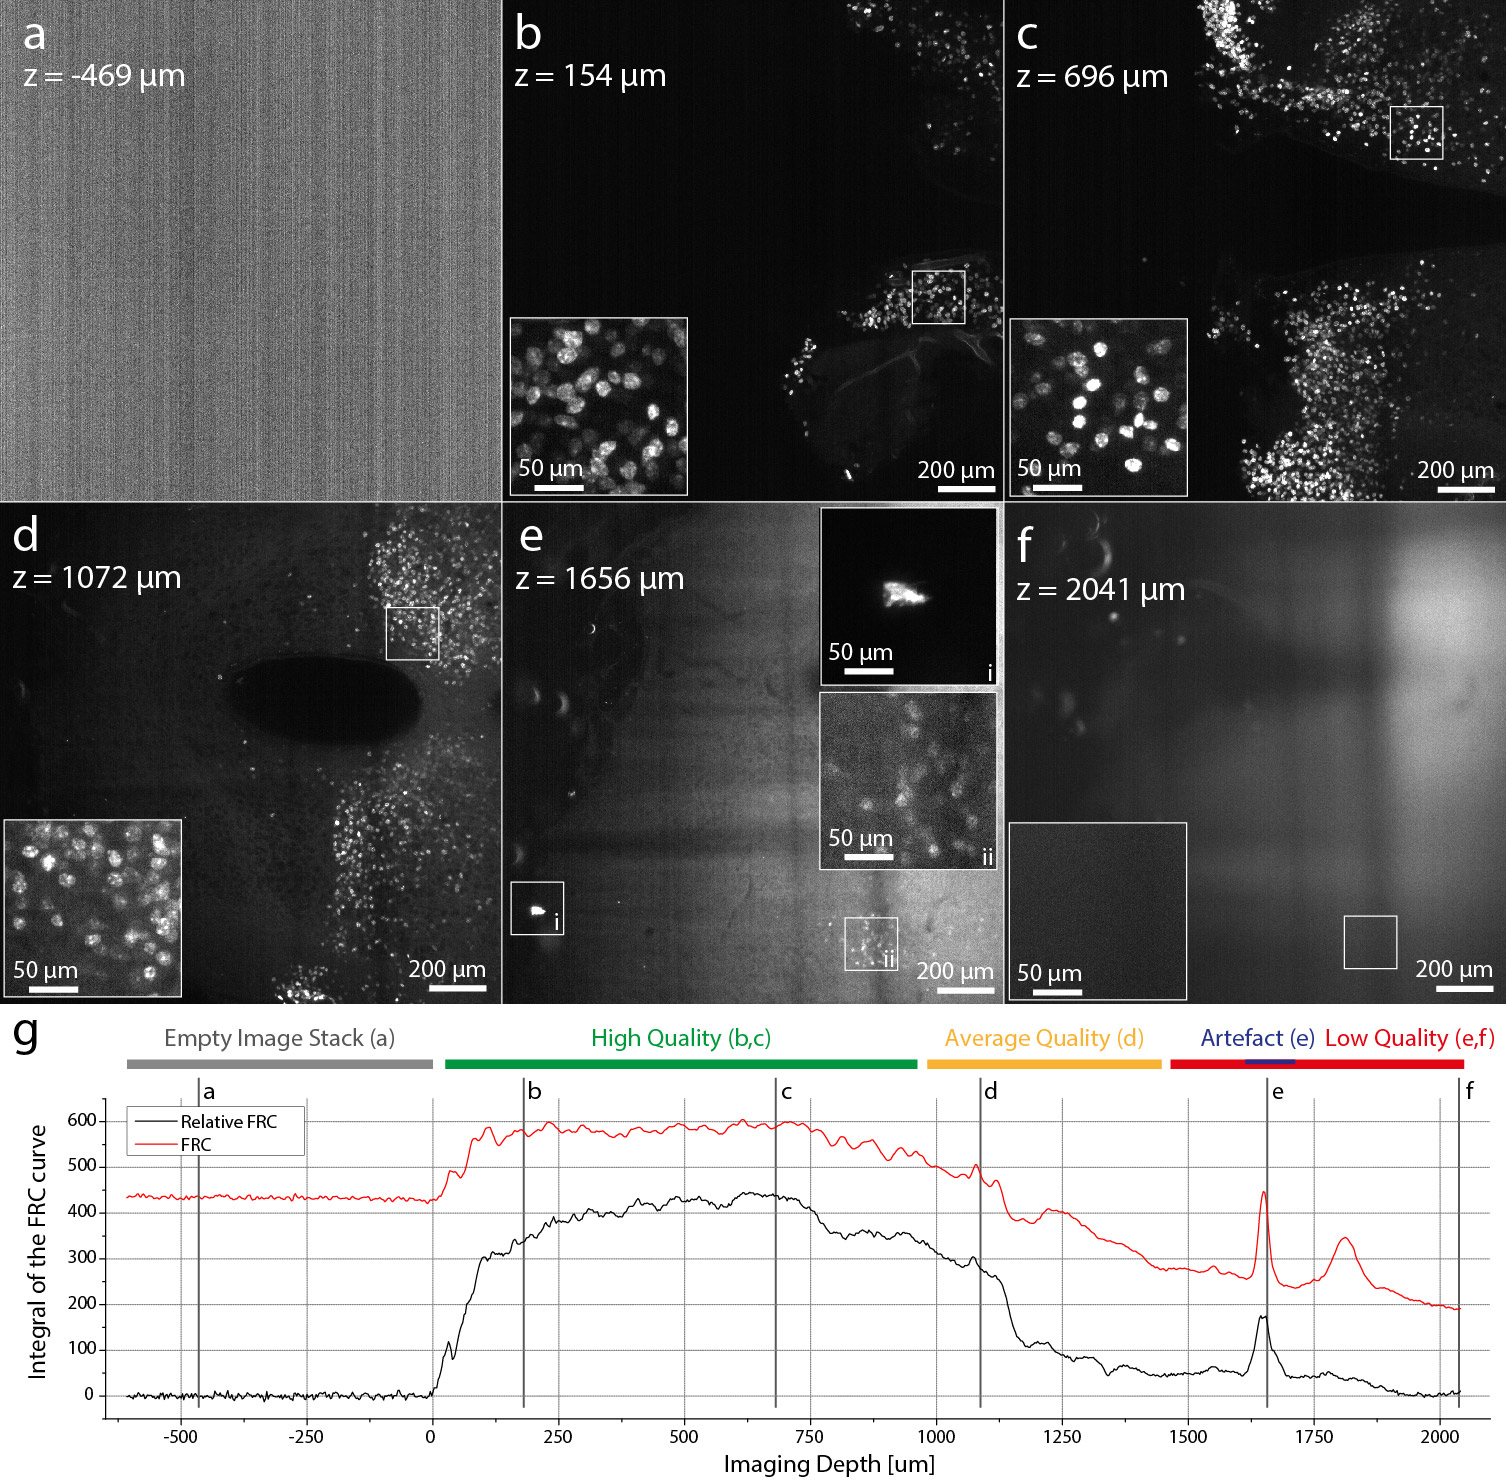
\includegraphics[width=\textwidth]{fig-rf.jpg}
\vspace{-4.0mm}
\caption{\hspace{-0.5mm}\red{\emph{Quantification of fluorescence preservation in cleared tissue.} \textbf{(a-f)} Optical sections through an CLARITY-cleared adult mouse hypothalamus expressing H2B-GFP in all bsx neurons. Fluorescence is preserved throughout the clearing procedure. However, the signal is degrading with imaging depth and can typically be recorded up to 1 -- 2 cm into the sample, depending on the tissue type and the quality of the clearing process limiting the size of the sample that can be acquired from a single orientation. Brightness and contrast was adjusted individually. \textbf{(g)} Quantification of image quality using (relative) Fourier Ring Correlation ([r]FRC, see \textbf{Online Methods}) in BigStitcher. Note that FRC produces high values for the camera patterns if no signal is present. The rFRC accurately measures image quality as illustrated by the position of the panels (a-f). As part of this publication similar experiments were performed 4$\times$ with comparable clearing results (\textbf{Fig. 1n, 3b, 3d}).} 
}
\label{fig:sup-fig-rf}
\end{figure*}

\pagebreak

\subsection*{\red{SUPPLEMENTARY FIGURE 2: Quantification of automatic illumination selection}}
\vspace{1mm}
\begin{figure*}[h!]
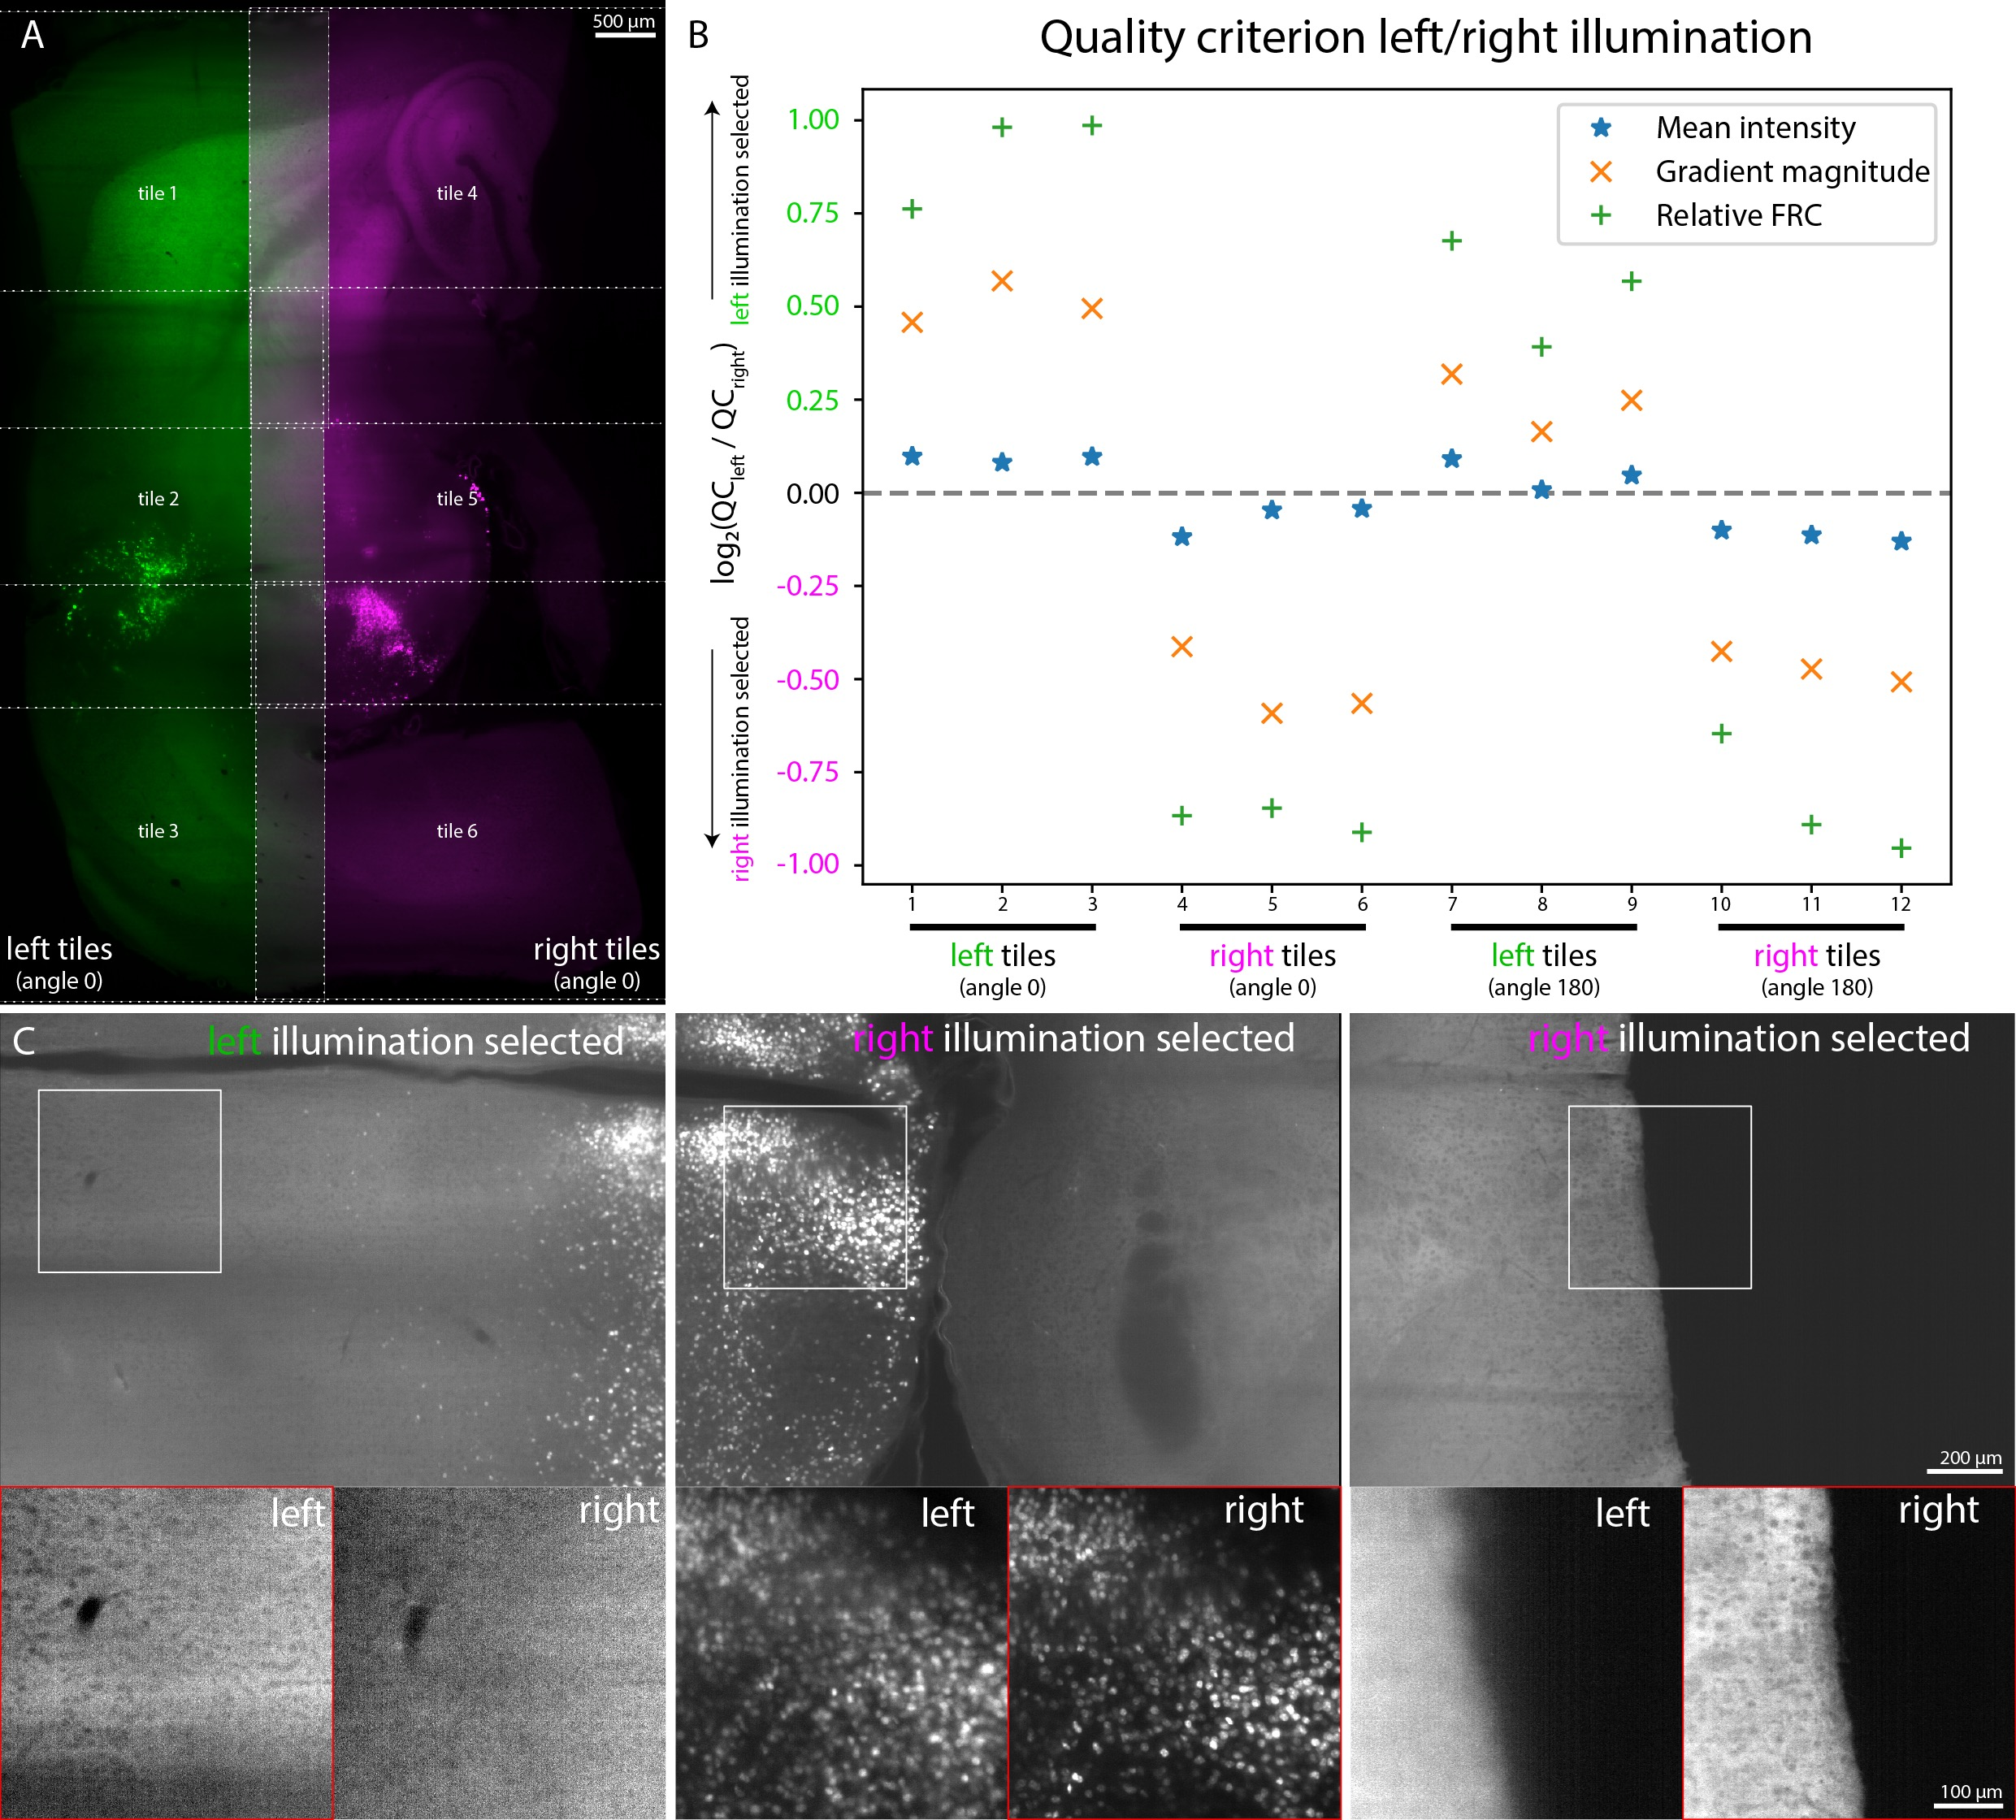
\includegraphics[width=\textwidth]{fig-Illumination-Select.jpg}
\vspace{-2.0mm}
\caption{\hspace{-0.5mm} \red{\emph{Automatic illumination selection.} \textbf{(A)} A small 166GB multi-view, dual-illumination, multi-tile dataset specifically acquired for verification purposes, here to quantify the properties of automatic illumination selection. Shown is a slice through the first of two angles, where six tiles and two illumination directions are highlighted. We manually confirmed that the left three tiles need to be assigned to left illumination, and the right three tiles to right illumination. \textbf{(B)} compares the distinction power of the methods \emph{Mean intensity}, \emph{Gradient magnitude}, and \emph{Relative Fourier Ring Correlation} (see \textbf{Online Methods}) by their respective quality scores. All methods correctly predict the assignment, while the \emph{Relative Fourier Ring Correlation} distinguishes the illumination directions best. Note that \emph{Mean intensity} almost produces an error for tile~8 of the second angle (180 degrees)} \textbf{(C)} Another example of best illumination for three consecutive tiles (left to right), selected based on \emph{Mean intensity} for each tile. Close-ups shows the specified region for both illumination directions. \textbf{(A,C)} As part of this publication automatic illumination selection was performed on 4 datasets (see also \textbf{Fig. 1d, 3b, 3d}).
}
\label{fig:sup-fig-illu-select}
\end{figure*}

\pagebreak

\subsection*{\red{SUPPLEMENTARY FIGURE 3: Chromatic aberration correction}}
\vspace{1mm}
\begin{figure*}[h!]
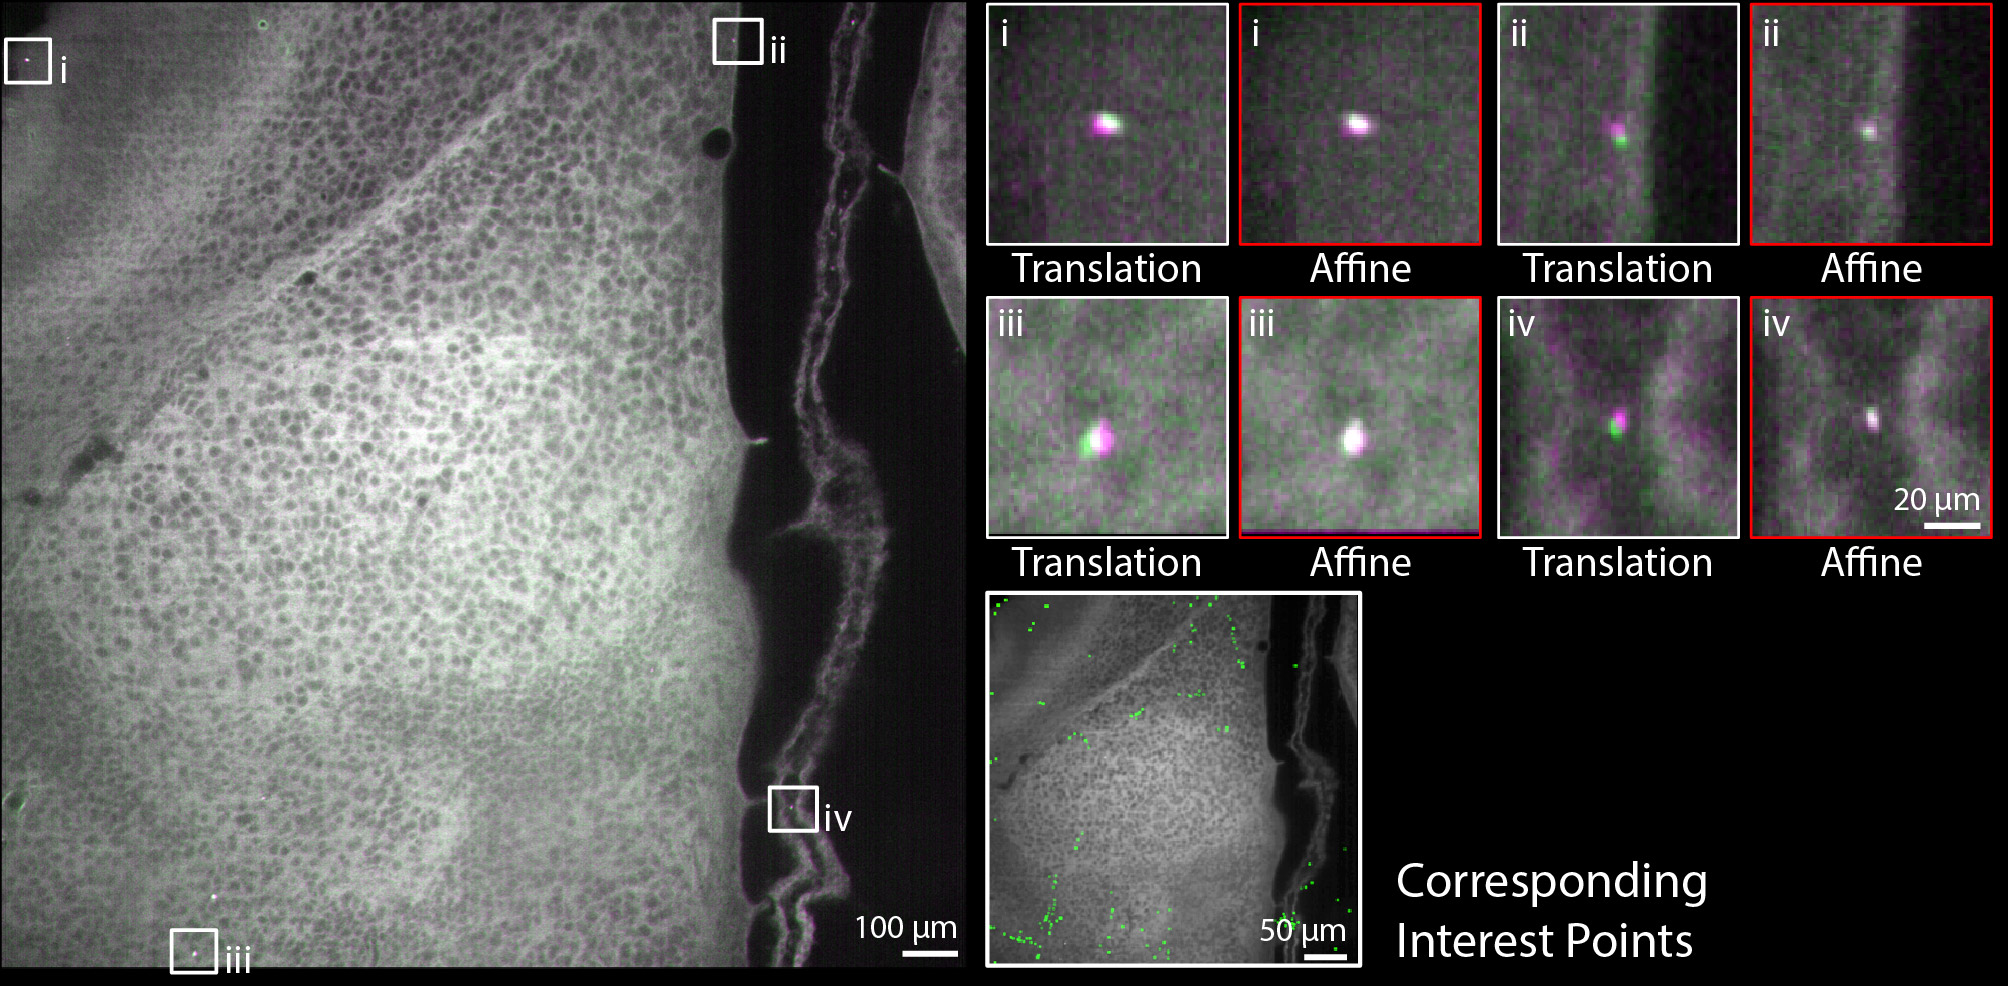
\includegraphics[width=\textwidth]{fig-chr_aberrations.jpg}
\vspace{-2.0mm}
\caption{\hspace{-0.5mm} \red{\emph{Chromatic aberration correction.} If sufficient autofluorescent signal is in common between channels the ICP refinement on an affine model can be used to approximately correct chromatic aberrations are within the range of a few pixels. Here, the 488 and 561 channels are shown in magenta and green, respectively. Zoom-ins (i) -- (iv) illustrate the correction on one example image tile 1920$\times$1920 pixels in size. In the bottom right the interest points (all points of the entire stack are shown for one slice) used for alignment are shown. Please note that for example the point in zoom-in (ii) was not used for alignment. If aberrations are significantly bigger than illustrated in this example or if not enough common autofluorescence between channels exist, images can be preprocessed with dedicated chromatic aberration software before import into BigStitcher (see Limitations section in \textbf{Online Methods}). Chromatic aberration correction was applied to all 26 image tiles of this dataset (\textbf{Suppl. Video 1}) as well as to all cleared samples that were acquired with 2 channels (\textbf{Suppl. Table 1}).
}}
\label{fig:sup-chromatic}
\end{figure*}

\pagebreak

\subsection*{\red{SUPPLEMENTARY FIGURE 4: Spherical aberration correction}}
\vspace{-2mm}
\begin{figure*}[h!]
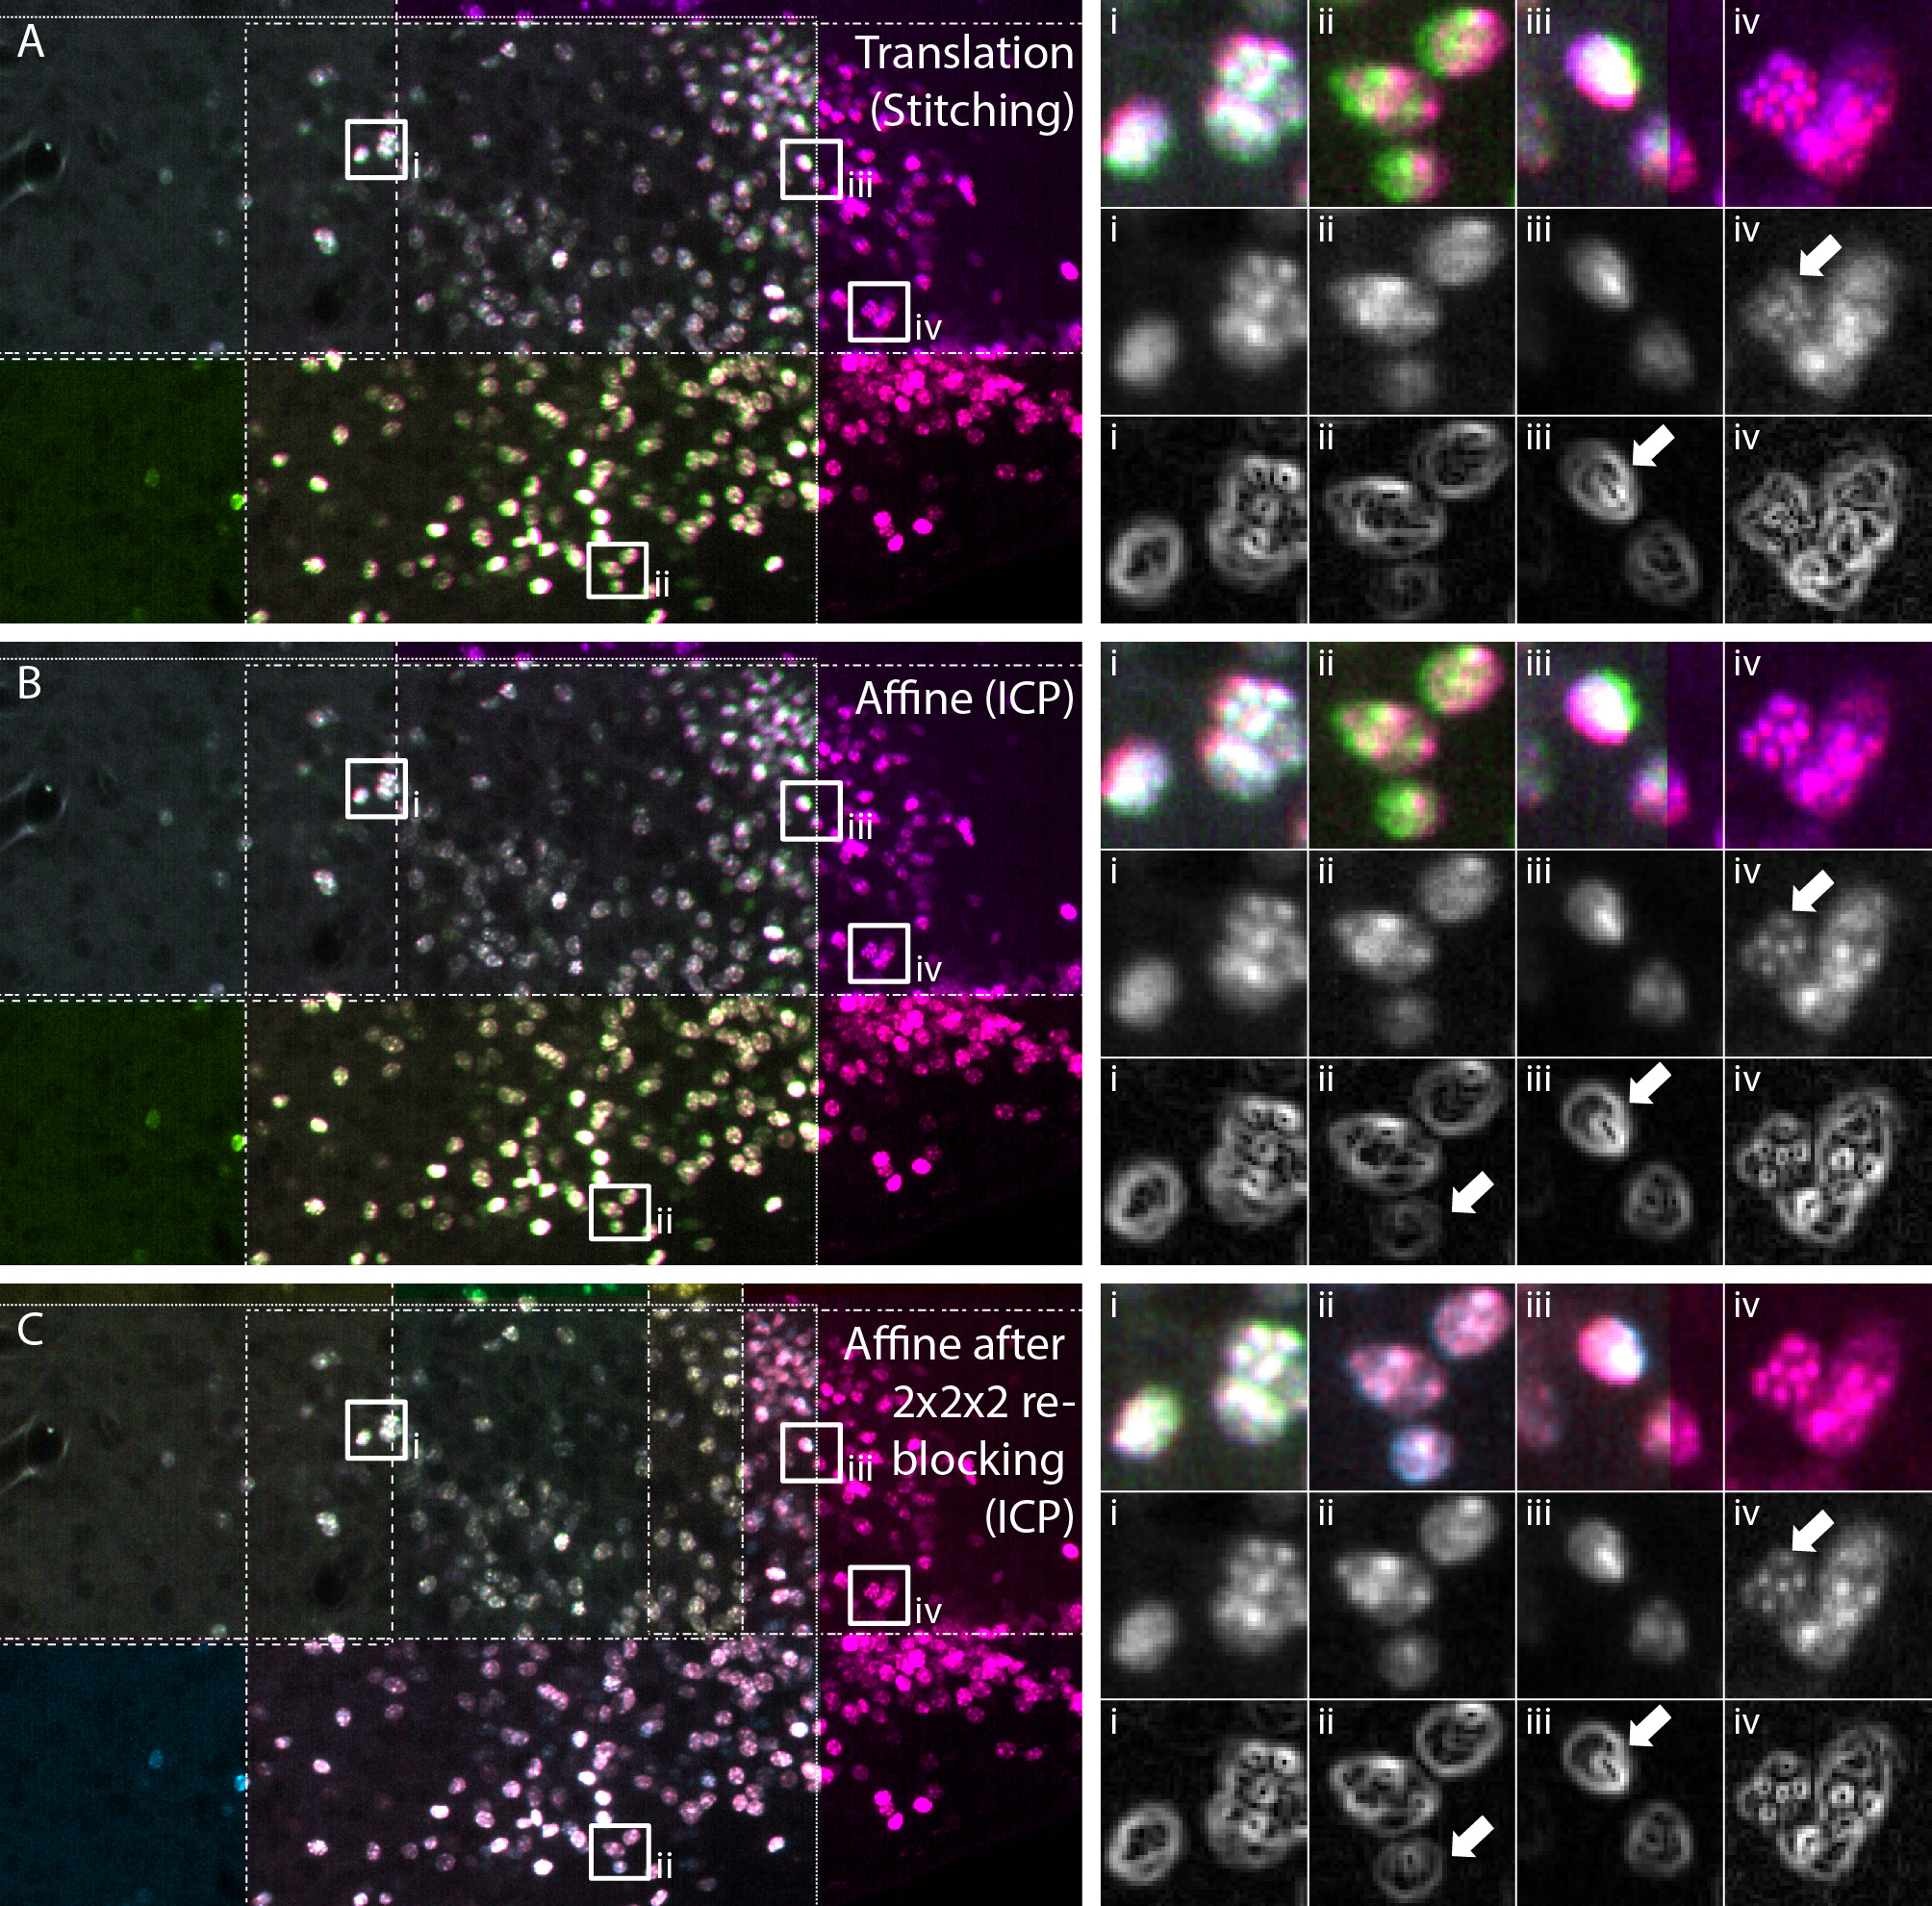
\includegraphics[width=\textwidth]{fig-sph_aberrations.jpg}
\vspace{-3mm}
\caption{\hspace{-0.5mm} \red{\emph{Spherical aberration correction.} \textbf{(A-C)} show the same area a cleared adult mouse hypothalamus expressing H2B-GFP in all bsx neurons where the corners of 4 image tiles of the same wavelength overlap. Zoom-ins (i)--(iv) show the alignment quality by overlaying different colors (1st row), after image fusing using blending (2nd row), and the sobel-filtering of the blending fusion (3rd row). \textbf{(A)}~shows results for stitching, \textbf{(B)} when using affine refinement, and \textbf{(C)} when using affine refinement on re-blocked images. Note that affine, and split-affine improve the alignment quality. Blending-fusion can reduce artifacts as it reduces the contribution of pixels close to image borders. Arrows outline cases where artifacts persist after blending-fusion. E.g., the artifact visible in the fusion in (iii) stems from misalignments of the pink and red tile, since the green tile is almost invisible after fusion. \textbf{(A-C)} Spherical aberration correction using affine transformations achieving similar results was applied to all 26 tiles of the dataset, as well as the datasets shown in (\textbf{Fig. 1n, 3b-d}). 
}}
\label{fig:sup-spherical}
\end{figure*}

\pagebreak


\subsection*{SUPPLEMENTARY FIGURE 5: Manual alignment}
\vspace{1mm}
\begin{figure*}[h!]
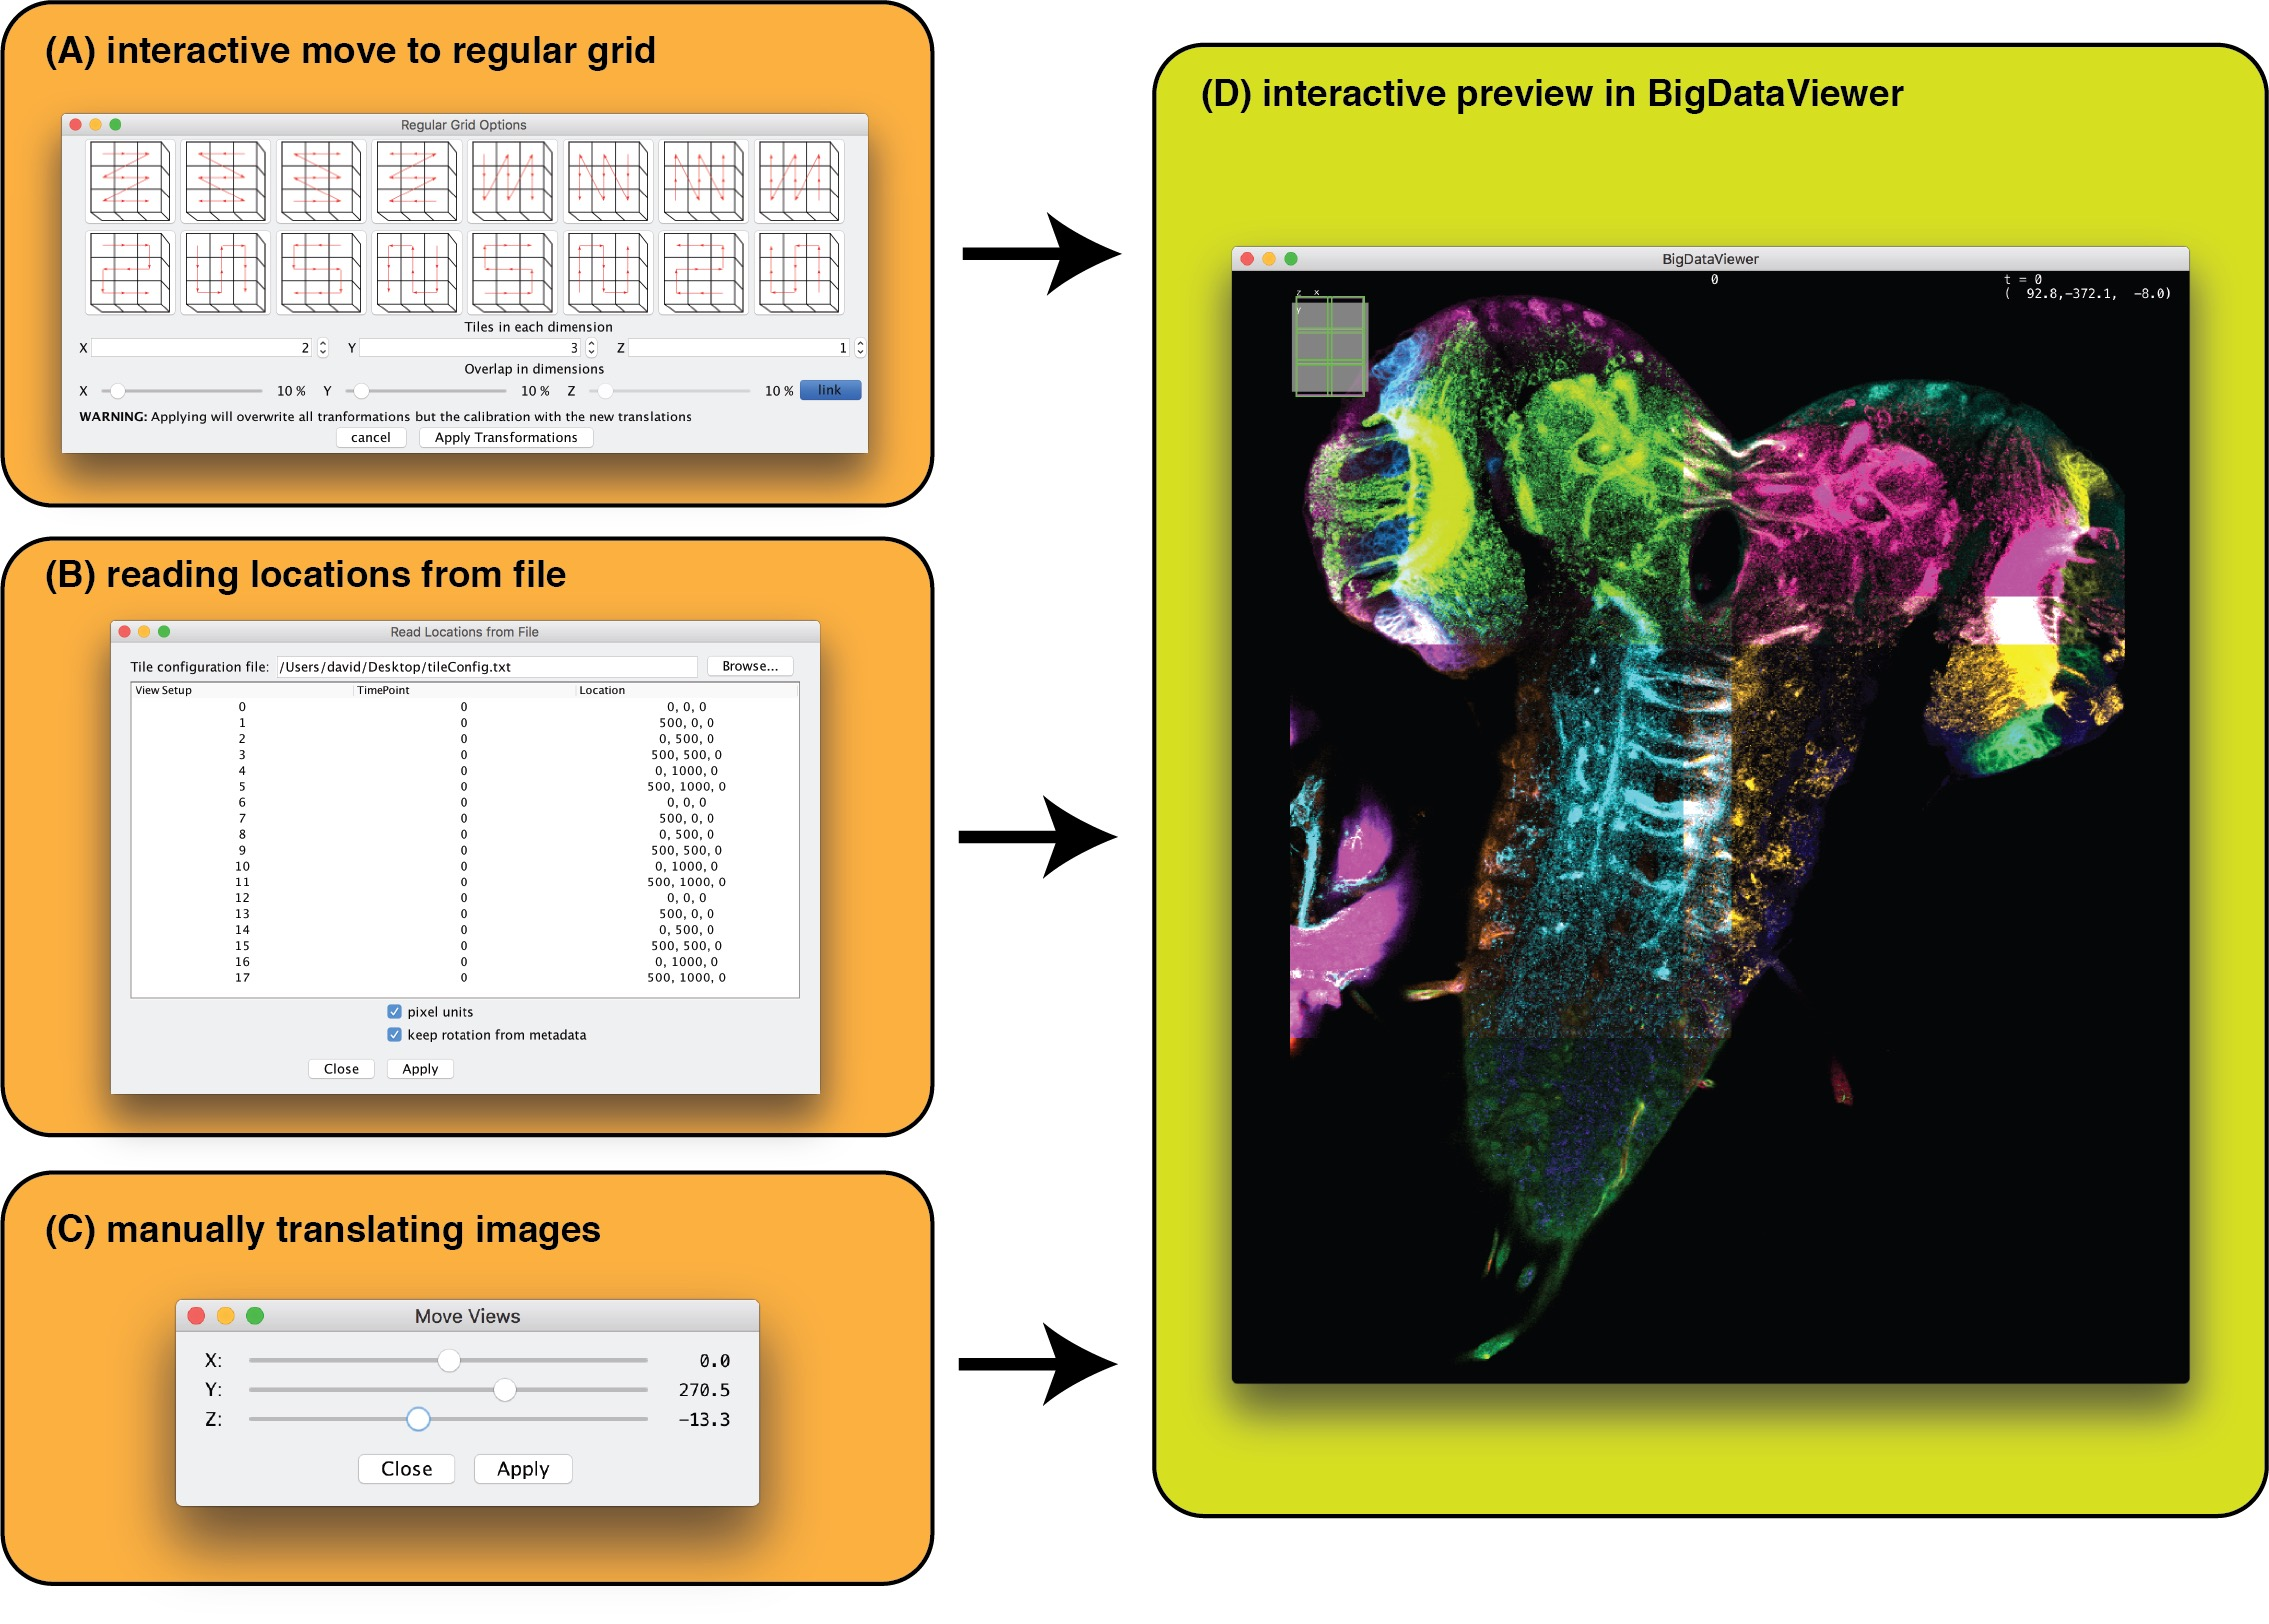
\includegraphics[width=\textwidth]{manual-view-arrangement.jpg}
\vspace{-2.0mm}
\caption{\hspace{-0.5mm} \emph{Interactive manual alignment of tiled images.} The BigStitcher GUI offers various ways of manually (pre-)aligning tiled images after import. \textbf{(A)} images can be moved to a regular grid with a given tile order and overlap. \textbf{(B)} image locations can also be read from a simple \emph{tile configuration} text file. \textbf{(C)} selected image(s) can be moved along axes via sliders. \textbf{(D)} all changes will be displayed in the BigDataViewer window immediately \textbf{(D)} for quick verification. 
}
\label{fig:sup-fig-manual-align1}
\end{figure*}

\pagebreak

\subsection*{SUPPLEMENTARY FIGURE 6: Flat-field correction}
\vspace{1mm}
\begin{figure*}[h!]
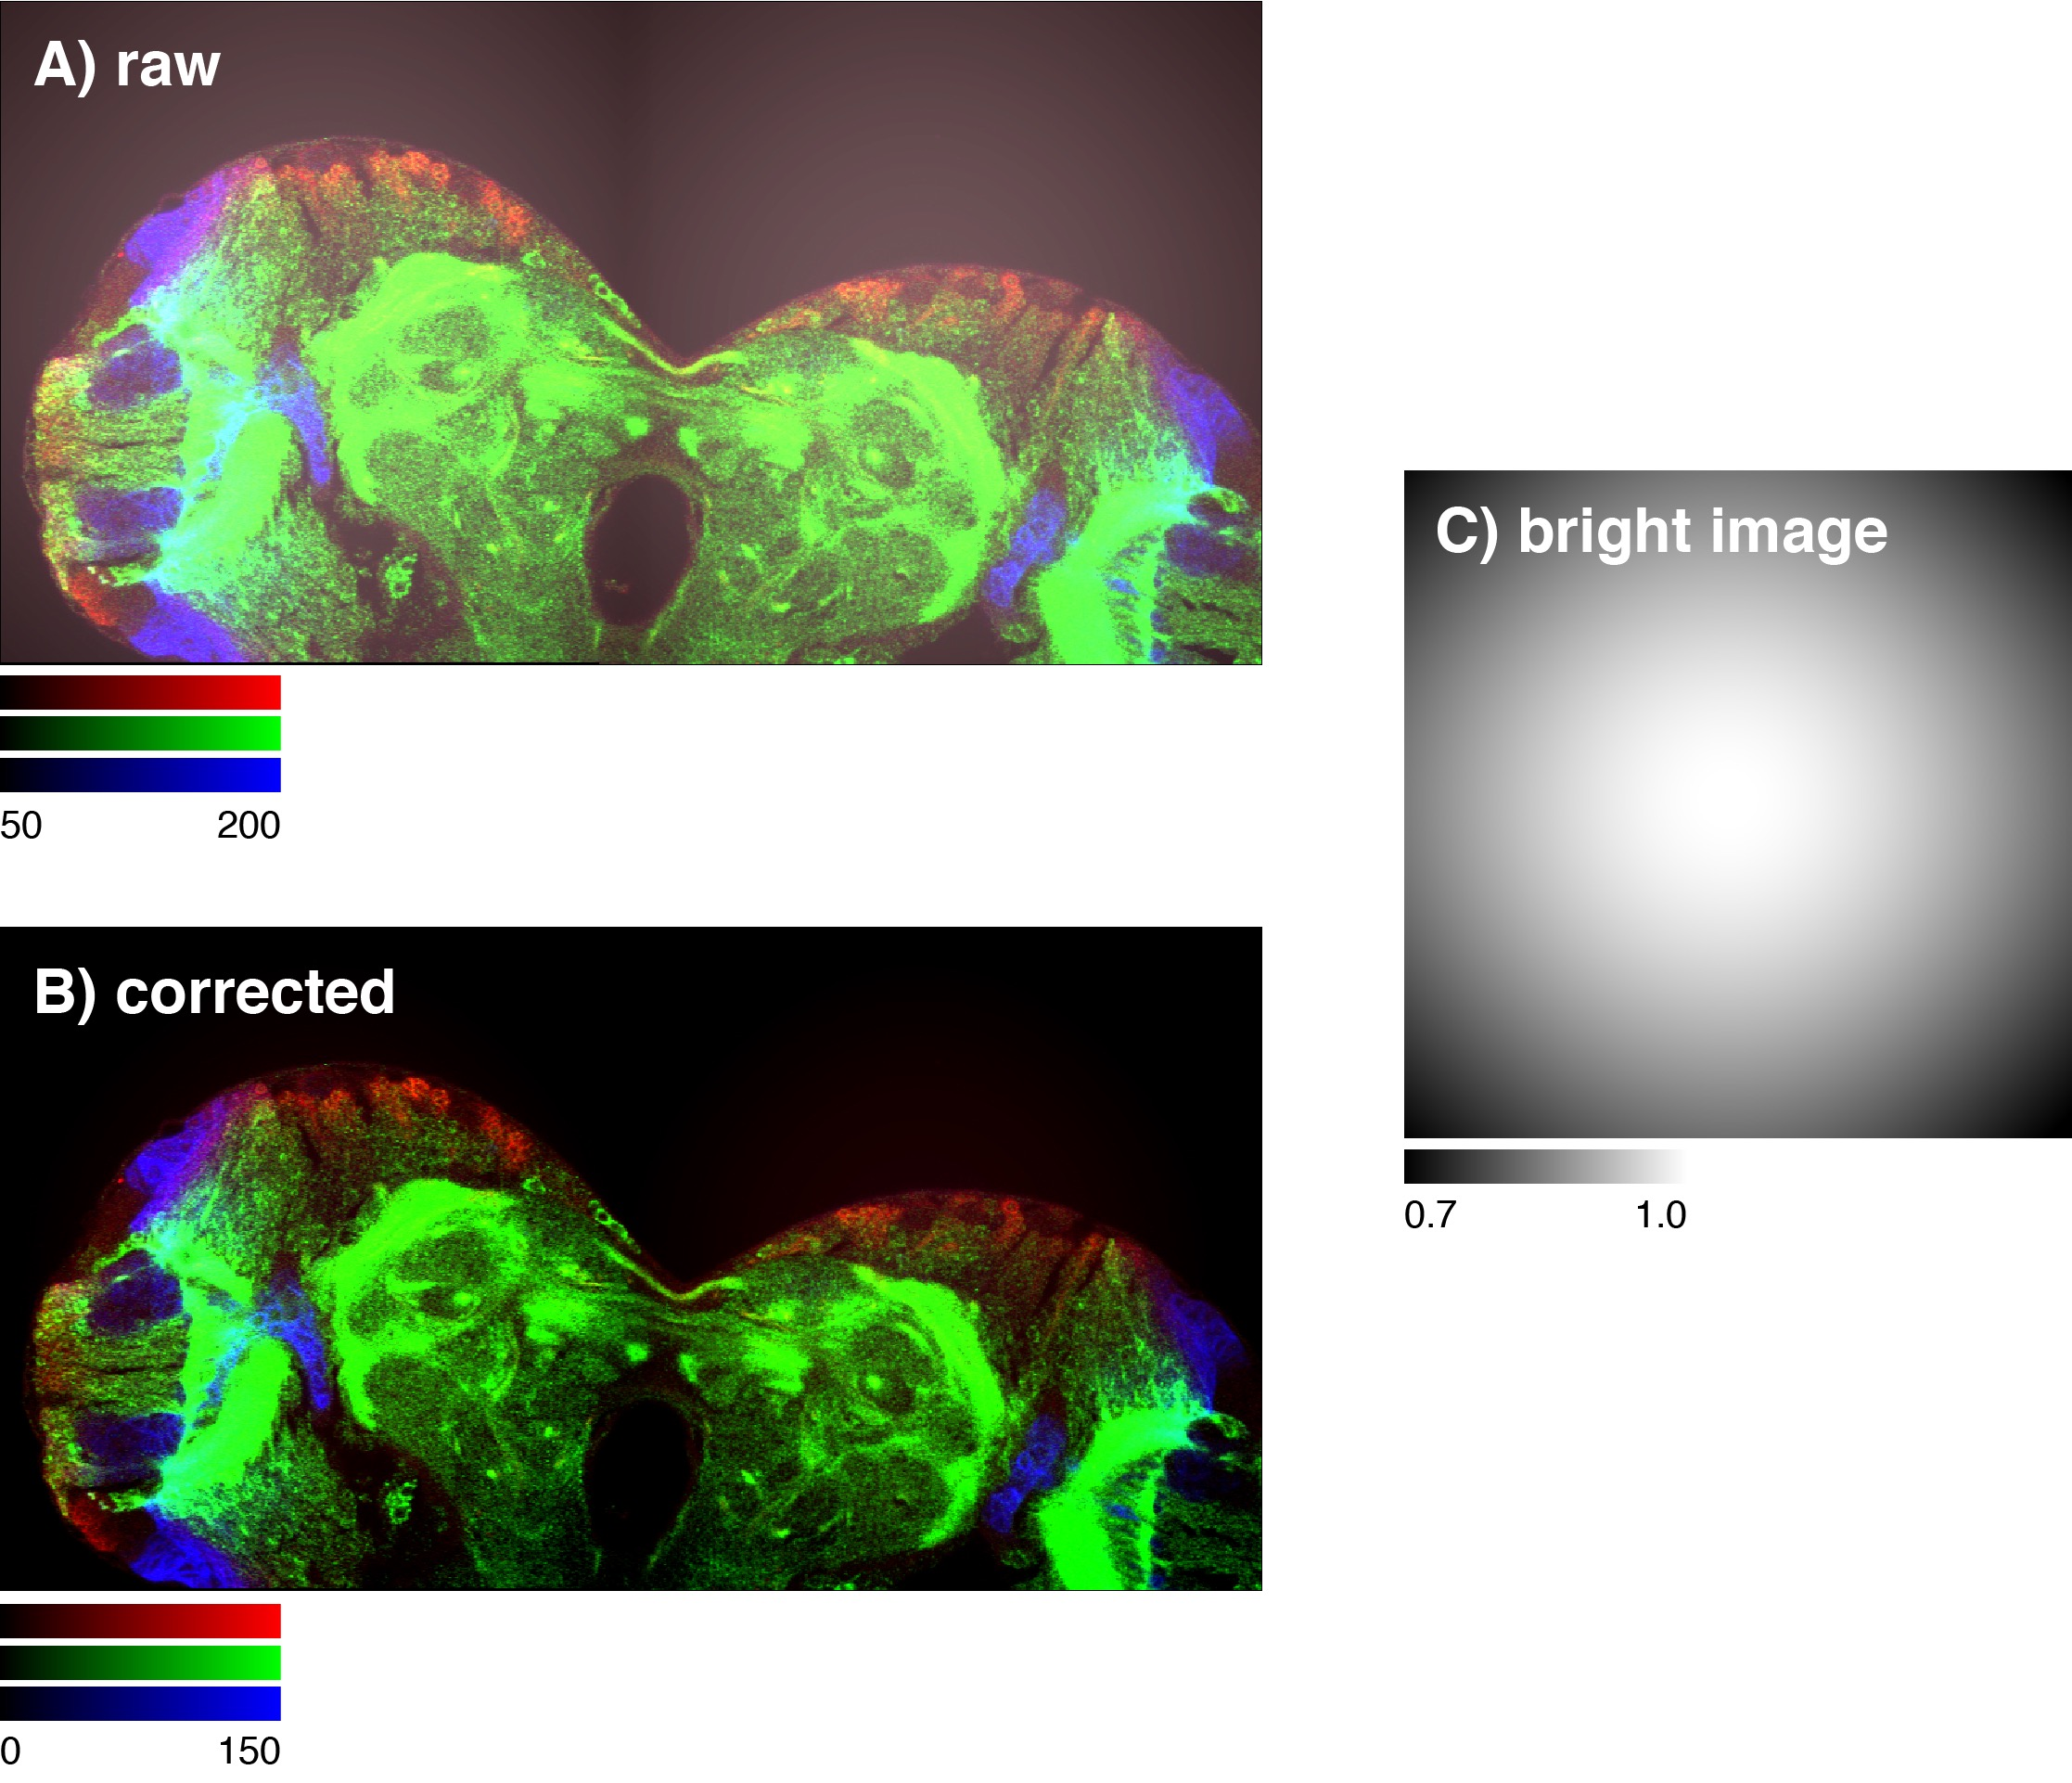
\includegraphics[width=\textwidth]{fig-flatfield.jpg}
\vspace{-2.0mm}
\caption{\hspace{-0.5mm} \emph{On-the-fly flat-field correction.} The BigStitcher offers correction for camera offsets, fixed pattern noise or uneven illumination. \textbf{(A)}  Simulation of the effects of a constant background offset and Gaussian illumination/detection efficiency \textbf{(C)} on tiled images. By subtracting the \emph{dark image} and modulating with the inverse relative intensity of the \emph{bright image}, such artifacts can be corrected easily \textbf{(B)}. The correction is calculated virtually, with optional caching, to allow for immediate inspection of the results. \textbf{(A-C)} Flatfield correction as illustrated in this figure is a feature supported by BigStitcher, but has not been applied to any of the datasets shown in this publication.
}
\label{fig:sup-fig-flatfield}
\end{figure*}

\pagebreak

\subsection*{\red{SUPPLEMENTARY FIGURE 7: Automatic quantification of image quality}}
\vspace{1mm}
\begin{figure*}[h!]
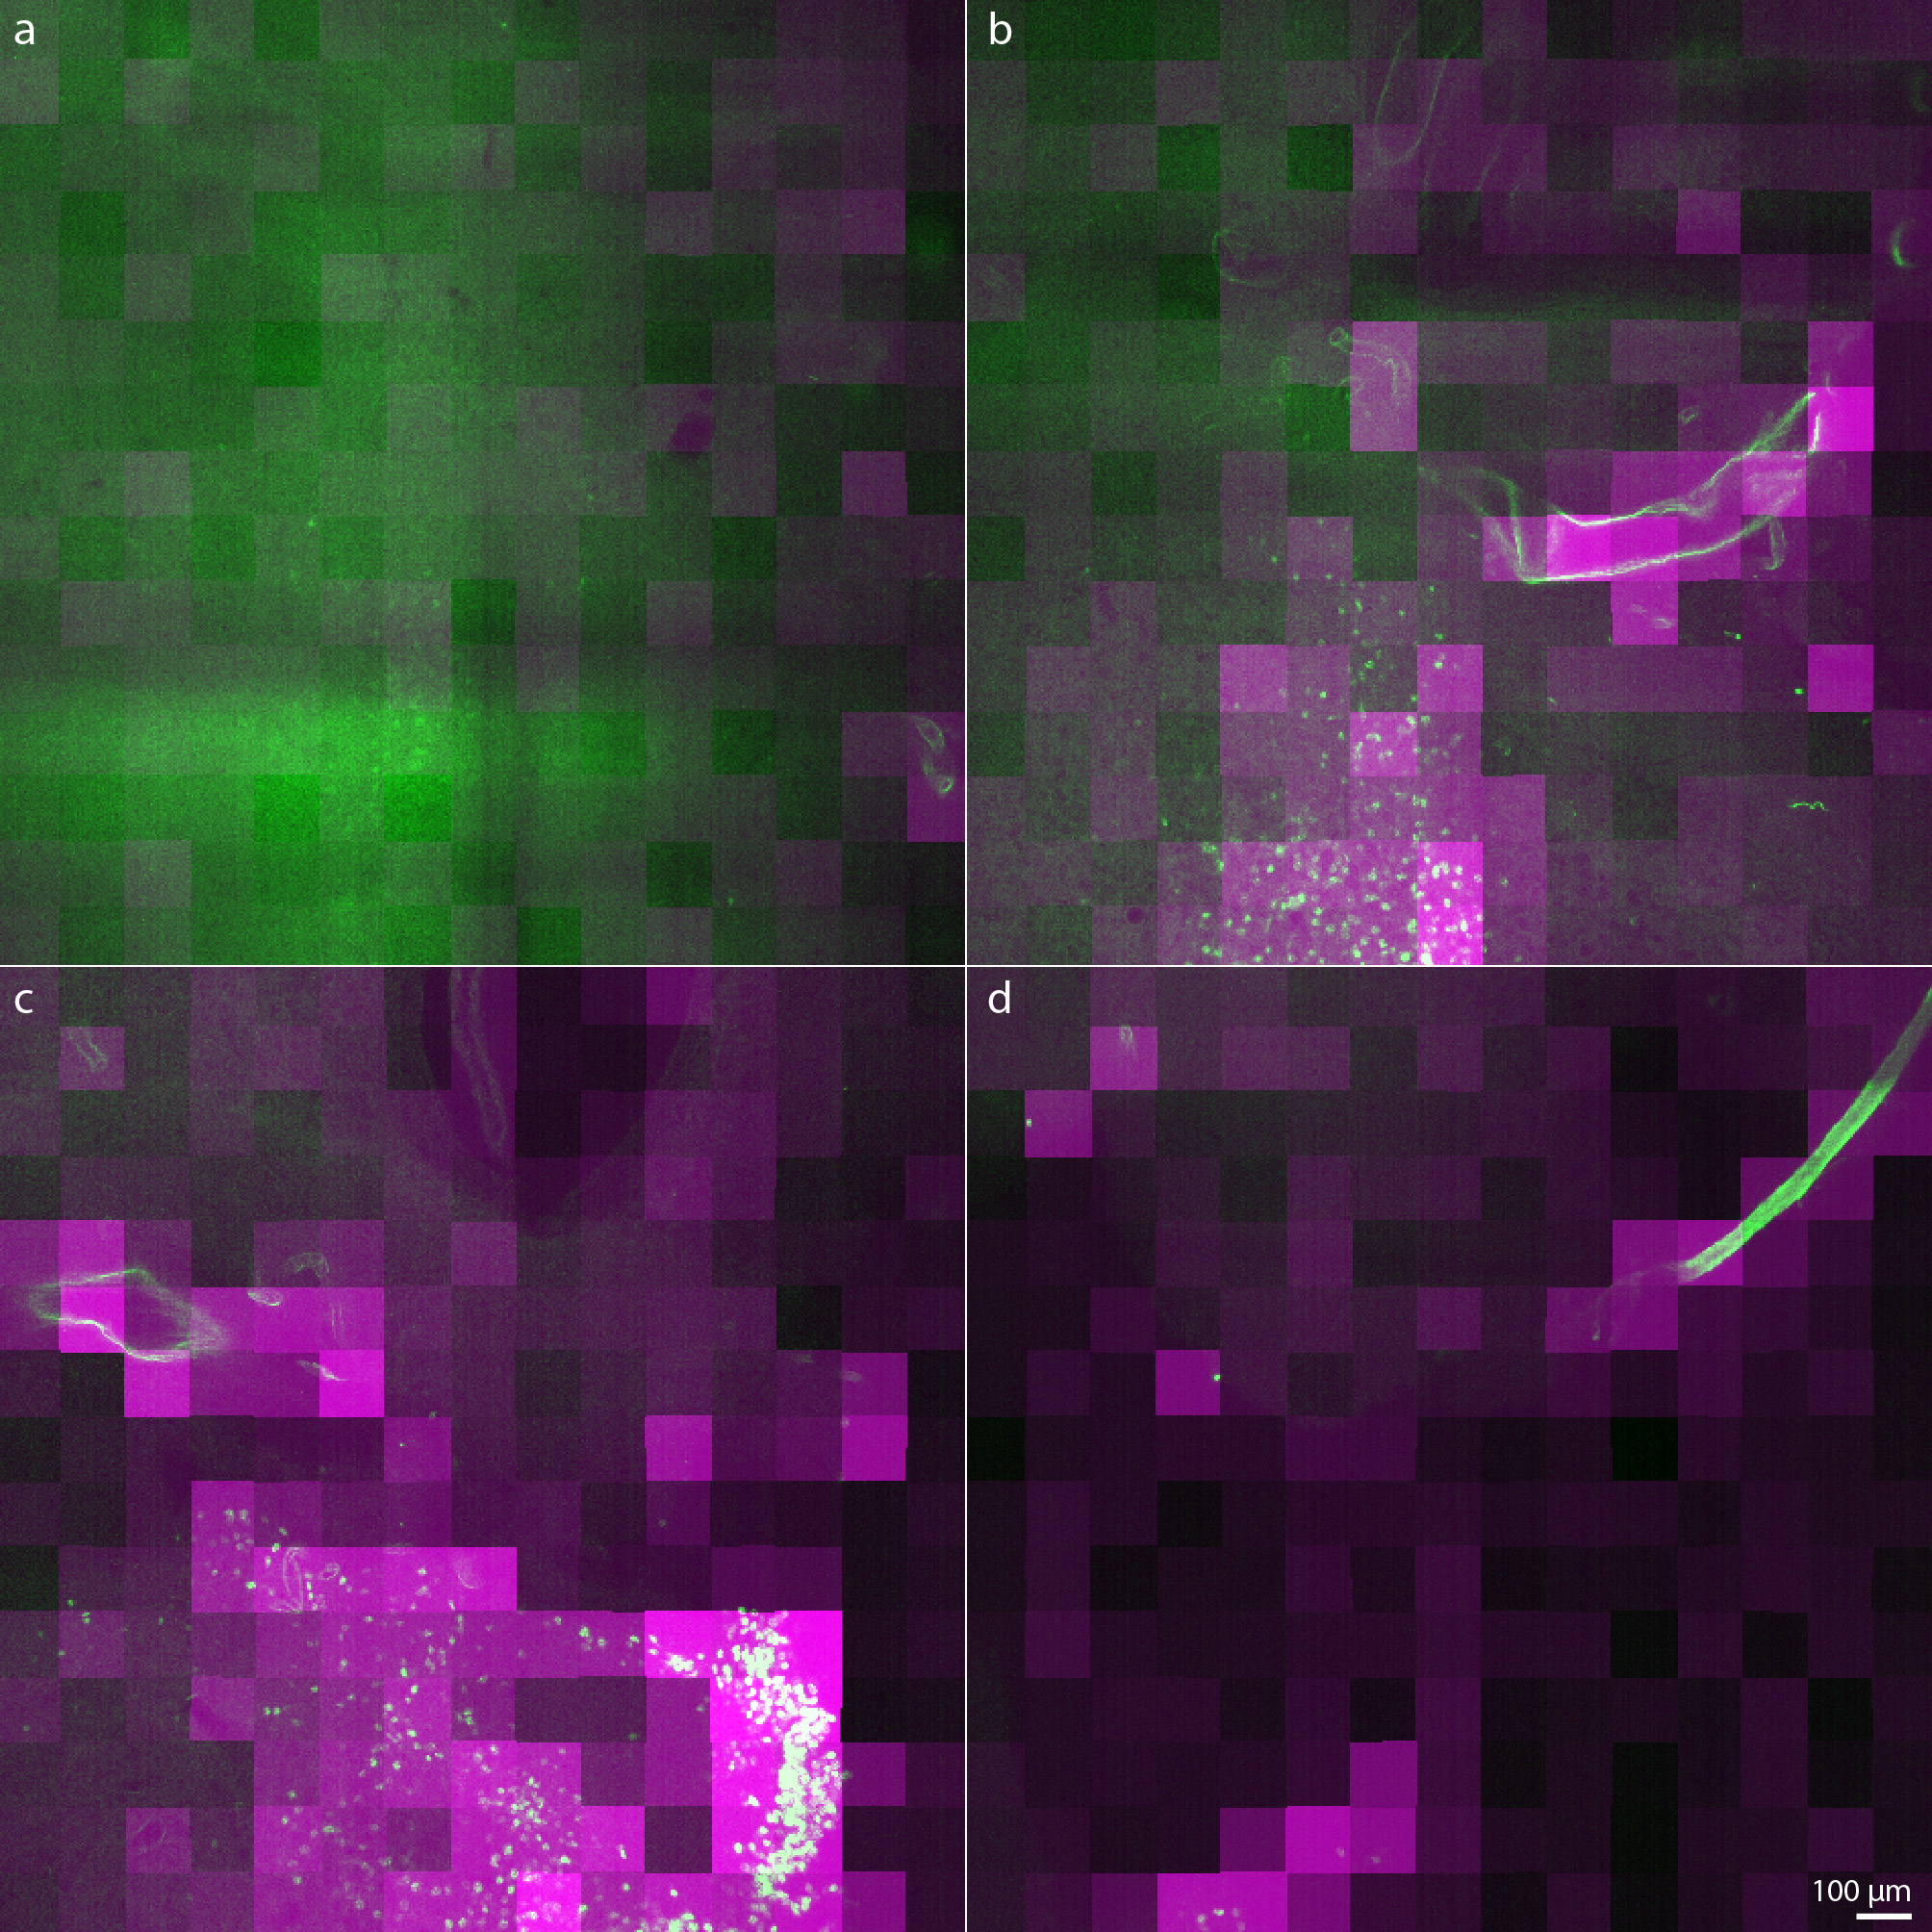
\includegraphics[width=\textwidth]{rFRC.jpg}
\vspace{-2.0mm}
\caption{\hspace{-0.5mm} \red{\emph{Automatic Quantification of Image Quality.} \textbf{(a-d)} Four different z-planes from a volume that overlays the results of the relative Fourier Ring Correlation (rFRC, see \textbf{Online Methods}) computed in 128$\times$128 blocks using a spacing of 10 pixels (magenta) and cleared image data (same as \textbf{Suppl. Fig. \ref{fig:sup-fig-rf}}). The rFRC robustly detects areas with high image quality. Note that (a) is deepest inside the tissue and (d) is at the surface of the sample. See \textbf{Suppl. Video 8} for an animation of the entire stack. The rFRC was successfully applied to all cleared datasets in this publication (\textbf{Suppl. Table 1}), results are also shown in \textbf{Suppl. Fig. \ref{fig:sup-fig-rf}, \ref{fig:sup-rfrc-brain}} and \textbf{Suppl. Video 8,9}.
}}
\label{fig:sup-rFRC}
\end{figure*}

\pagebreak

\subsection*{\red{SUPPLEMENTARY FIGURE 8: Quality estimation in whole-brain mouse acquisition}}
\vspace{1mm}
\begin{figure*}[h!]
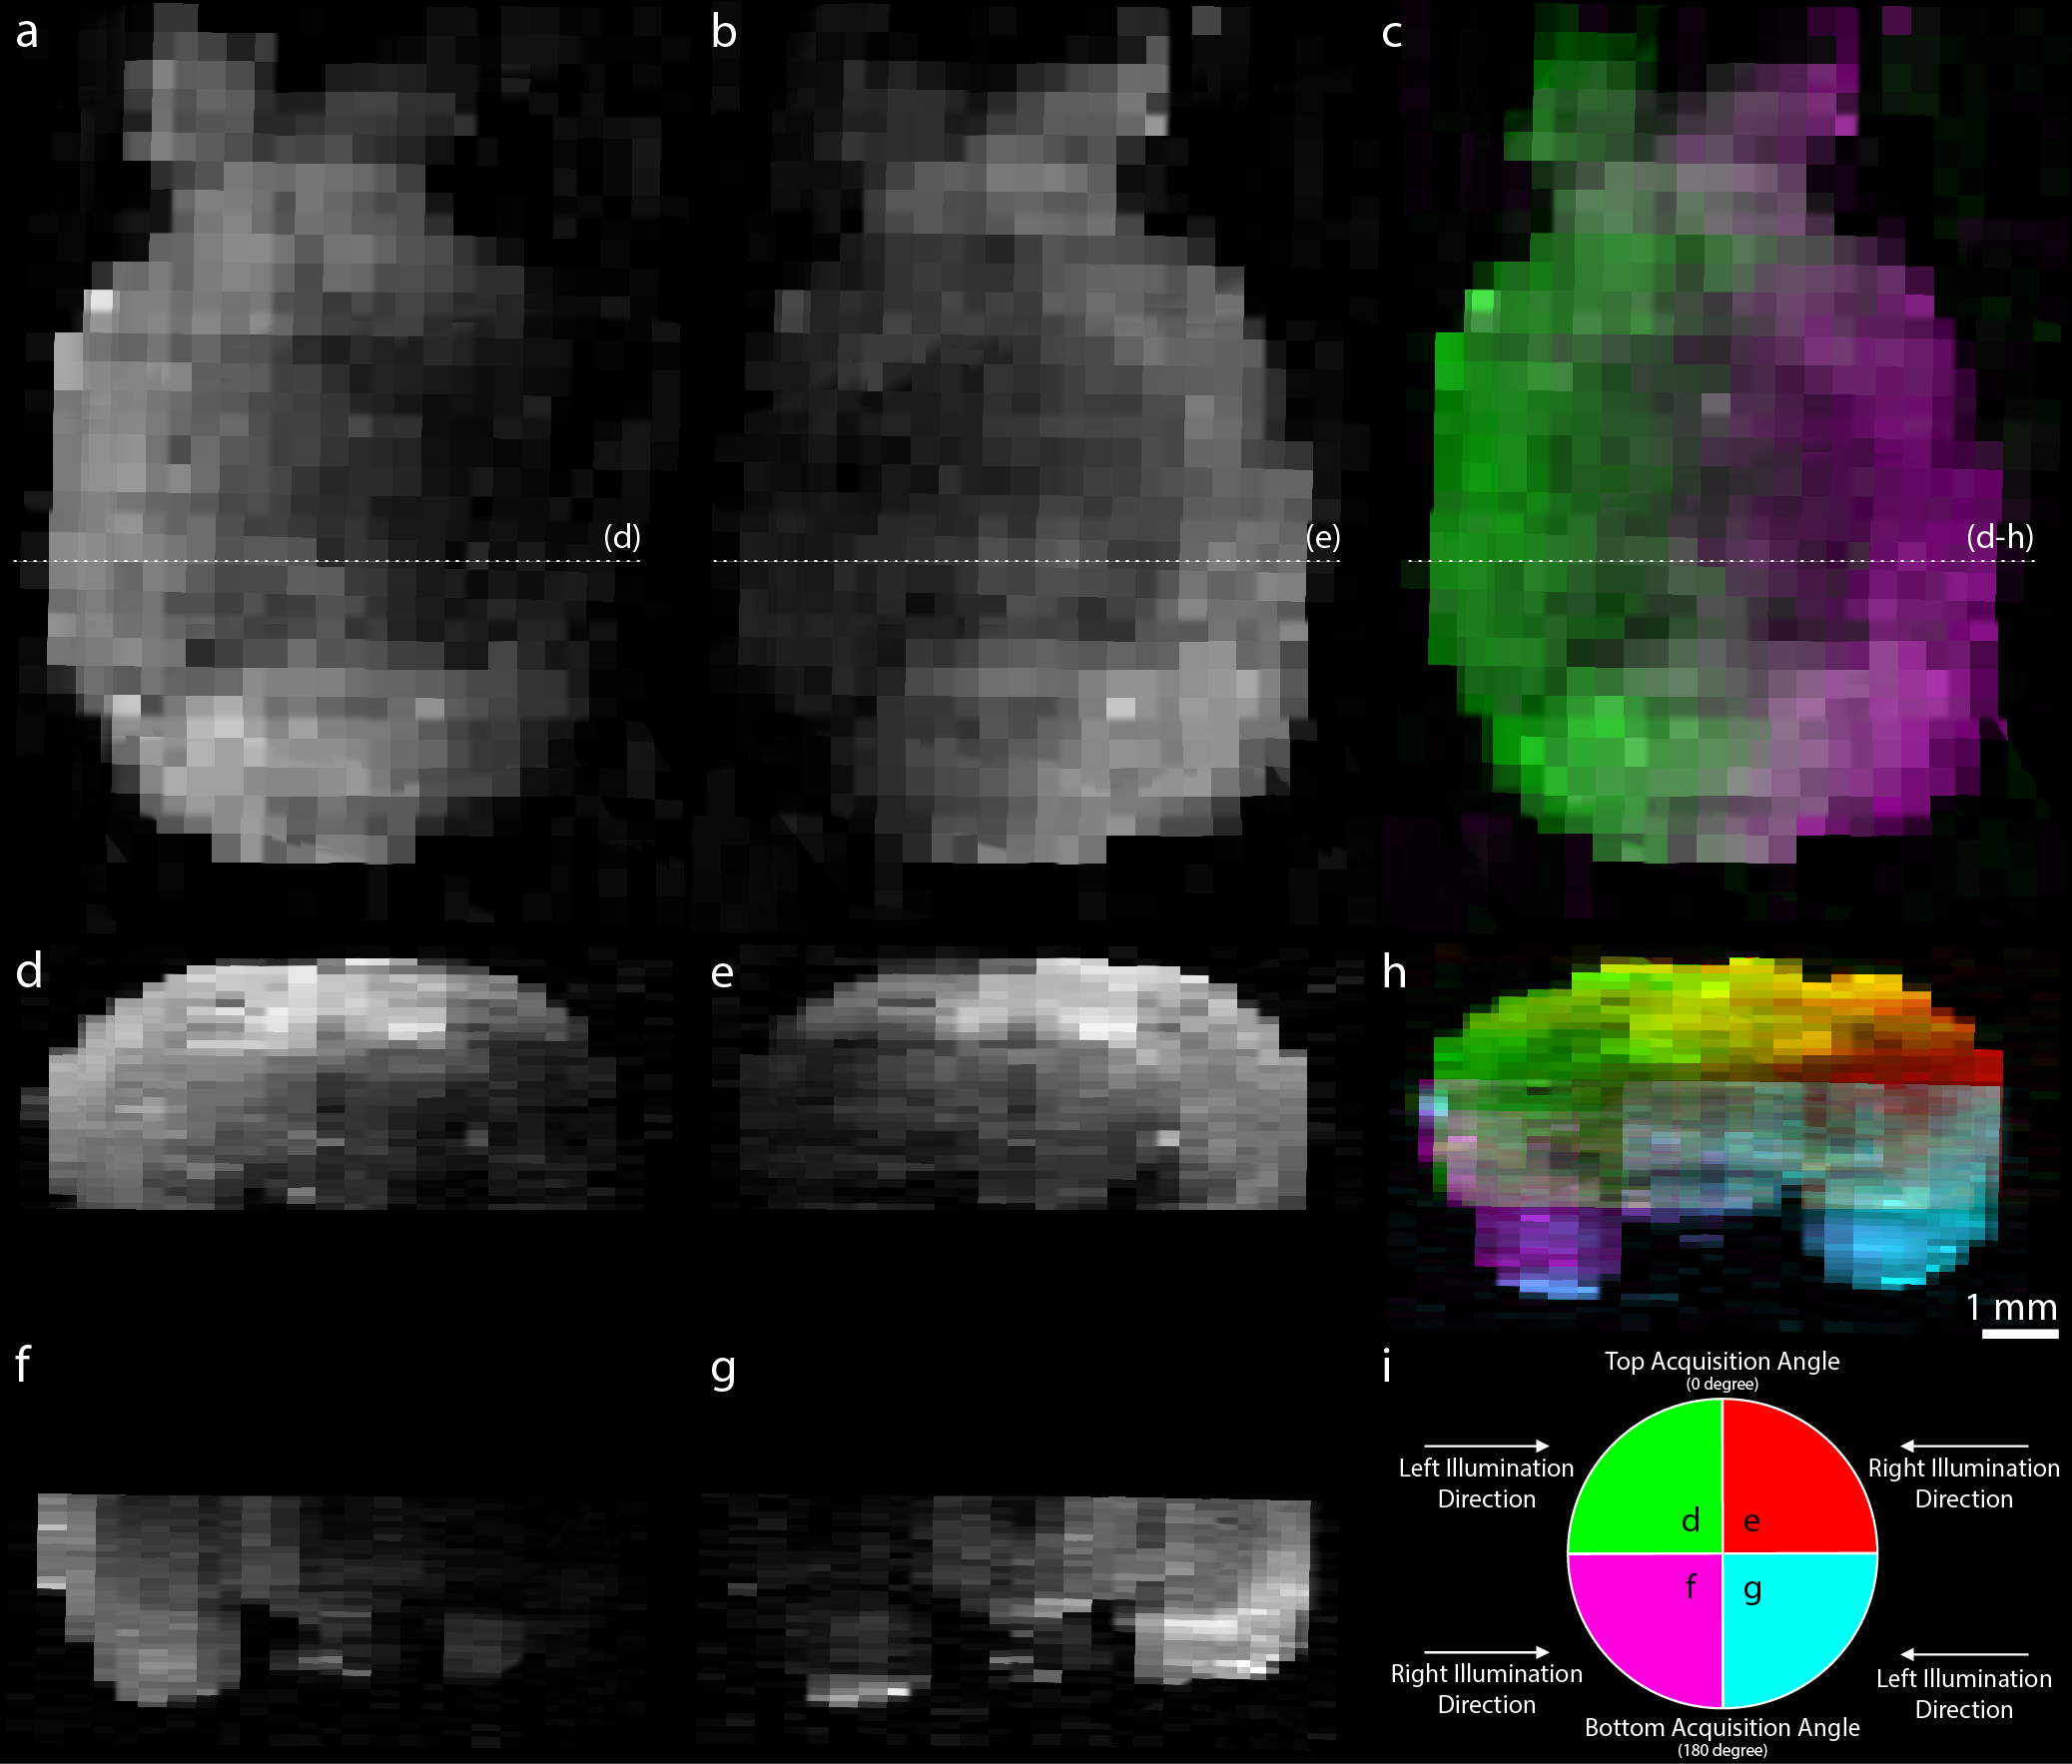
\includegraphics[width=\textwidth]{rFRC_brain.png}
\vspace{-2.0mm}
\caption{\hspace{-0.5mm} \red{\emph{Quality Estimation in Whole-Brain Mouse Acquisition.} Application of our relative Fourier Ring Correlation (rFRC, see \textbf{Online Methods}) to the reconstruction of an entire adult mouse brain. The rFRC was computed in 512$\times$512 blocks using a spacing of 256 pixels and transformed and rendered as the reconstructed volume (see Fig. 3d). \textbf{(a,b,c)} single slice through rFRC volume based on image data acquired with left illumination (a), right illumination (b), and both overlaid (c), dotted lines outline the orthogonal shown views in (d-h). \textbf{(d-h)} orthogonal views to (a-c) highlighting the contribution in image quality from different illumination directions and acquisition angles. \textbf{(i)} illustration of the color scheme used in (h) and the type of data displayed in (d-g). See \textbf{Suppl. Video 9} for an animation of the entire stack. The rFRC was successfully applied to all cleared datasets in this publication (\textbf{Suppl. Table 1}), results are also shown in \textbf{Suppl. Fig. \ref{fig:sup-fig-rf}, \ref{fig:sup-rFRC}} and \textbf{Suppl. Video 8,9}.
}}
\label{fig:sup-rfrc-brain}
\end{figure*}

\pagebreak

\subsection*{SUPPLEMENTARY FIGURE 9: Affine refinement via ICP}
\vspace{-3mm}
\begin{figure*}[h!]
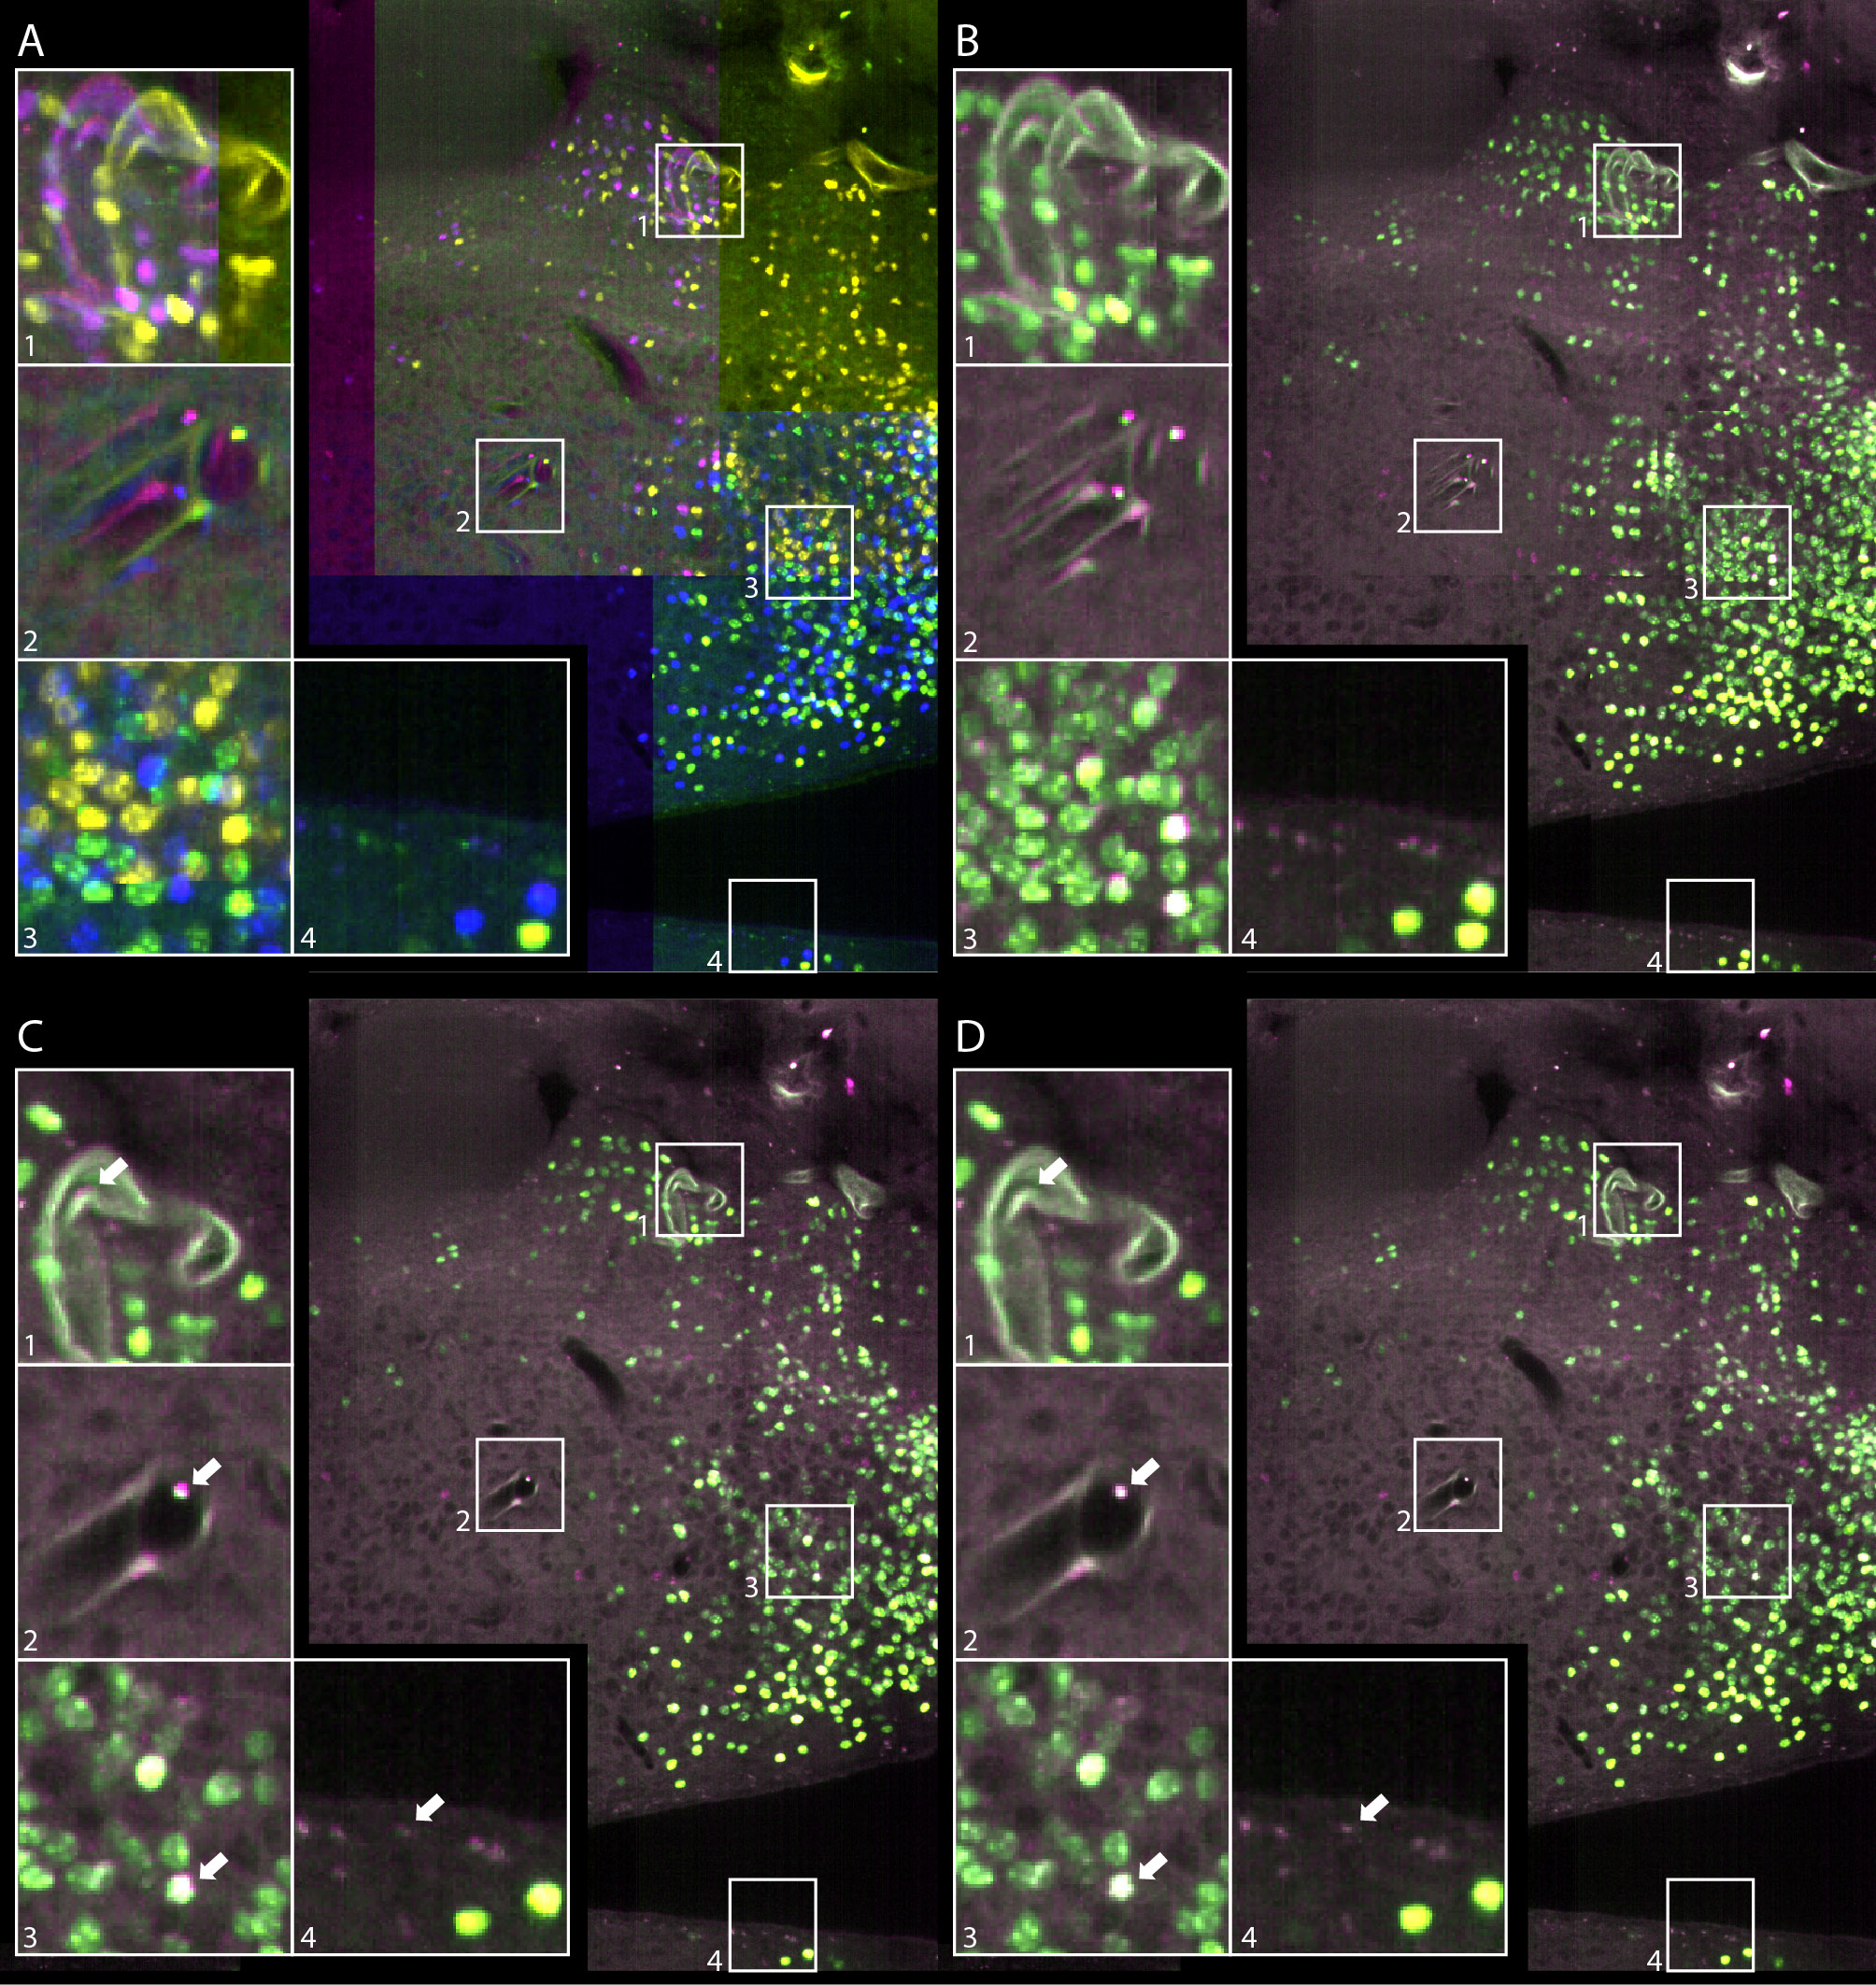
\includegraphics[width=\textwidth]{fig-stitching_icp.jpg}
\vspace{-3.0mm}
\caption{\hspace{-0.5mm} \emph{Illustration of different steps for multi-tile alignment} \textbf{(A)} Four randomly colored, overlapping image tiles show the typical error when using microscope metadata only. \textbf{(B)} Shows the same image tiles as (A), but without random color coding. \textbf{(C)} Quality of the registration after applying the phase-correlation based stitching with downsampling 4 and two-round global optimization. \textbf{(D)} \red{Result after applying the automatic ICP refinement for tile alignment, spherical and chromatic aberration correction. \textbf{(A-D)} Insets highlight specific areas to better appreciate quality differences. \textbf{(A-D)} ICP-refinement using affine transformations achieving similar results was applied to all 26 tiles of the dataset, as well as the datasets shown in (\textbf{Fig. 1n, 3b-d}). 
}}
\label{fig:sup-fig-icp}
\end{figure*}

\pagebreak


\subsection*{SUPPLEMENTARY FIGURE 10: Global optimization}
\vspace{-3mm}
\begin{figure*}[h!]
\centerline{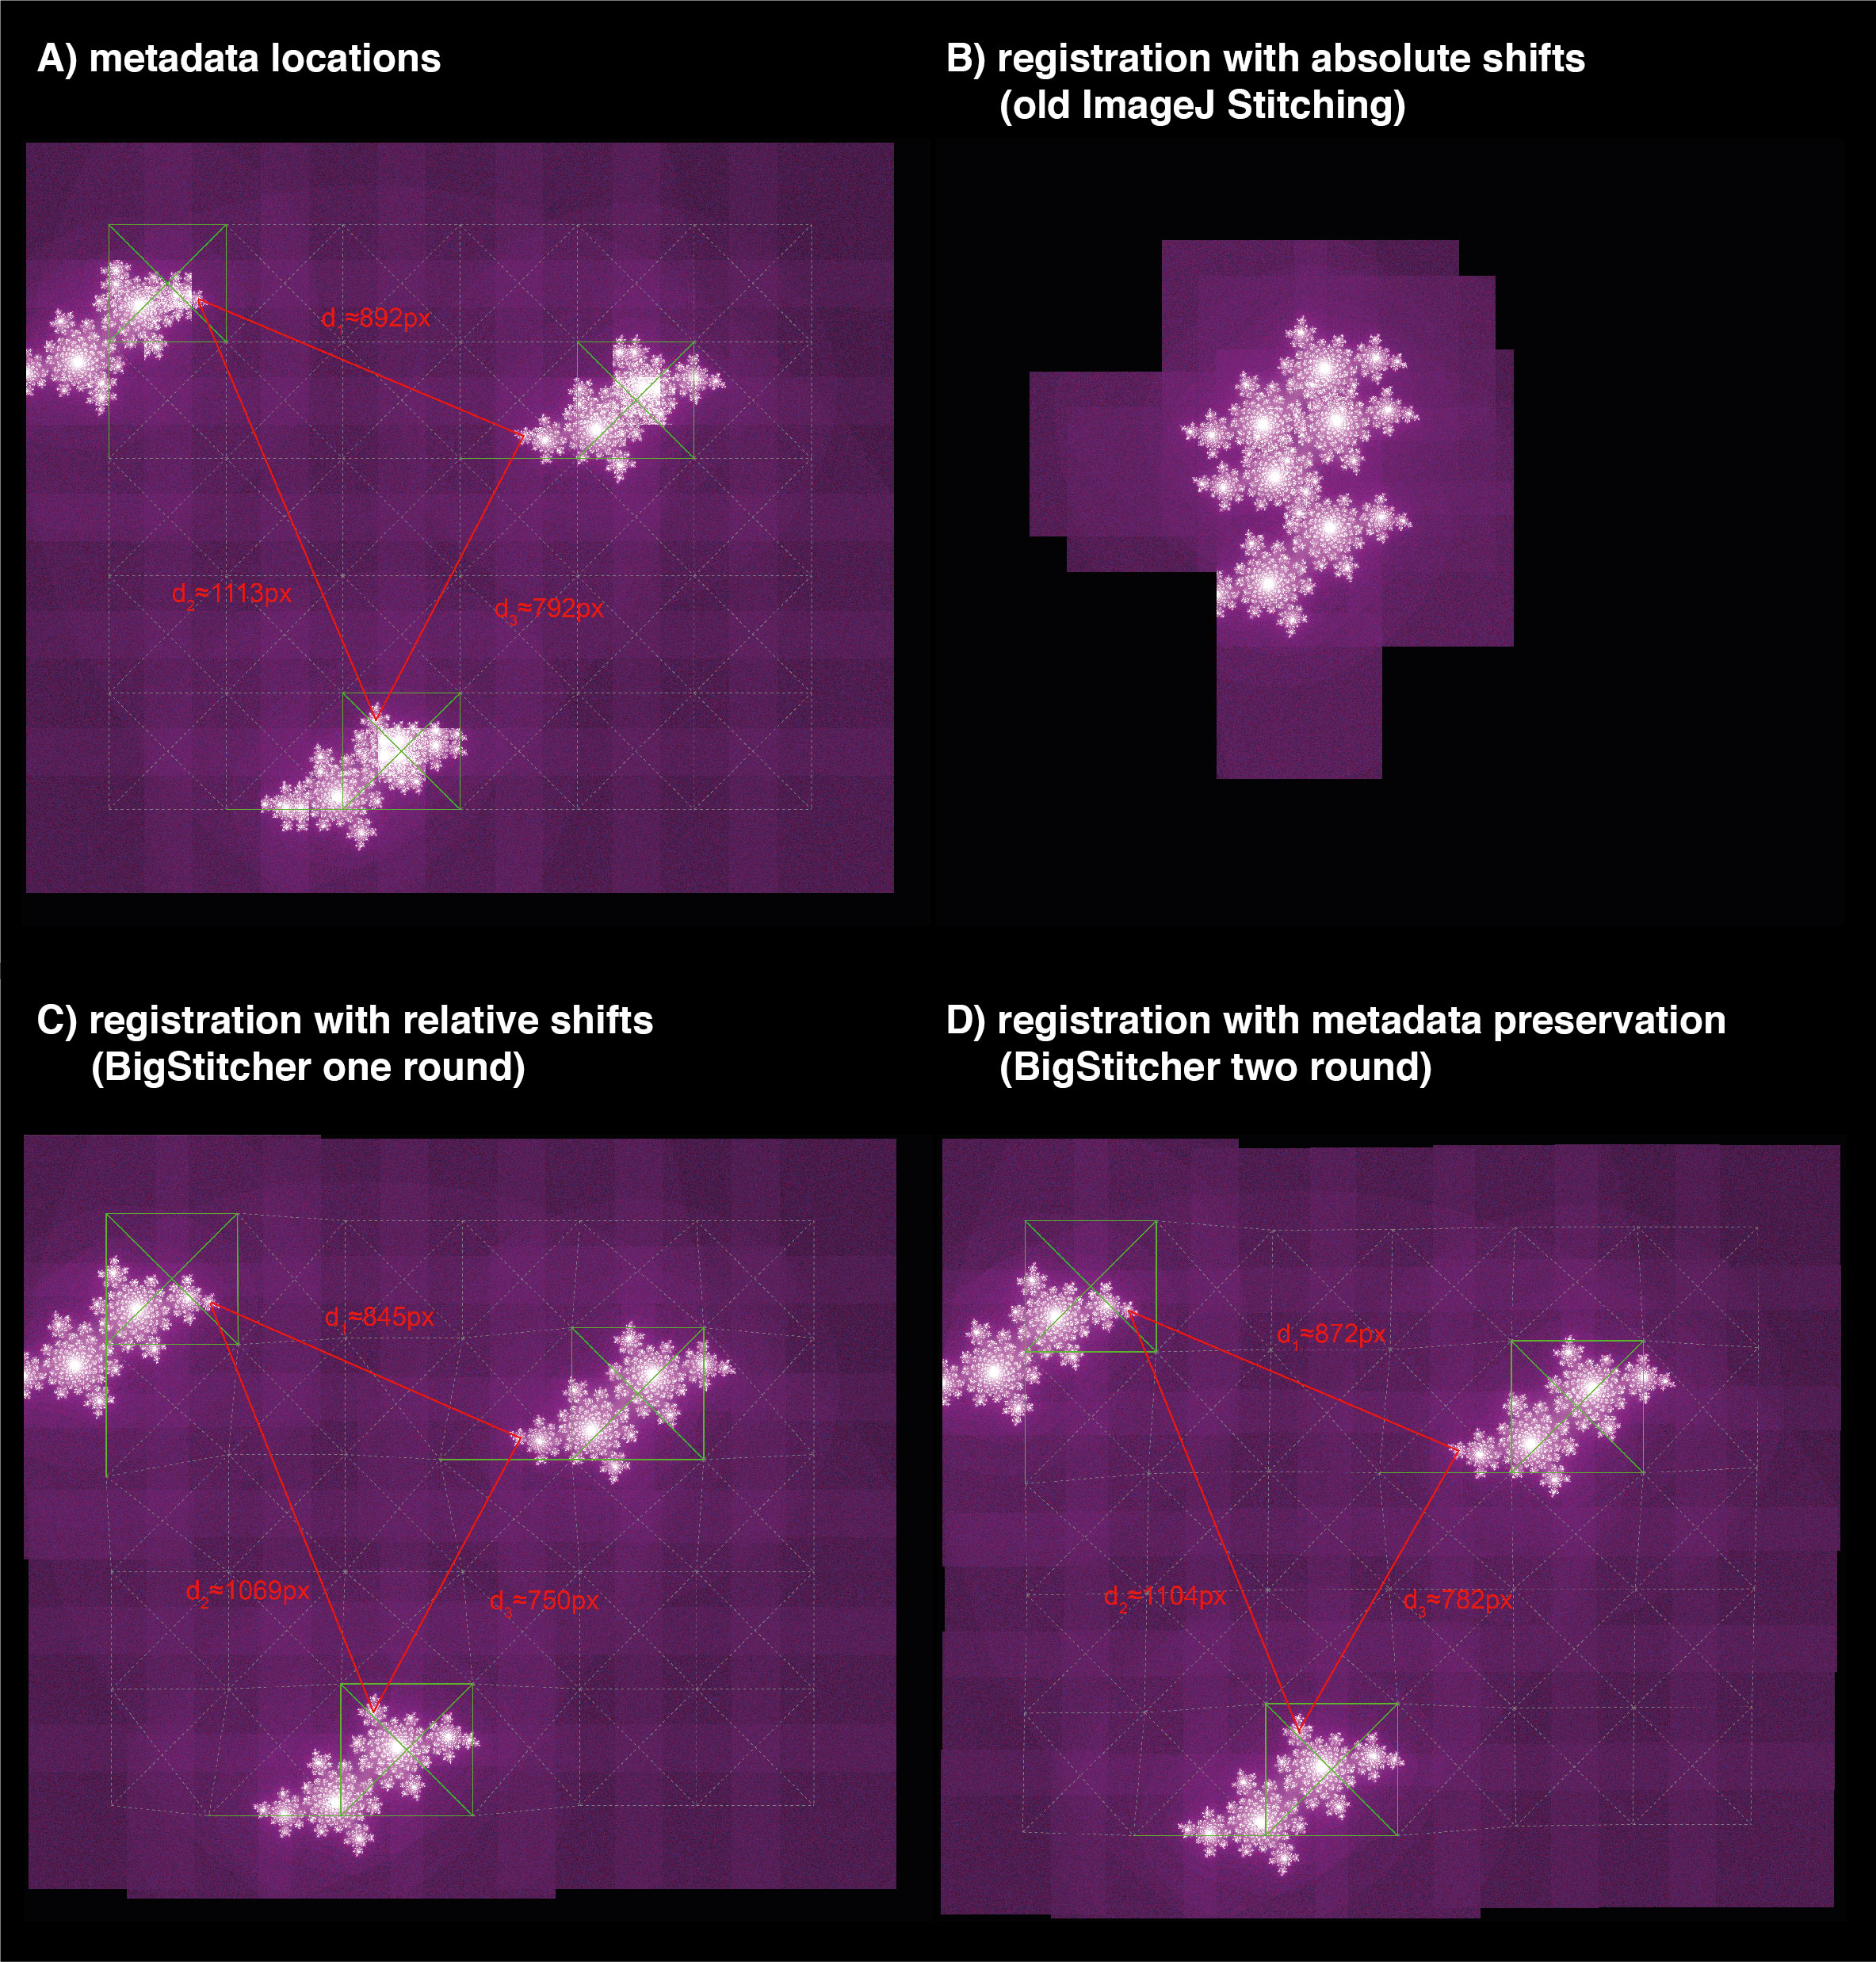
\includegraphics[width=0.82\textwidth]{fig-globalopt.jpg}}
\vspace{2.0mm}
\caption{\hspace{-0.5mm} \emph{Global optimization of pairwise registration in sparse datasets connected by "empty tiles" (noise only) .} \textbf{(A)} Simulation of a tiled image dataset with sparse objects: tiled images of multiple translated Julia fractals moved to a grid according to approximate metadata (with too high overlap). Centers of images for which pairwise shifts can be determined via phase correlation are connected by green lines, whereas centers of neighboring tiles for which no meaningful shift can be calculated are linked by dashed grey lines. Manually measured distances between distinct points in the three fractals are shown in red. \textbf{(B)} performing global optimization with \emph{absolute shifts} (as it is done BigStitcher's predecessor, the ImageJ Stitching plugin) will correctly align images within connected components of the link graph but place all fractals close to the origin. \textbf{(C)} by using \emph{relative shifts}, BigStitcher will leave disconnected objects at their initial location while still aligning within connected components. \textbf{(D)} as registrations are not propagated between unconnected tiles, distances between neighboring objects might change. By running a second round of optimization to align connected components according to metadata shifts and applying the results to the in-component registrations, distances between neighboring objects are preserved as-good-as-possible. \textbf{(A-D)} Two-round global optimization as illustrated in this figure is a feature supported by BigStitcher, which has been applied to all datasets used in this publication. Especially the dataset shown in \textbf{Fig. 1d,e and Fig. 3d} profits from it since it contains empty tiles.
}
\label{fig:sup-fig-globalopt}
\end{figure*}

\pagebreak

\subsection*{SUPPLEMENTARY FIGURE 11: Pairwise registration by phase correlation}
\vspace{-2mm}
\begin{figure*}[h!]
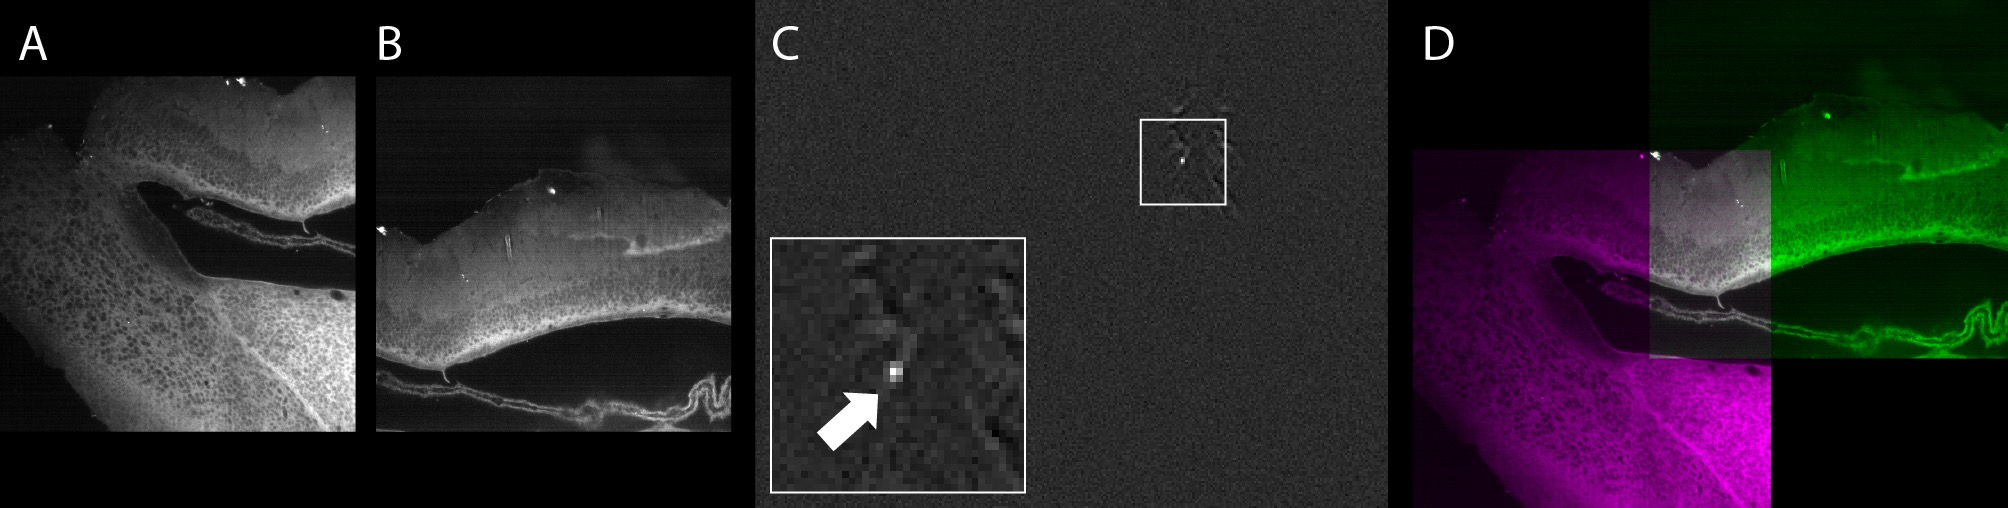
\includegraphics[width=\textwidth]{fig-stitching.jpg}
\vspace{-2.0mm}
\caption{\hspace{-0.5mm} \emph{Pairwise registration by phase correlation}. \textbf{(A,B)} Central slices of image stacks from a tiled acquisition (non-regular tiling) of a cleared adult mouse hypothalamus. \textbf{(C)} Phase correlation matrix (PCM) calculated from the two images shows a single, distinct peak above nearly constant background. The peak location corresponds to the relative translation $t$ of both tiles. \textbf{(D)} Central slice through the images aligned according to $t$, as displayed in interactively during the reconstruction process. \textbf{(A-D)} The pairwise registration using phase correlation was used as a first step in the alignment of all cleared and expanded samples used in this publication (\textbf{Suppl. Table 1}).
}
\label{fig:sup-fig-stitching}
\end{figure*}

\pagebreak

\subsection*{SUPPLEMENTARY FIGURE 12: Downsampling with different SNR}
\vspace{-2mm}
\begin{figure*}[h!]
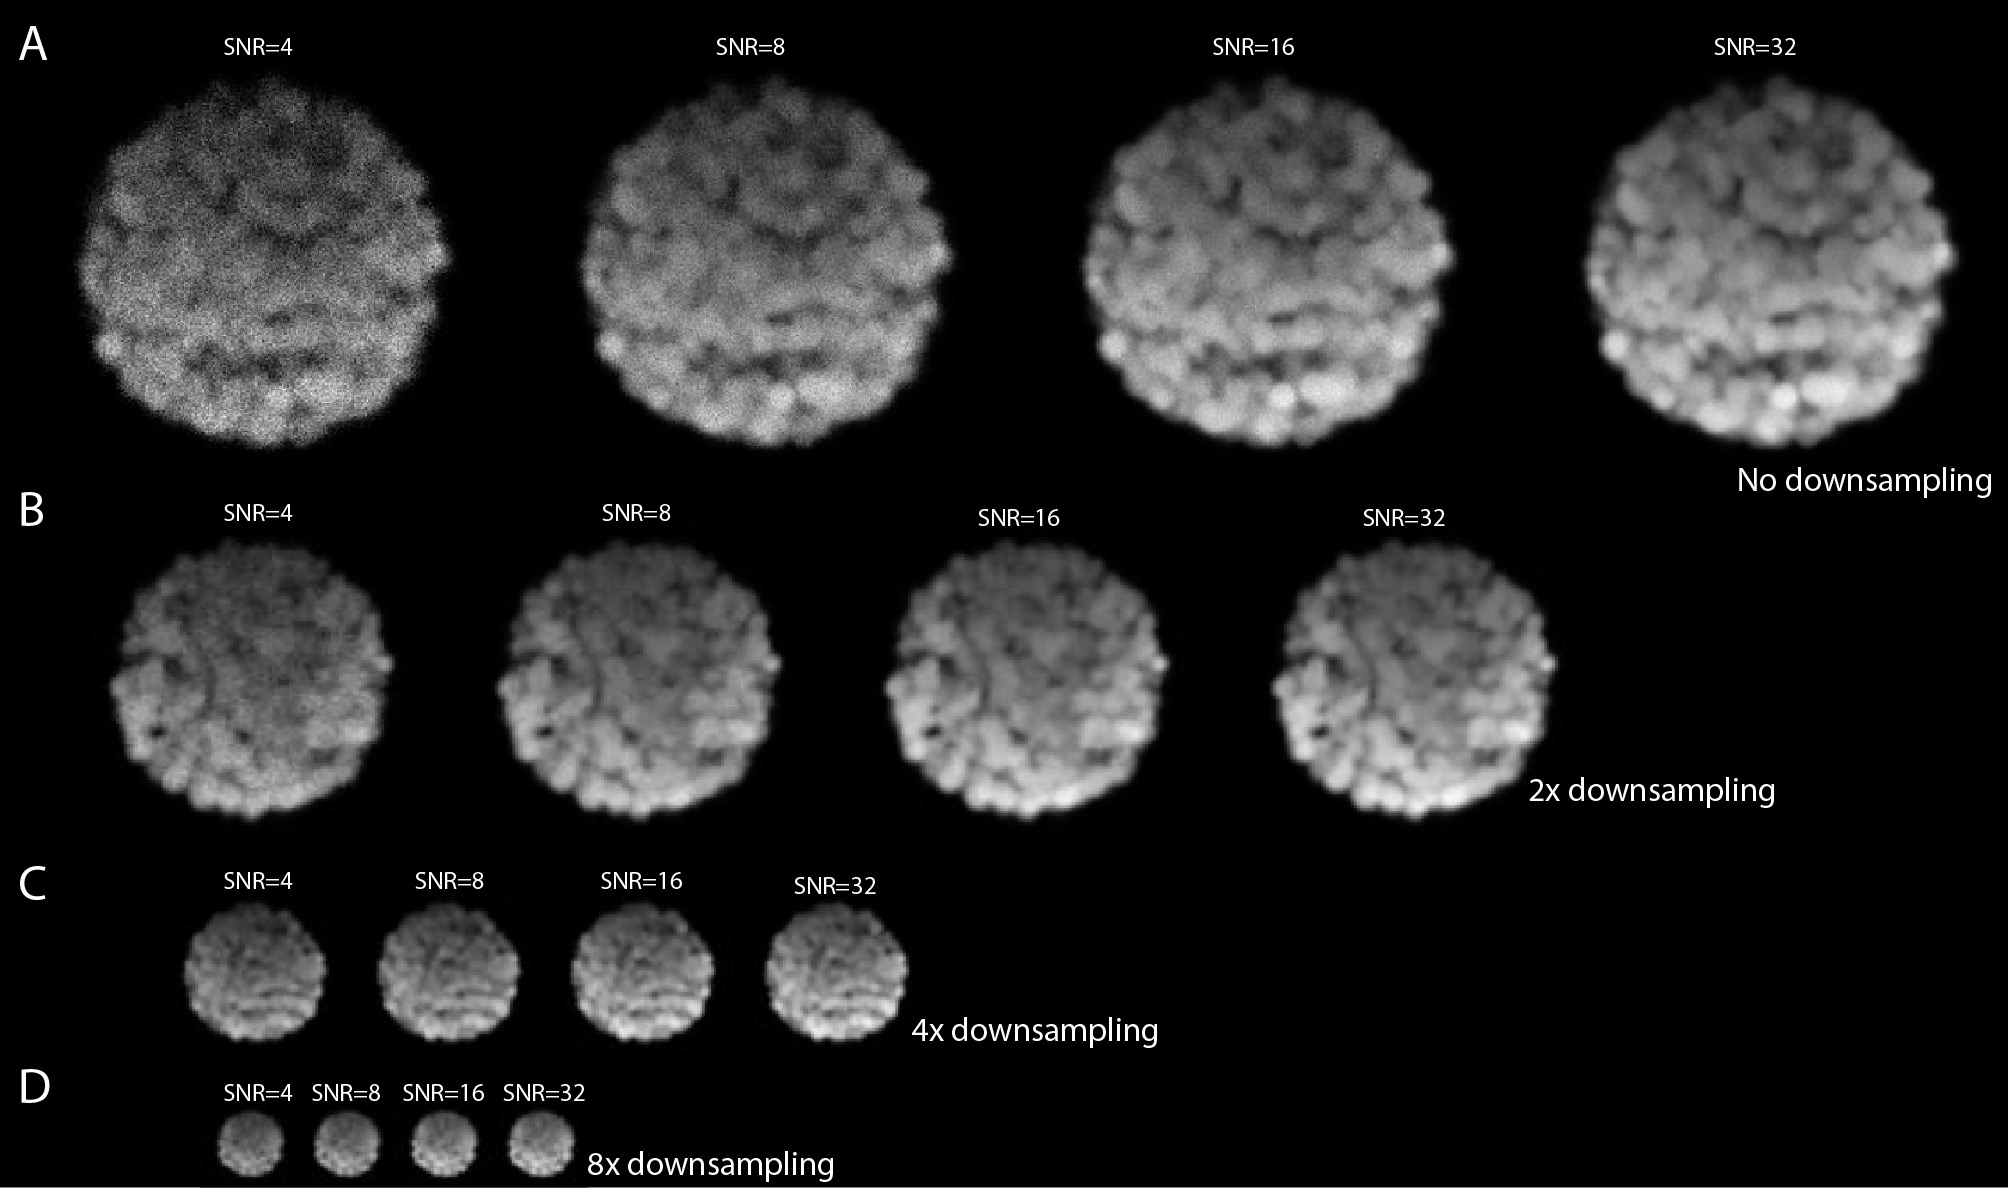
\includegraphics[width=\textwidth]{fig-downsampling.jpg}
\vspace{-2.0mm}
\caption{\hspace{-0.5mm} \emph{Effects of downsampling on simulated data with different SNR.} \textbf{(A)} Simulated image stacks of spheroid-like objects deteriorated by anisotropic sampling, light attenuation, convolution with an anisotropic PSF, and pixel intensity generation using Poisson processes to archive desired signal-to-noise-ratios (SNRs). A central slice through 3d volumes is shown. \textbf{(B,C,D)} Effects of downsampling on the simulated images. The effects of Poisson Shot Noise are gradually reduced by the blurring of increasing downsampling. \textbf{(A)} For quantification of the alignment quality using these simulations, 300 independent simulations were run for each combination of SNR and downsampling (see \textbf{Supp. Fig. \ref{fig:sup-fig-downsampling-statistics-0} -- \ref{fig:sup-fig-downsampling-statistics-2}}).
}
\label{fig:sup-fig-downsampling}
\end{figure*}

\pagebreak

\subsection*{SUPPLEMENTARY FIGURE 13: Downsampling statistics 1}
\vspace{1mm}
\begin{figure*}[h!]
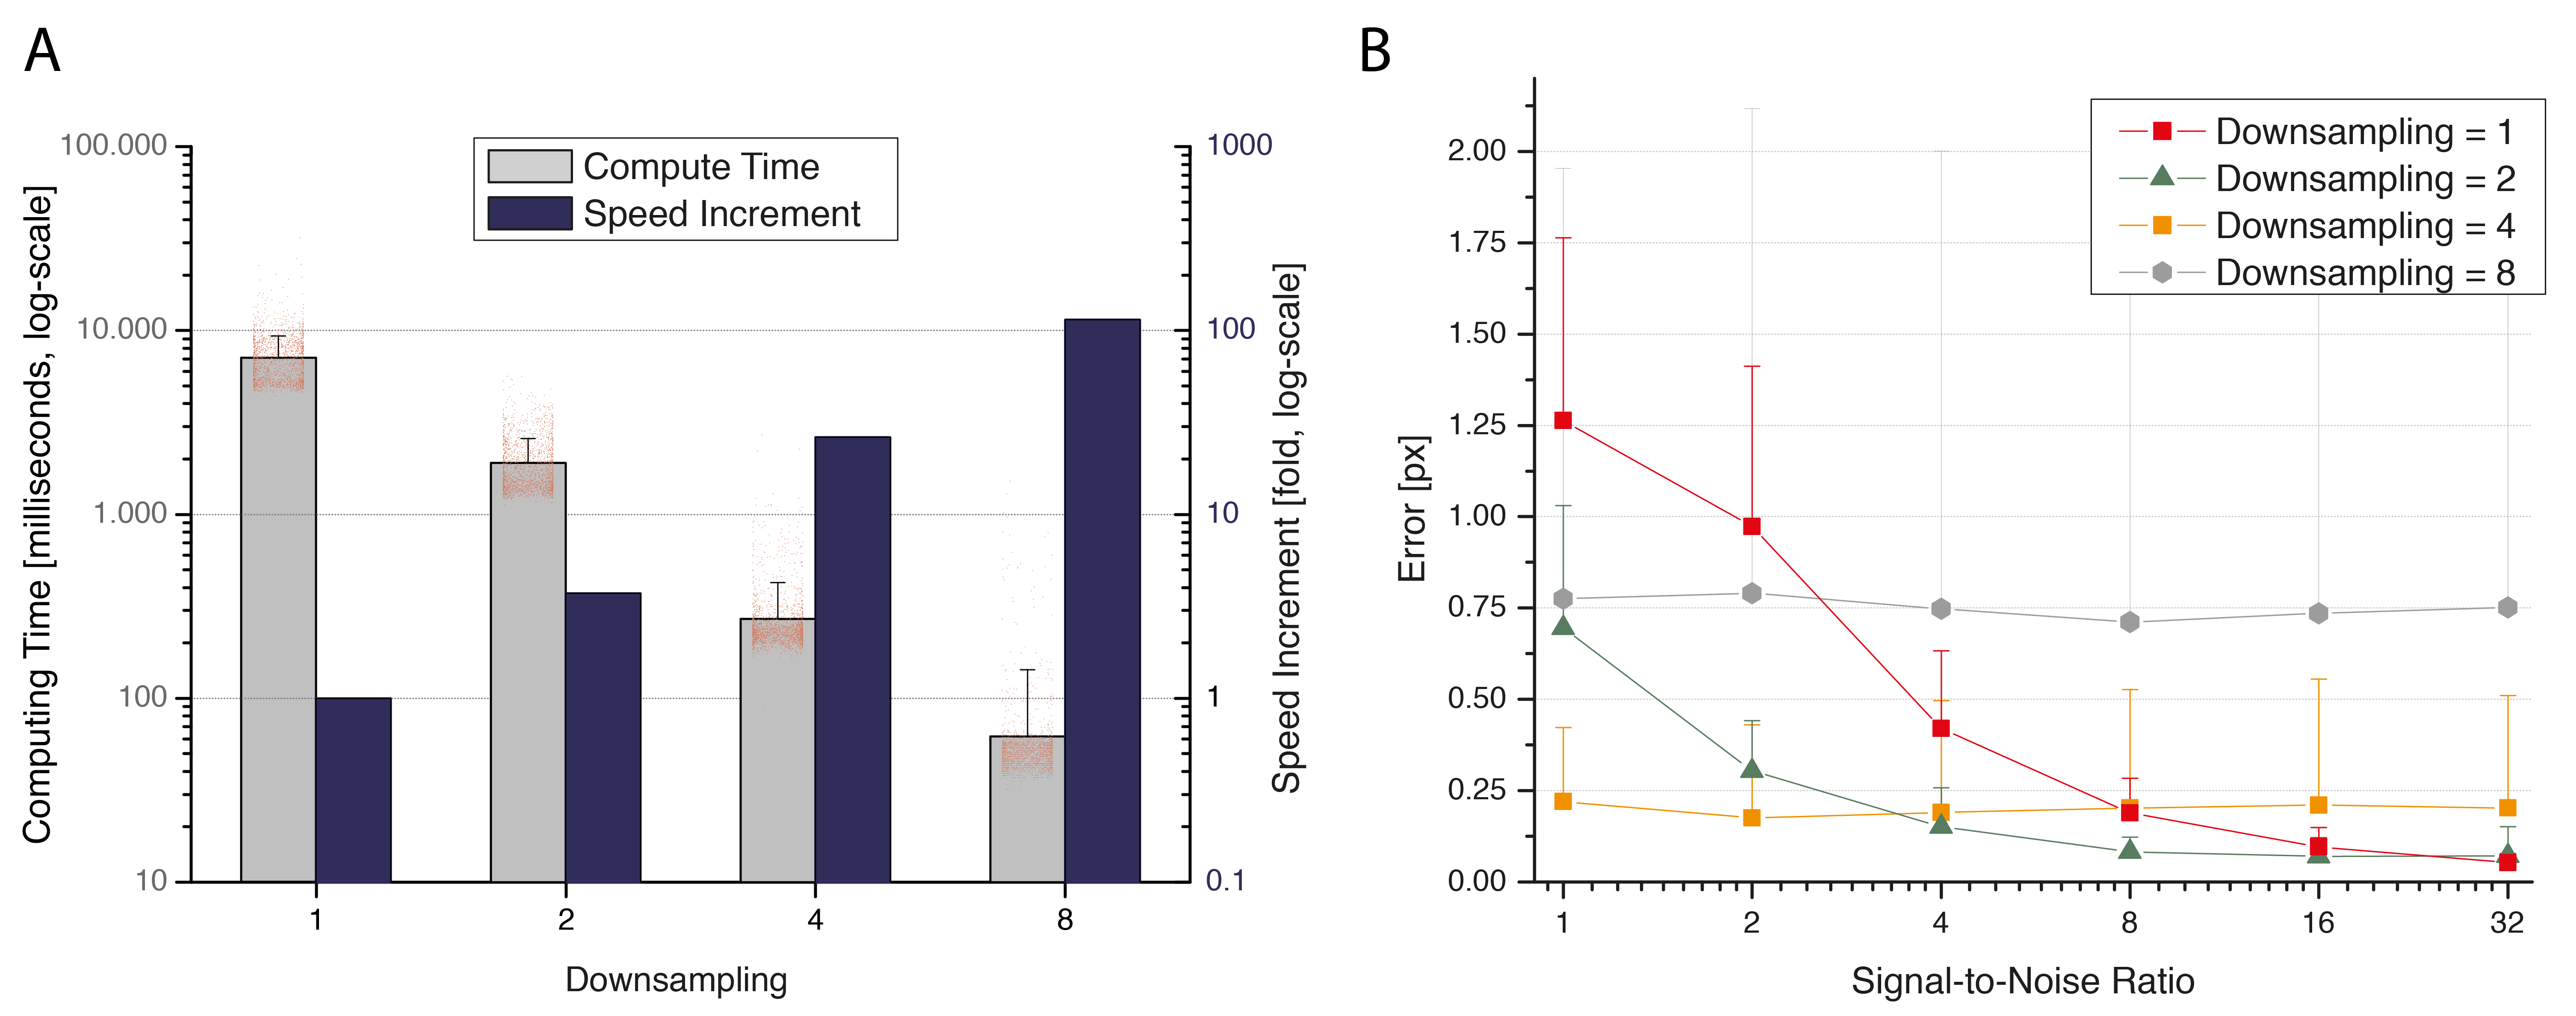
\includegraphics[width=\textwidth]{fig-downsampling-statistics-0.png}
\vspace{-2.0mm}
\caption{\hspace{-0.5mm} \emph{Processing times and overall errors.} \textbf{(A)} Processing times for sub-pixel precise identification of overlap between simulation spheroids. With increasing downsampling, the computation time drops significantly. Red dots show individual measurements, note the log-scale. Average (StDev) of computing time is 7122 (2224) msec, 1910 (681) msec, 271 (155) msec, and 62 (80) msec for downsampling 1, 2, 4 and 8, respectively. The speed increments are computed as the ratio of the average compute times, i.e. 1$\times$, $\sim$4$\times$, $\sim$26$\times$, and $\sim$115$\times$, respectively. Compute times were measured in a single thread on a Intel~Xeon E5-2640~v4. \textbf{(B)} Average errors including their standard deviation for all combinations of SNR and downsampling. \textbf{(A,B)} All errors are in units of the input images (no downsampling). For each combination of SNR and downsampling 300 independent simulations were run to compute the values.
}
\label{fig:sup-fig-downsampling-statistics-0}
\end{figure*}

\subsection*{SUPPLEMENTARY FIGURE 14: Downsampling statistics 2}
\vspace{1mm}
\begin{figure*}[h!]
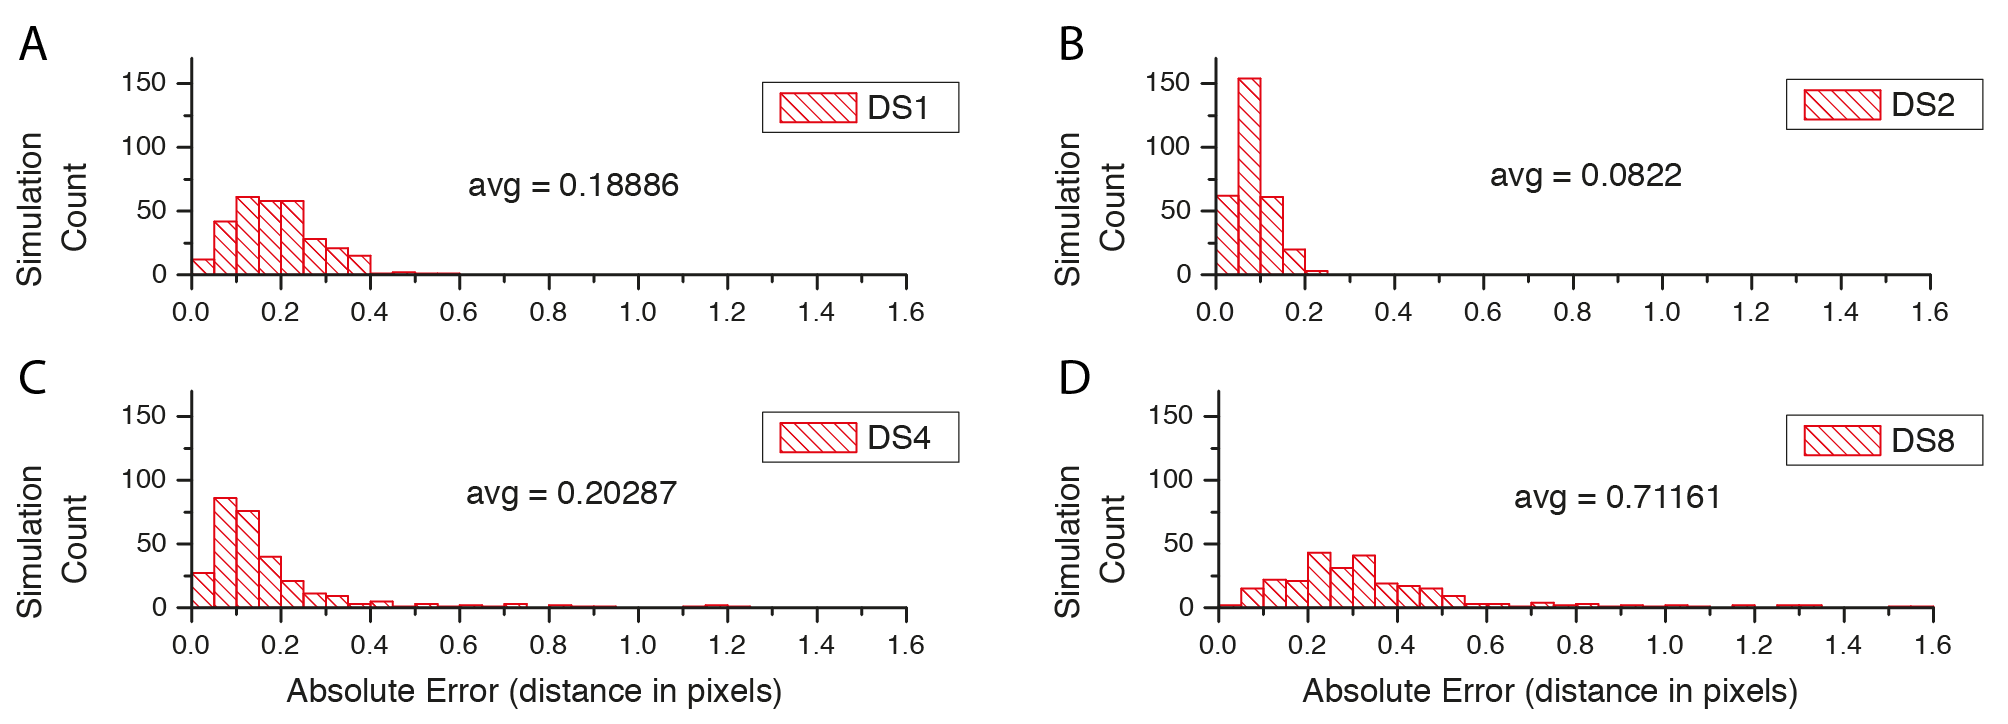
\includegraphics[width=\textwidth]{fig-downsampling-statistics-1.png}
\vspace{-2.0mm}
\caption{\hspace{-0.5mm} \emph{Errors for different downsamplings at SNR=8.} \textbf{(A-D)} Histograms showing the distributions of error of the simulations. Errors initially decrease due to the smoothing effect of the downsampling. All errors are in pixel units of the original resolution (DS1). Each histogram consists of 300 independent simulations.
}
\label{fig:sup-fig-downsampling-statistics-1}
\end{figure*}

\pagebreak

\subsection*{SUPPLEMENTARY FIGURE 15: Downsampling statistics 3}
\vspace{1mm}
\begin{figure*}[h!]
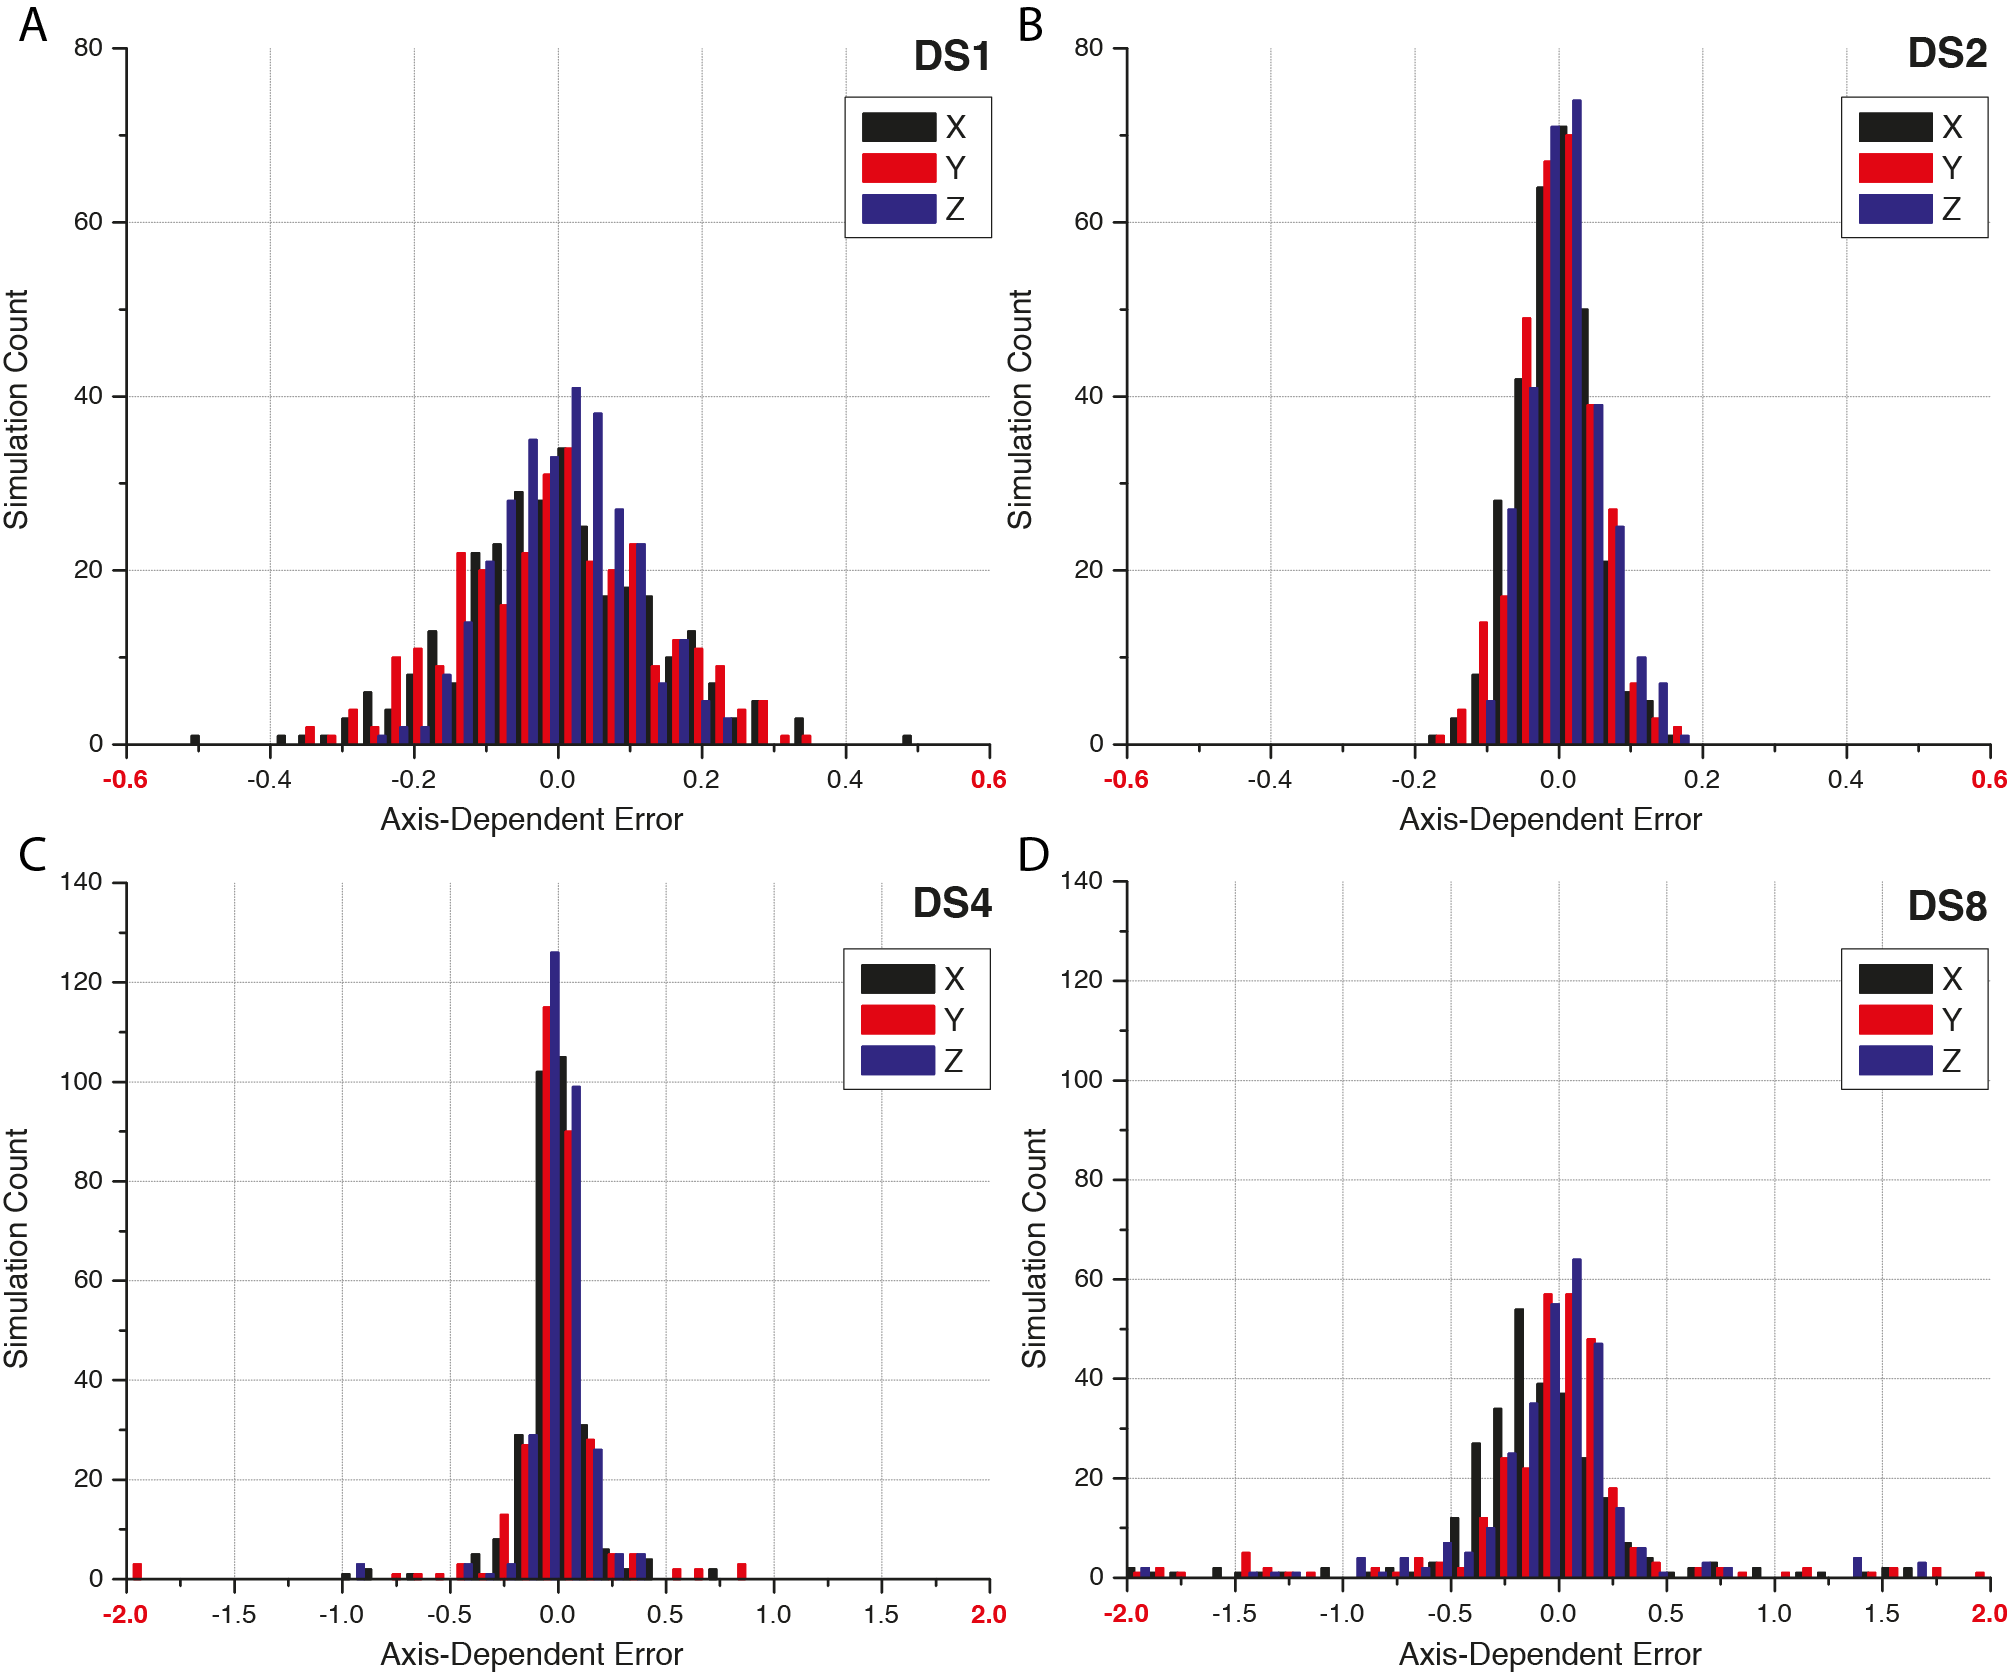
\includegraphics[width=\textwidth]{fig-downsampling-statistics-2.png}
\vspace{-2.0mm}
\caption{\hspace{-0.5mm} \emph{Absolute distance errors at SNR=8.} \textbf{(A-D)}  Histograms showing the absolute distances between computed and known shift between two simulated spheroids, split by dimension. It illustrates a normal distribution of the error made during the pairwise phase correlation. All errors are in pixel units of the original resolution (DS1). Each histogram consists of 300 independent simulations.
}
\label{fig:sup-fig-downsampling-statistics-2}
\end{figure*}

\pagebreak

\subsection*{SUPPLEMENTARY FIGURE 16: Interactive inspection and curation of pairwise links}
\vspace{1mm}
\begin{figure*}[h!]
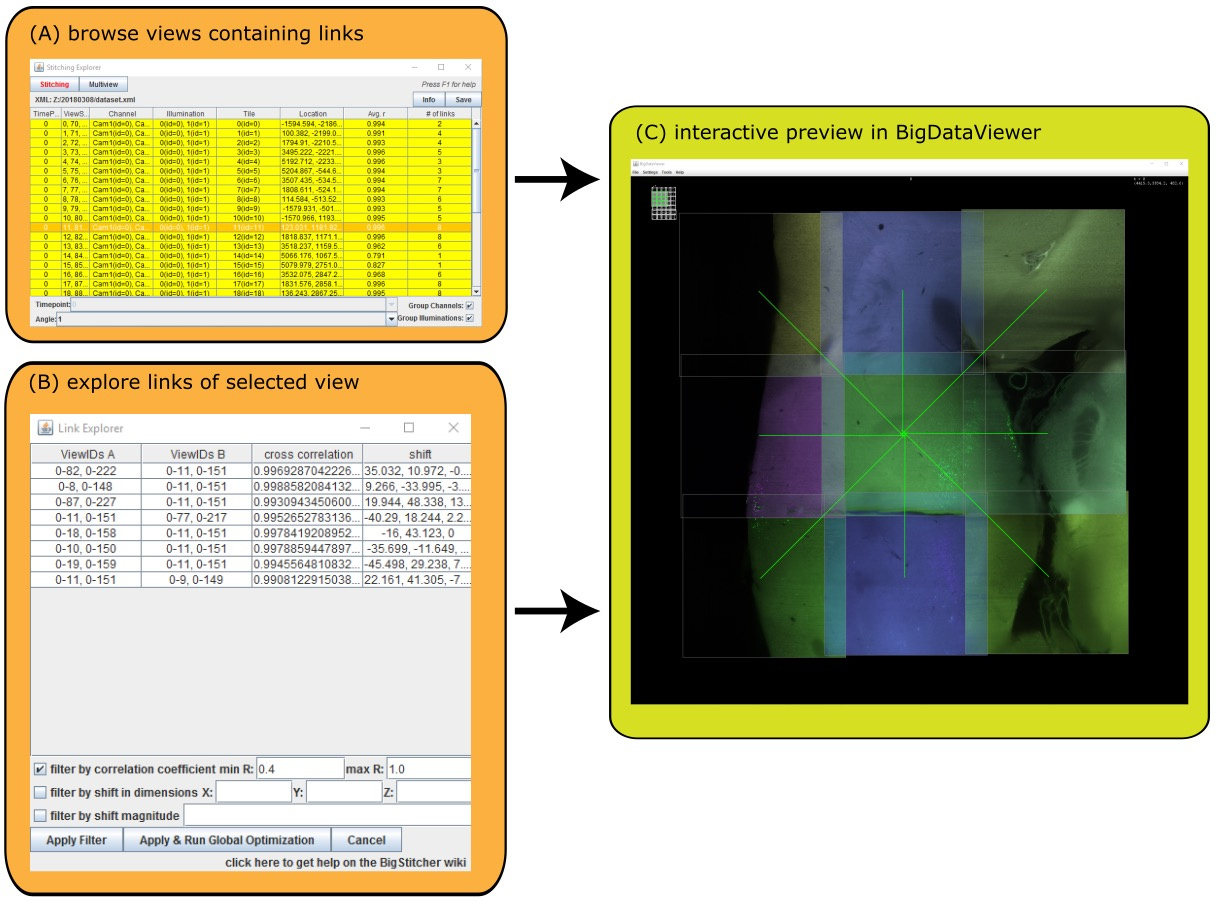
\includegraphics[width=\textwidth]{Supp-Link-Explorer.jpg}
\vspace{-2.0mm}
\caption{\hspace{-0.5mm} \emph{Interactive visualization of links in the link explorer.} The BigStitcher GUI offers to explore and modify calculated links between corresponding tiles in the link explorer menu. \textbf{(A)} tiles containing links are displayed in yellow and can be selected. \textbf{(B)} display corresponding tiles of the selected view. Single links can be removed manually or through available filtering options. \textbf{(C)} corresponding links of the selected view are displayed in real-time in the BigDataViewer.
}
\label{fig:sup-fig-link-explorer}
\end{figure*}

\pagebreak

\subsection*{\red{SUPPLEMENTARY FIGURE 17: Quantification of image registration quality}}
\vspace{-2mm}
\begin{figure*}[h!]
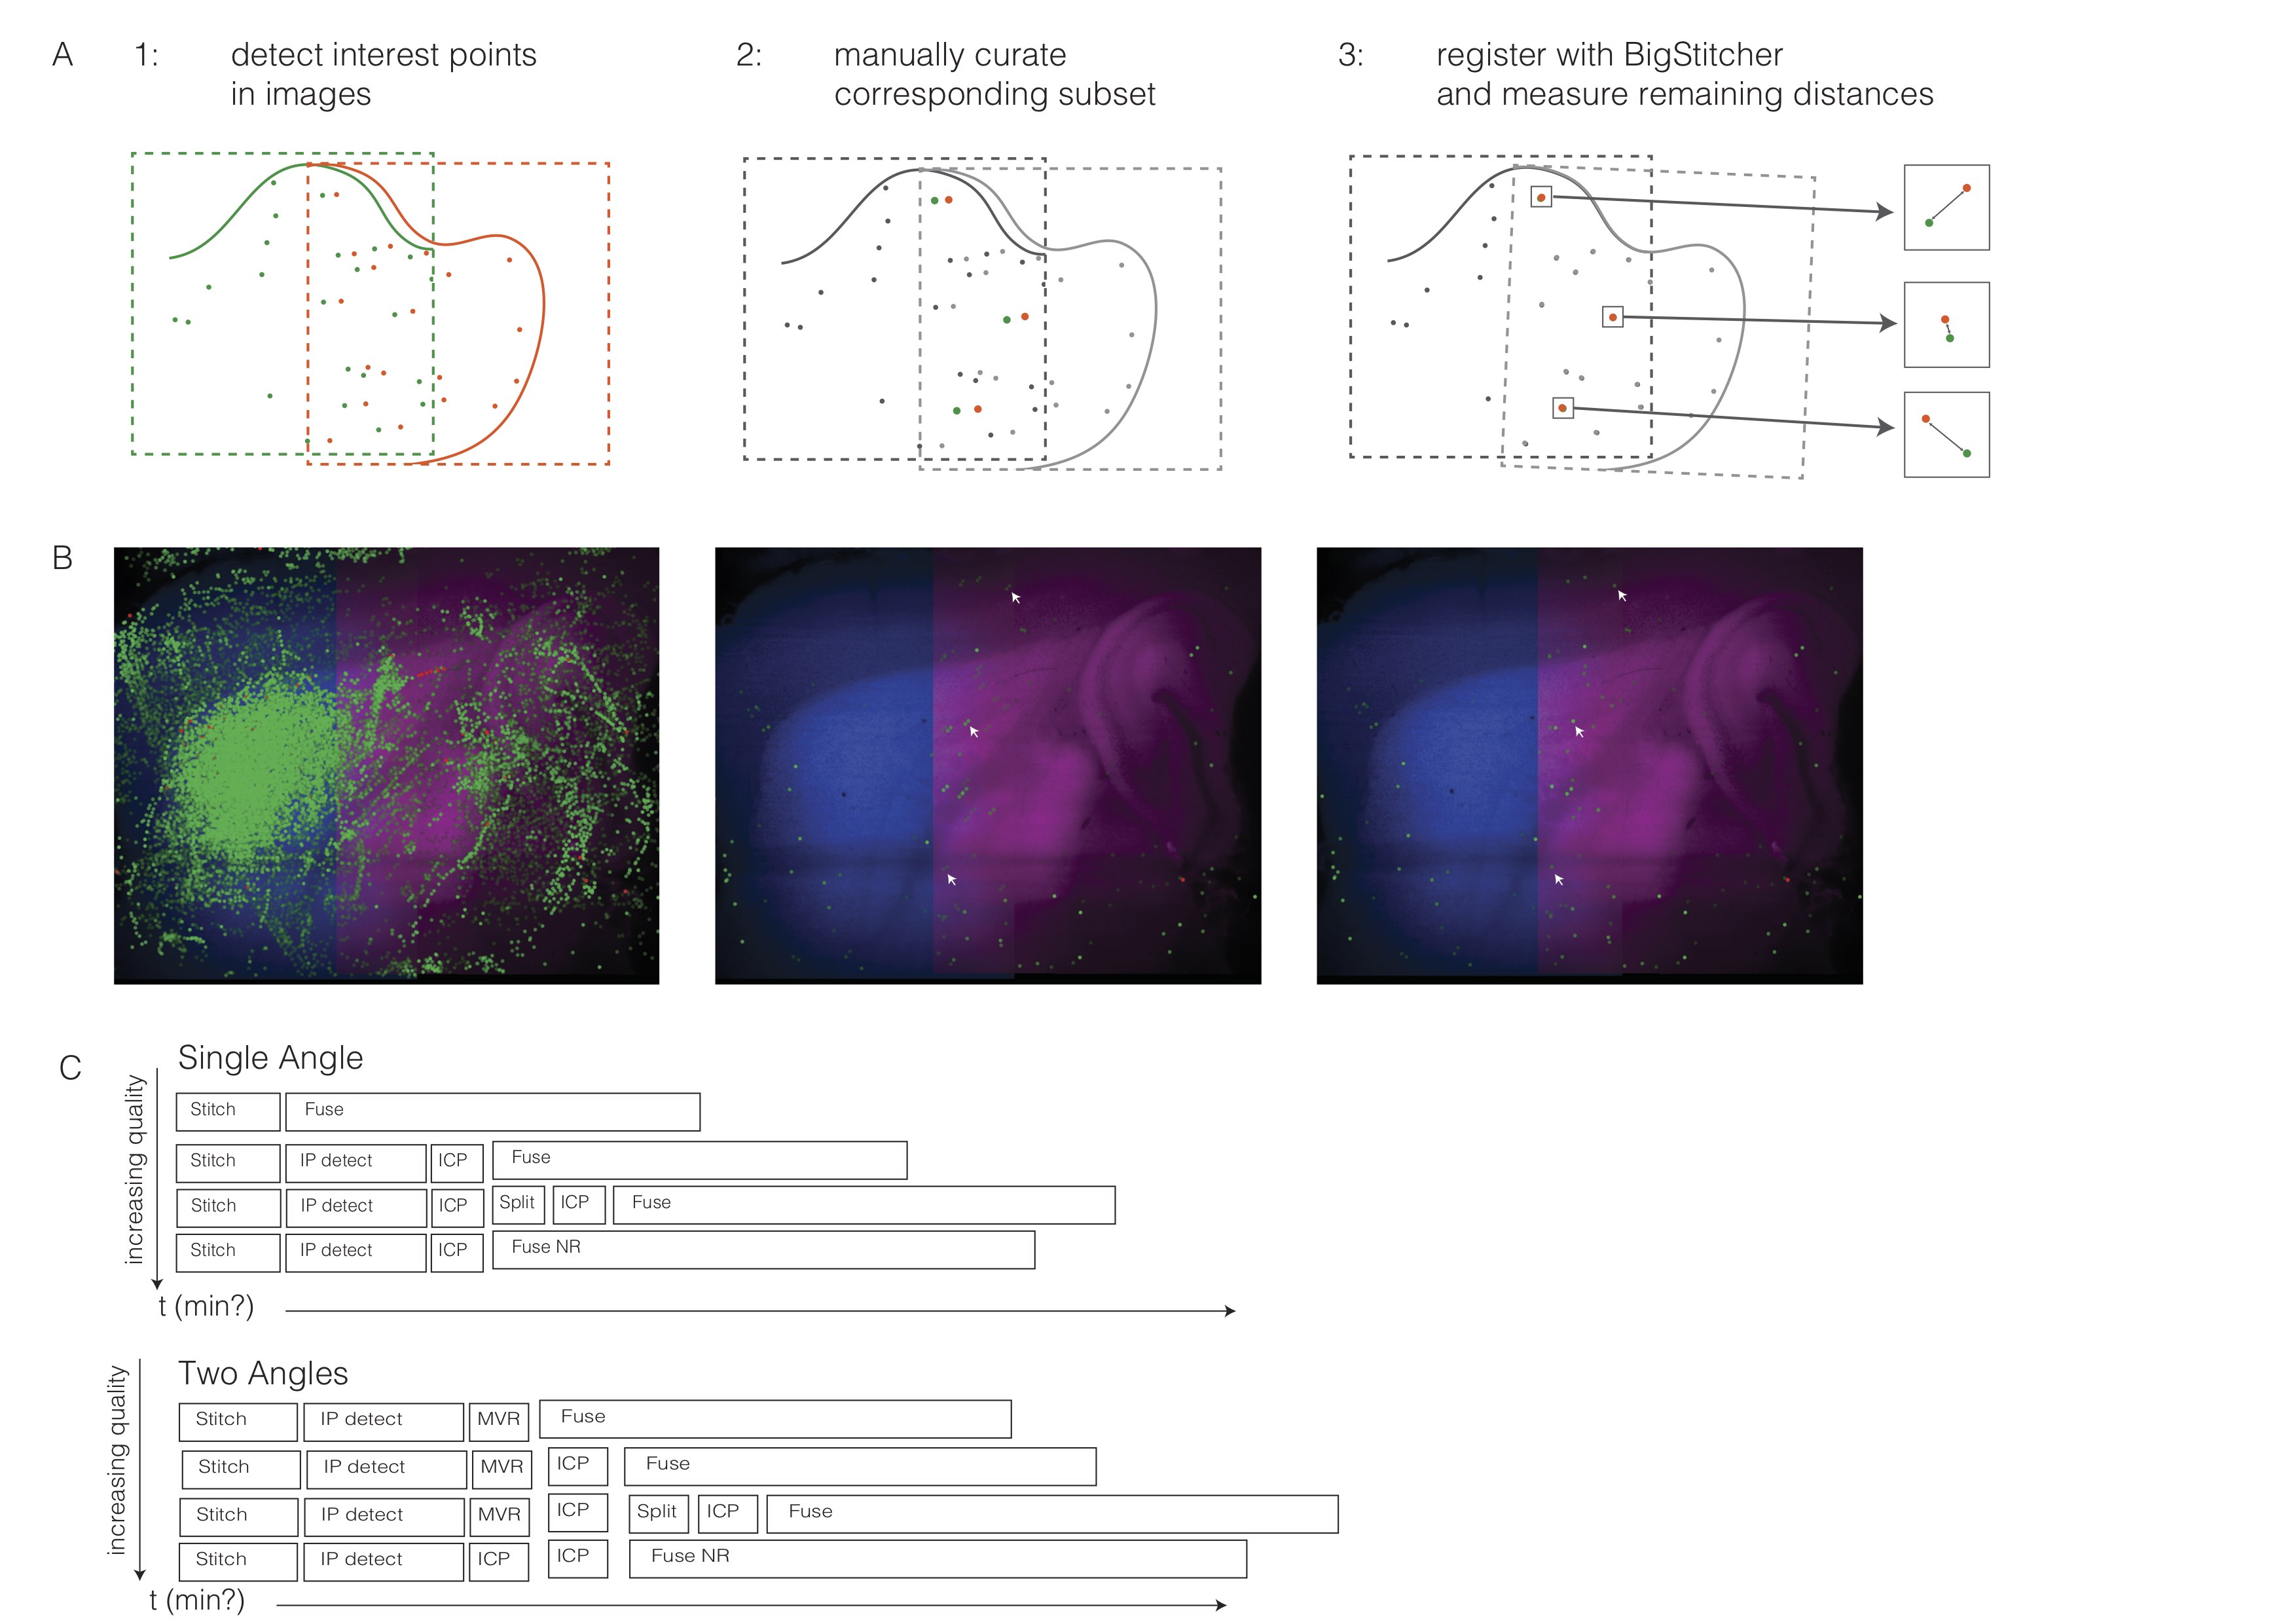
\includegraphics[width=\textwidth]{bigstitcher_registrationquality.jpg}
\vspace{-4.0mm}
\caption{\hspace{-0.5mm} \red{\emph{Quantification of Image Registration Quality.} A multi-view, dual-illumination, multi-tile dataset specifically acquired for verification purposes was used to quantify the registration error (see \textbf{Online Methods}, \textbf{Fig.2k-m}, and \textbf{Supp. Fig. 2}). \textbf{(A)}: Schematic description of the quantification process for registration accuracy. Interest points are first automatically detected in all images of the dataset (1). Of those, a subset of truly corresponding points interest points was selected for each pair of images (2). After registration with BigStitcher using various transformation models (translation, affine, split-affine, non-rigid), the remaining distance between the manually curated point pairs is used as a measure of registration error (3), actual errors are shown in \textbf{Fig. 2m}. \textbf{(B)} All interest points detected in two images of the example dataset overlaid on a slice view (left), manually selected corresponding points (middle, note the "doubling" of the paired points as they are not yet aligned, arrows indicate examples) and the same points after registration (right). \textbf{(C)} Time required for registration (left) and fusion (right) of the dataset, for a single angle (top) or both angles (bottom). The single angle values are averages of both angles. Fusion was done at full resolution, preserving original data anisotropy. Multi-resolution pyramids of the images were computed beforehand. Processing was done on 2 Intel Xeon E5-2680v4 processors and 256GB RAM, data was loaded from SSDs in RAID0 configuration. This error quantification was performed only on this specifically acquired dataset.
}}
\label{fig:sup-fig-registration-quality}
\end{figure*}

\pagebreak

\subsection*{SUPPLEMENTARY FIGURE 18: Bounding-box definition}
\vspace{1mm}
\begin{figure*}[h!]
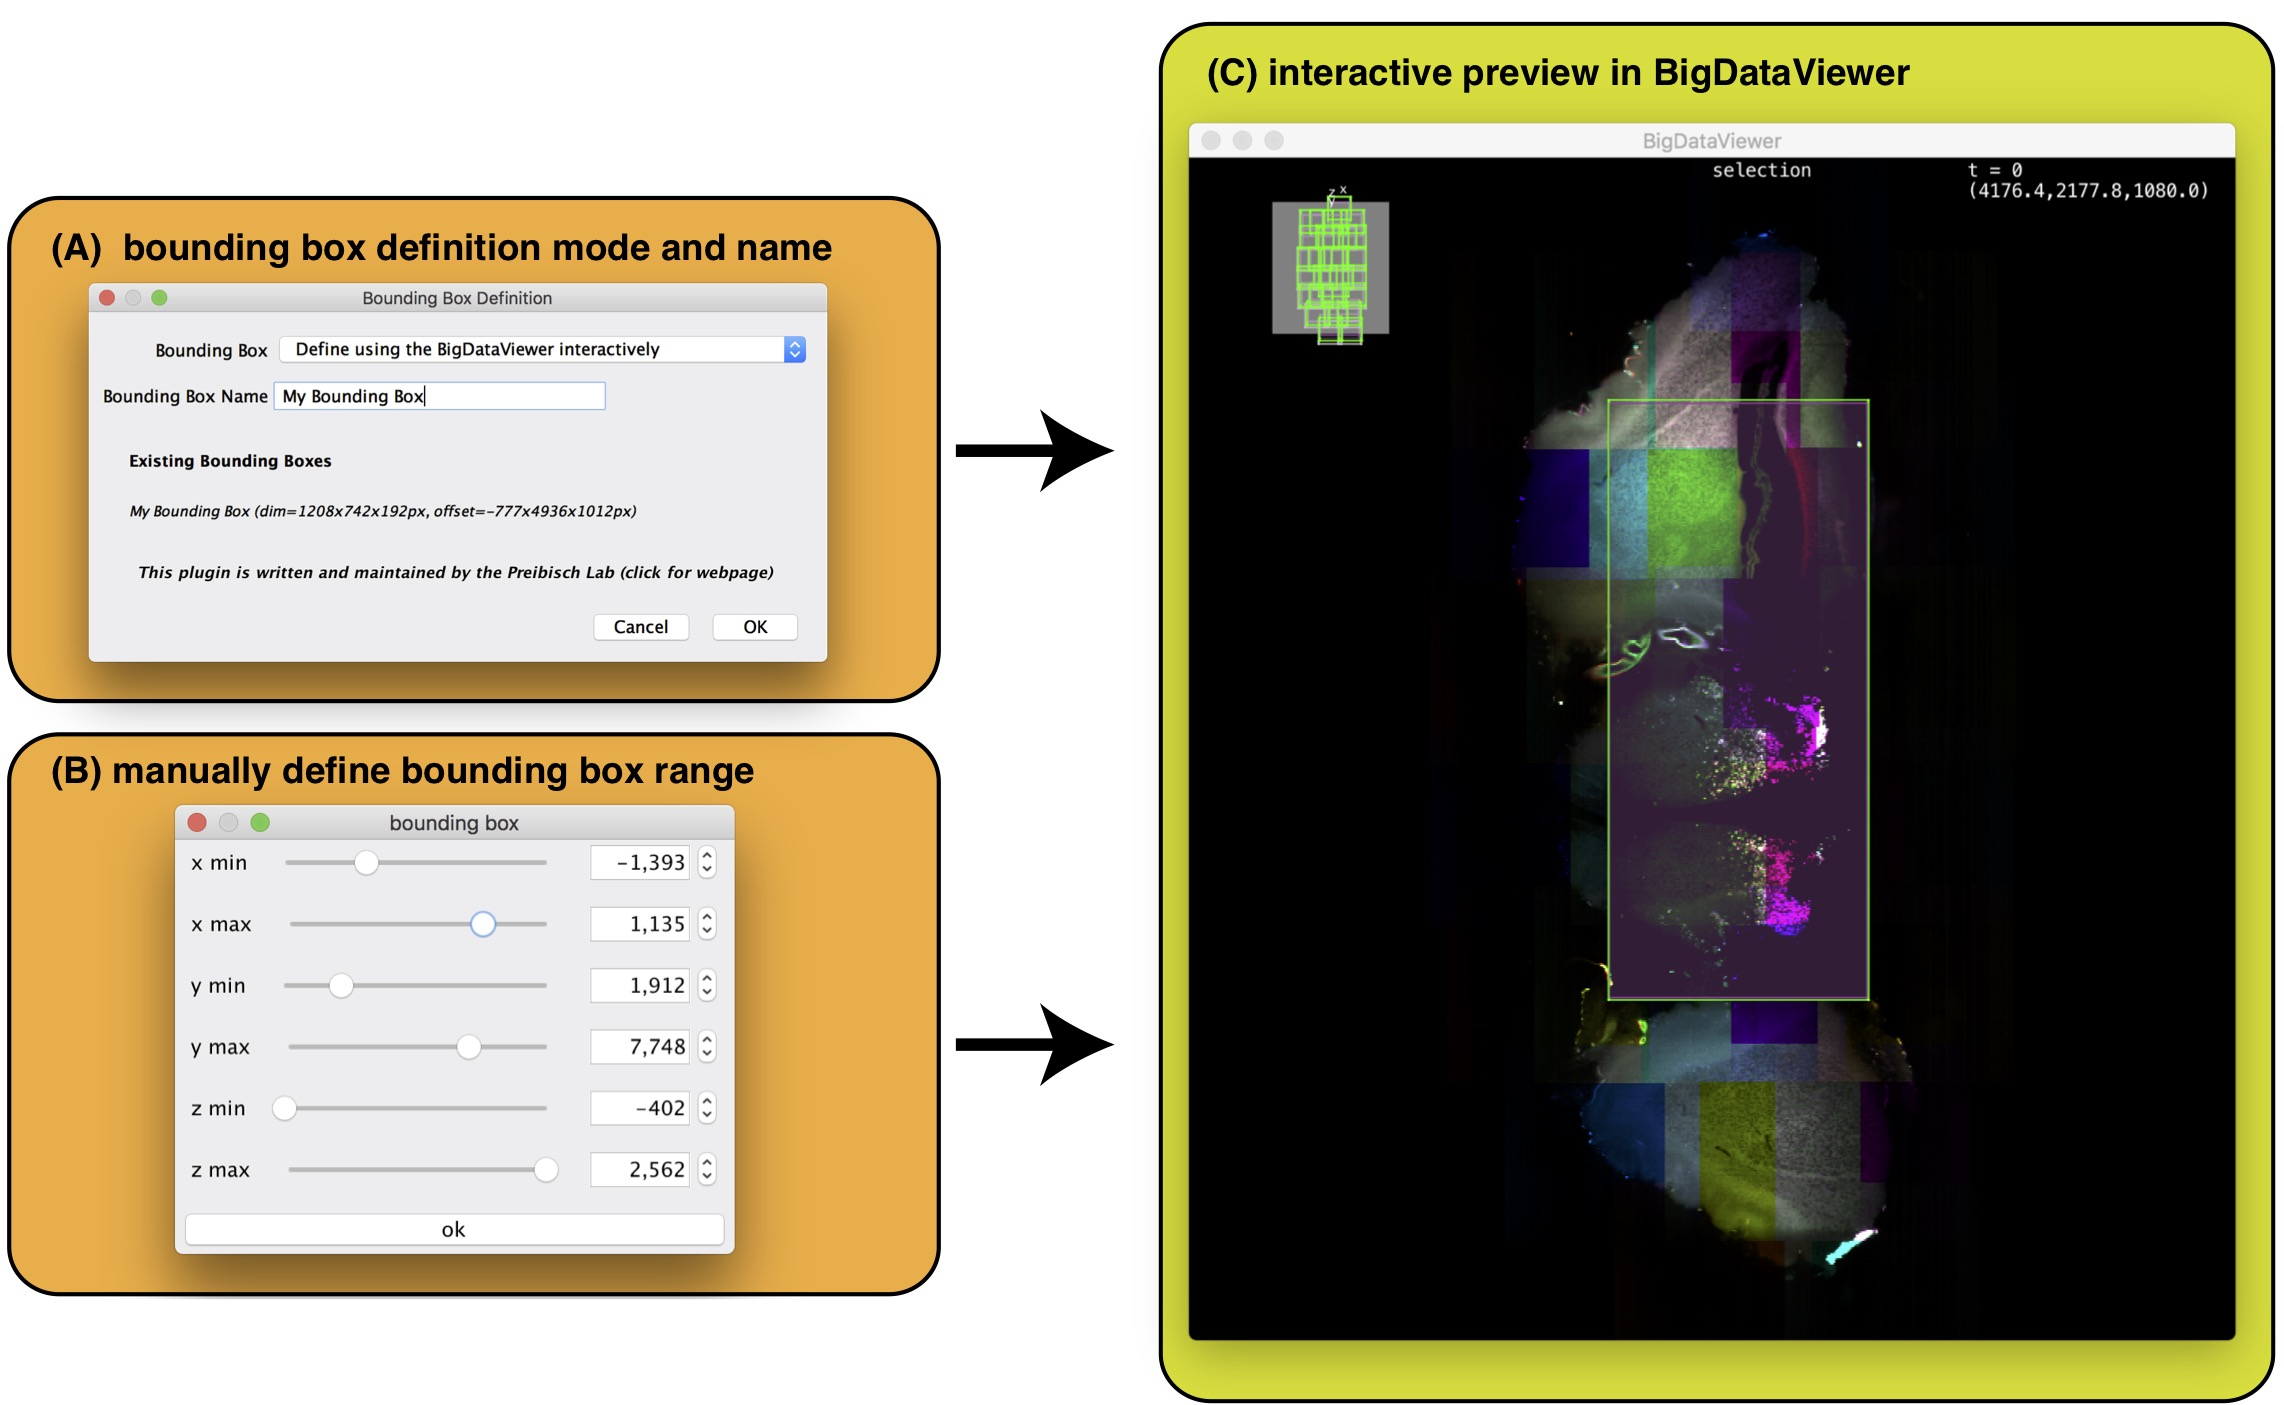
\includegraphics[width=\textwidth]{Supp-BB.jpg}
\vspace{-2.0mm}
\caption{\hspace{-0.5mm} \emph{Interactive definition of bounding boxes.} The BigStitcher GUI offers the possibility of defining or modifying regions of interest via the creation of bounding boxes. \textbf{(A)} Choose the method used to define a new bounding box. In this case the interactive mode is selected. \textbf{(B)} manually define the bounding box range \textbf{(C)} Preview the size of the specified bounding box in the BigDataViewer in real-time.
}
\label{fig:sup-fig-boundingbox}
\end{figure*}

\pagebreak

\subsection*{SUPPLEMENTARY FIGURE 19: Virtual fusion of large Image}
\vspace{1mm}
\begin{figure*}[h!]
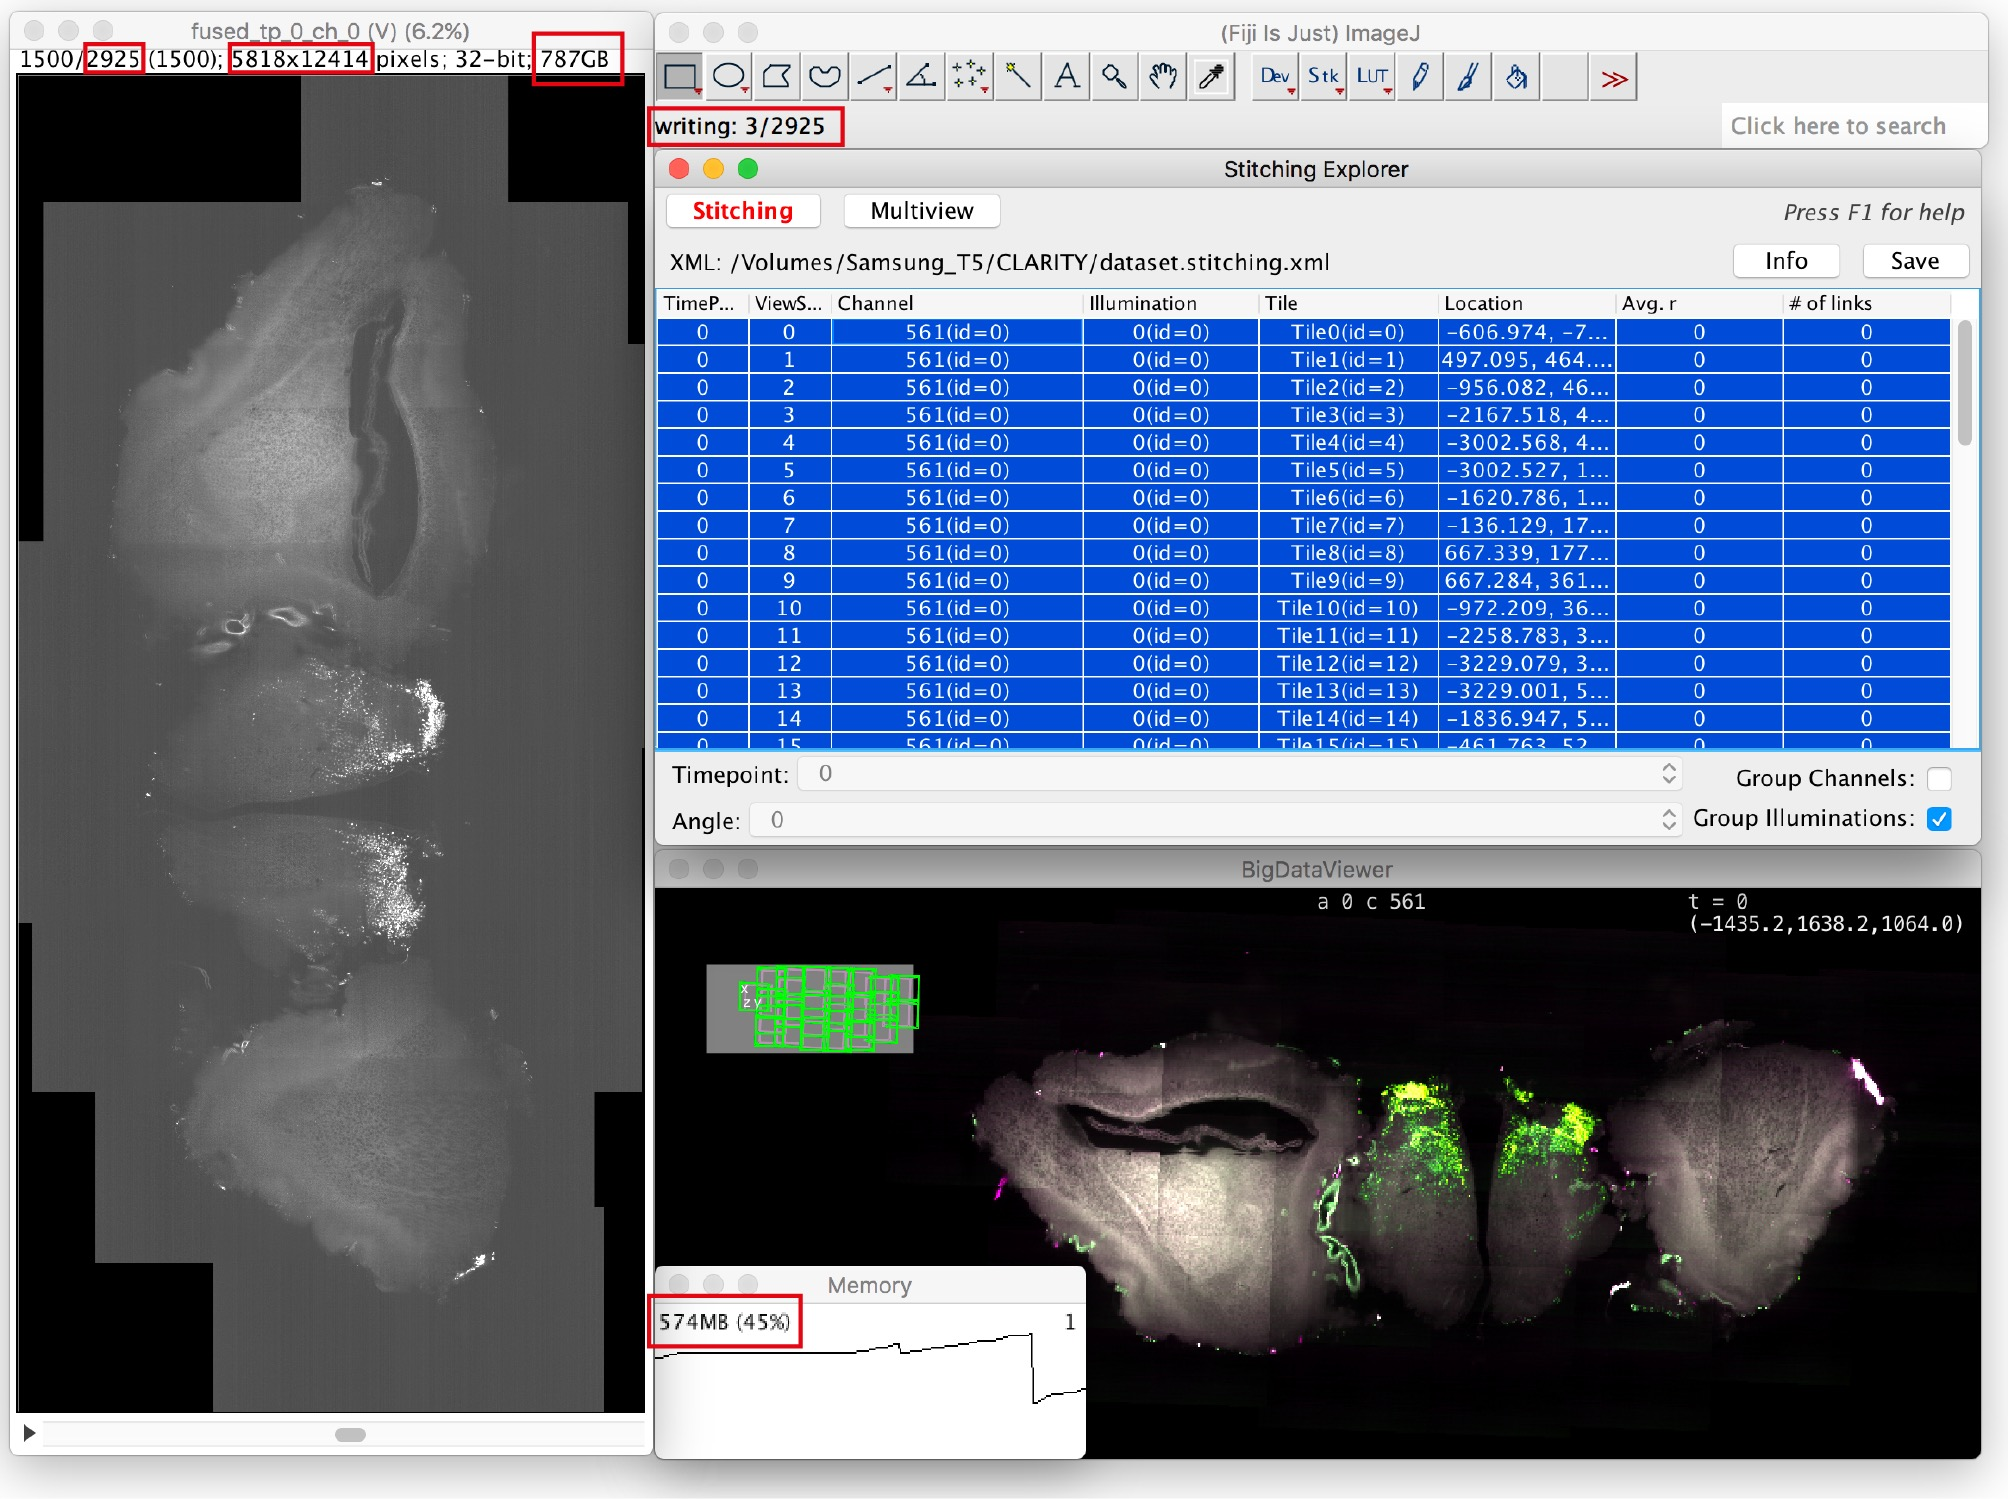
\includegraphics[width=\textwidth]{fig-fusion-screenshot.jpg}
\vspace{-2.0mm}
\caption{\hspace{-0.5mm} \emph{Virtual Fusion.} Screenshot of a Fiji instance running with \textbf{1.25GB of RAM} successfully fusing and saving a \textbf{787GB} volume 5818$\times$12414$\times$2925 pixels in size. This is achieved through \textbf{virtual fusion} combined with virtual, cached loading of blocked, multi-resolution input images. Red boxes highlight memory consumption, size, and progress. During the fusion process, the BigStitcher and BigDataViewer are interactively accessible.
}
\label{fig:sup-fig-fusion}
\end{figure*}

\pagebreak

\subsection*{\red{SUPPLEMENTARY FIGURE 20: Interest point visualization}}
\vspace{1mm}
\begin{figure*}[h!]
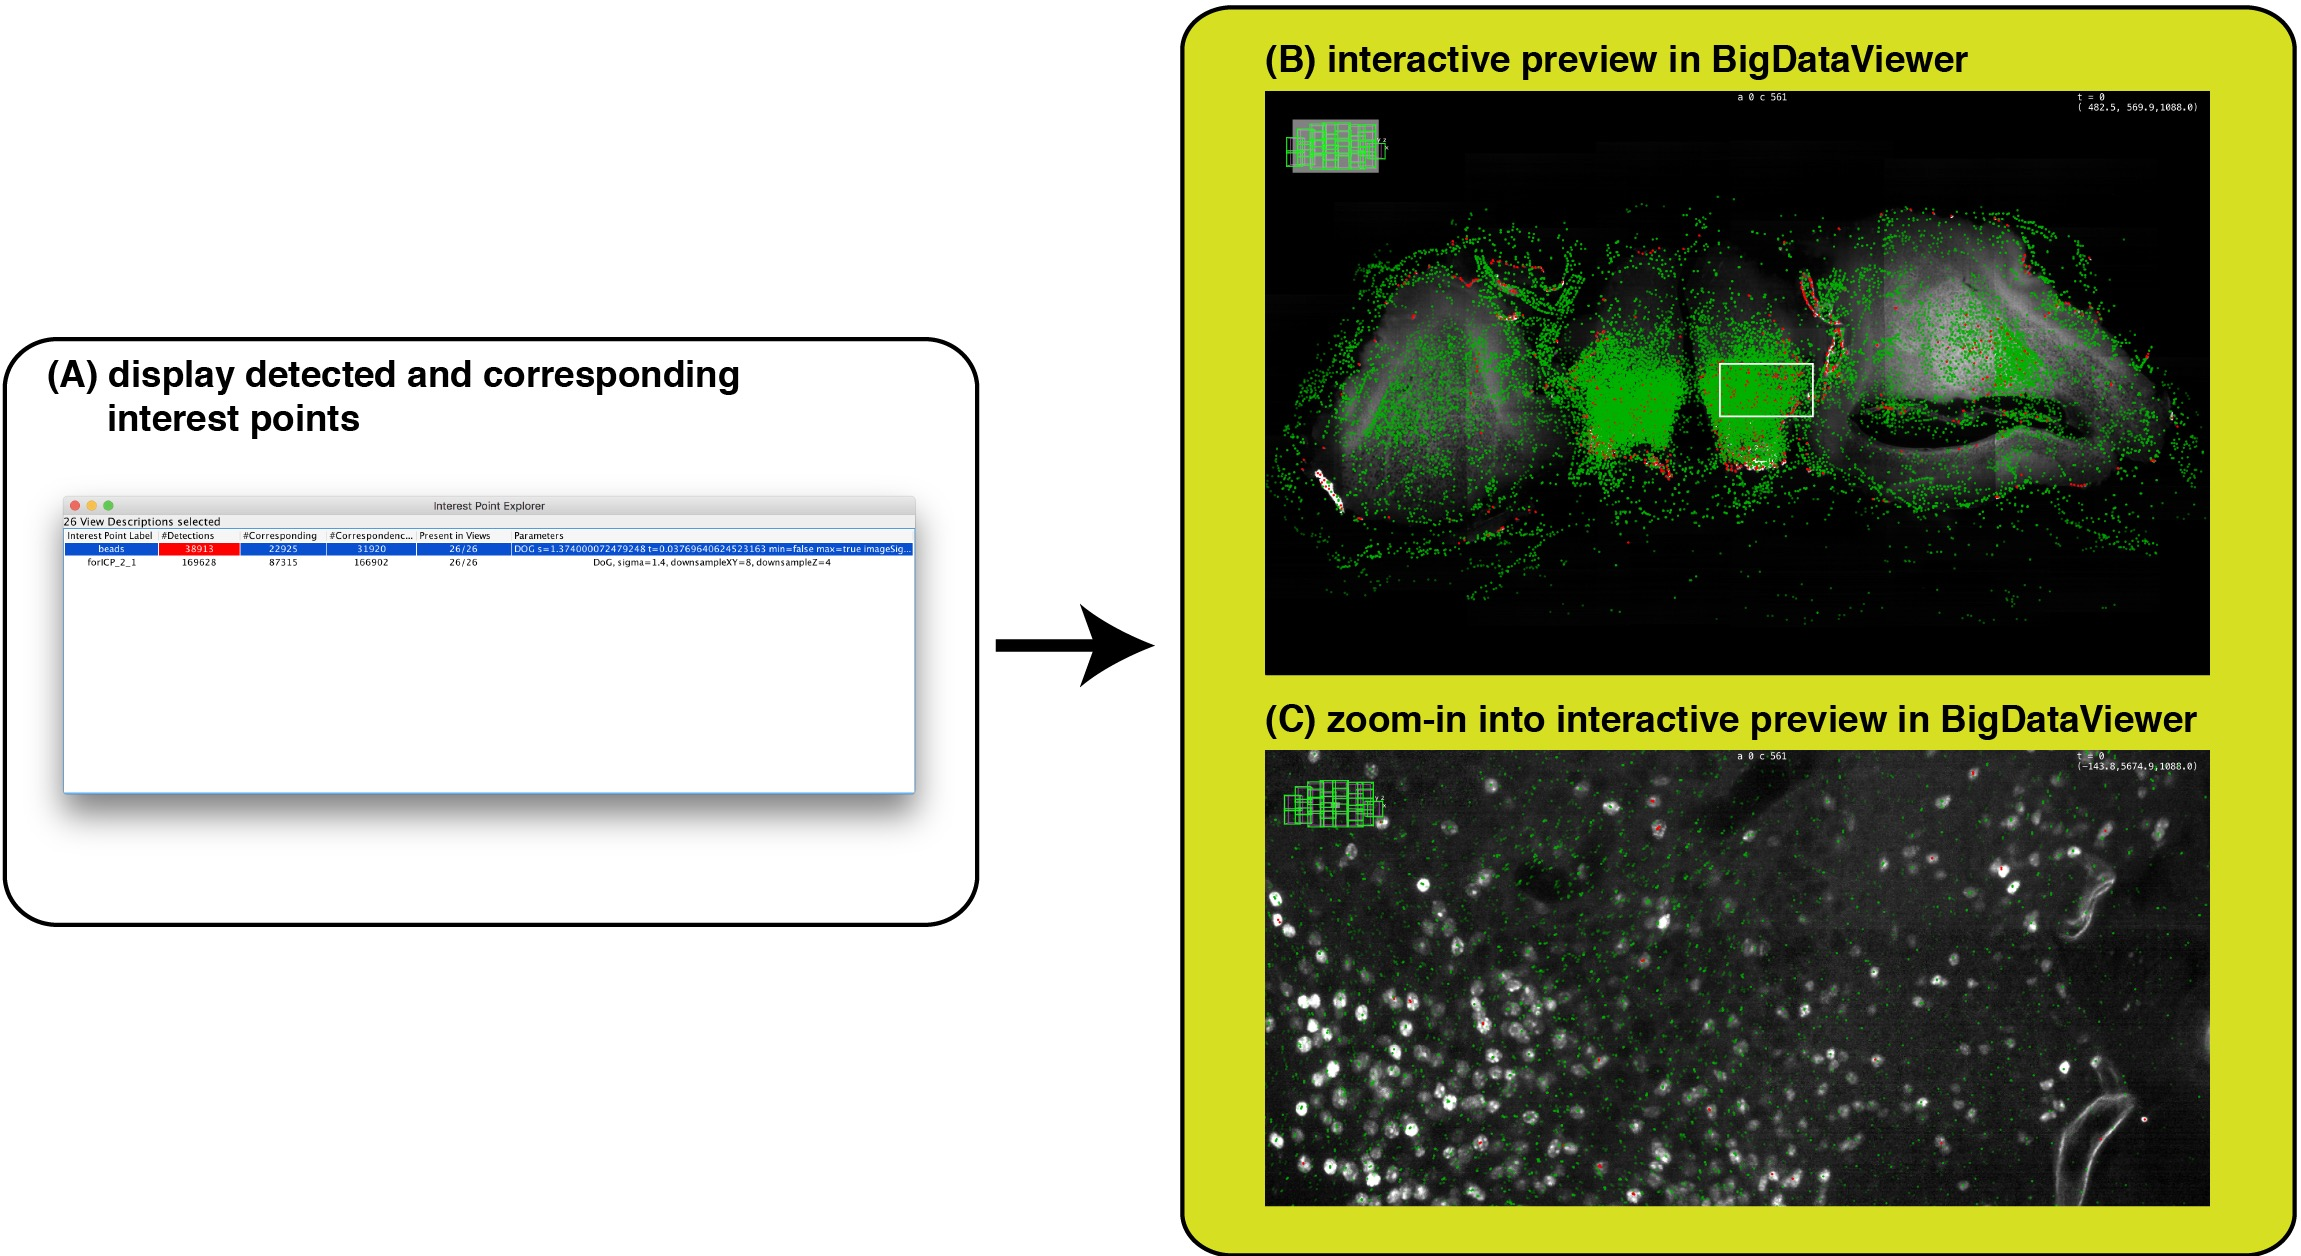
\includegraphics[width=\textwidth]{Supp-IntrestPoints.jpg}
\vspace{-2.0mm}
\caption{\hspace{-0.5mm} \emph{Interactive visualization of interest points.} The interest points explorer allows the visualization of interest points and corresponding interest points between views. \textbf{(A)} select desired interest points for visualization. \textbf{(B)} preview the interest points overlaid in the BigDataViewer. \red{Red dots intersect with the current image plane, green dots are projections from different z-planes. The white box marks the zoom-in shown in (C). \textbf{(C)} Zoom-in into the region outlined in (B).}
}
\label{fig:sup-fig-interest-point}
\end{figure*}

\pagebreak


\subsection*{SUPPLEMENTARY FIGURE 21: Manual transformation of multi-view datasets}
\vspace{1mm}
\begin{figure*}[h!]
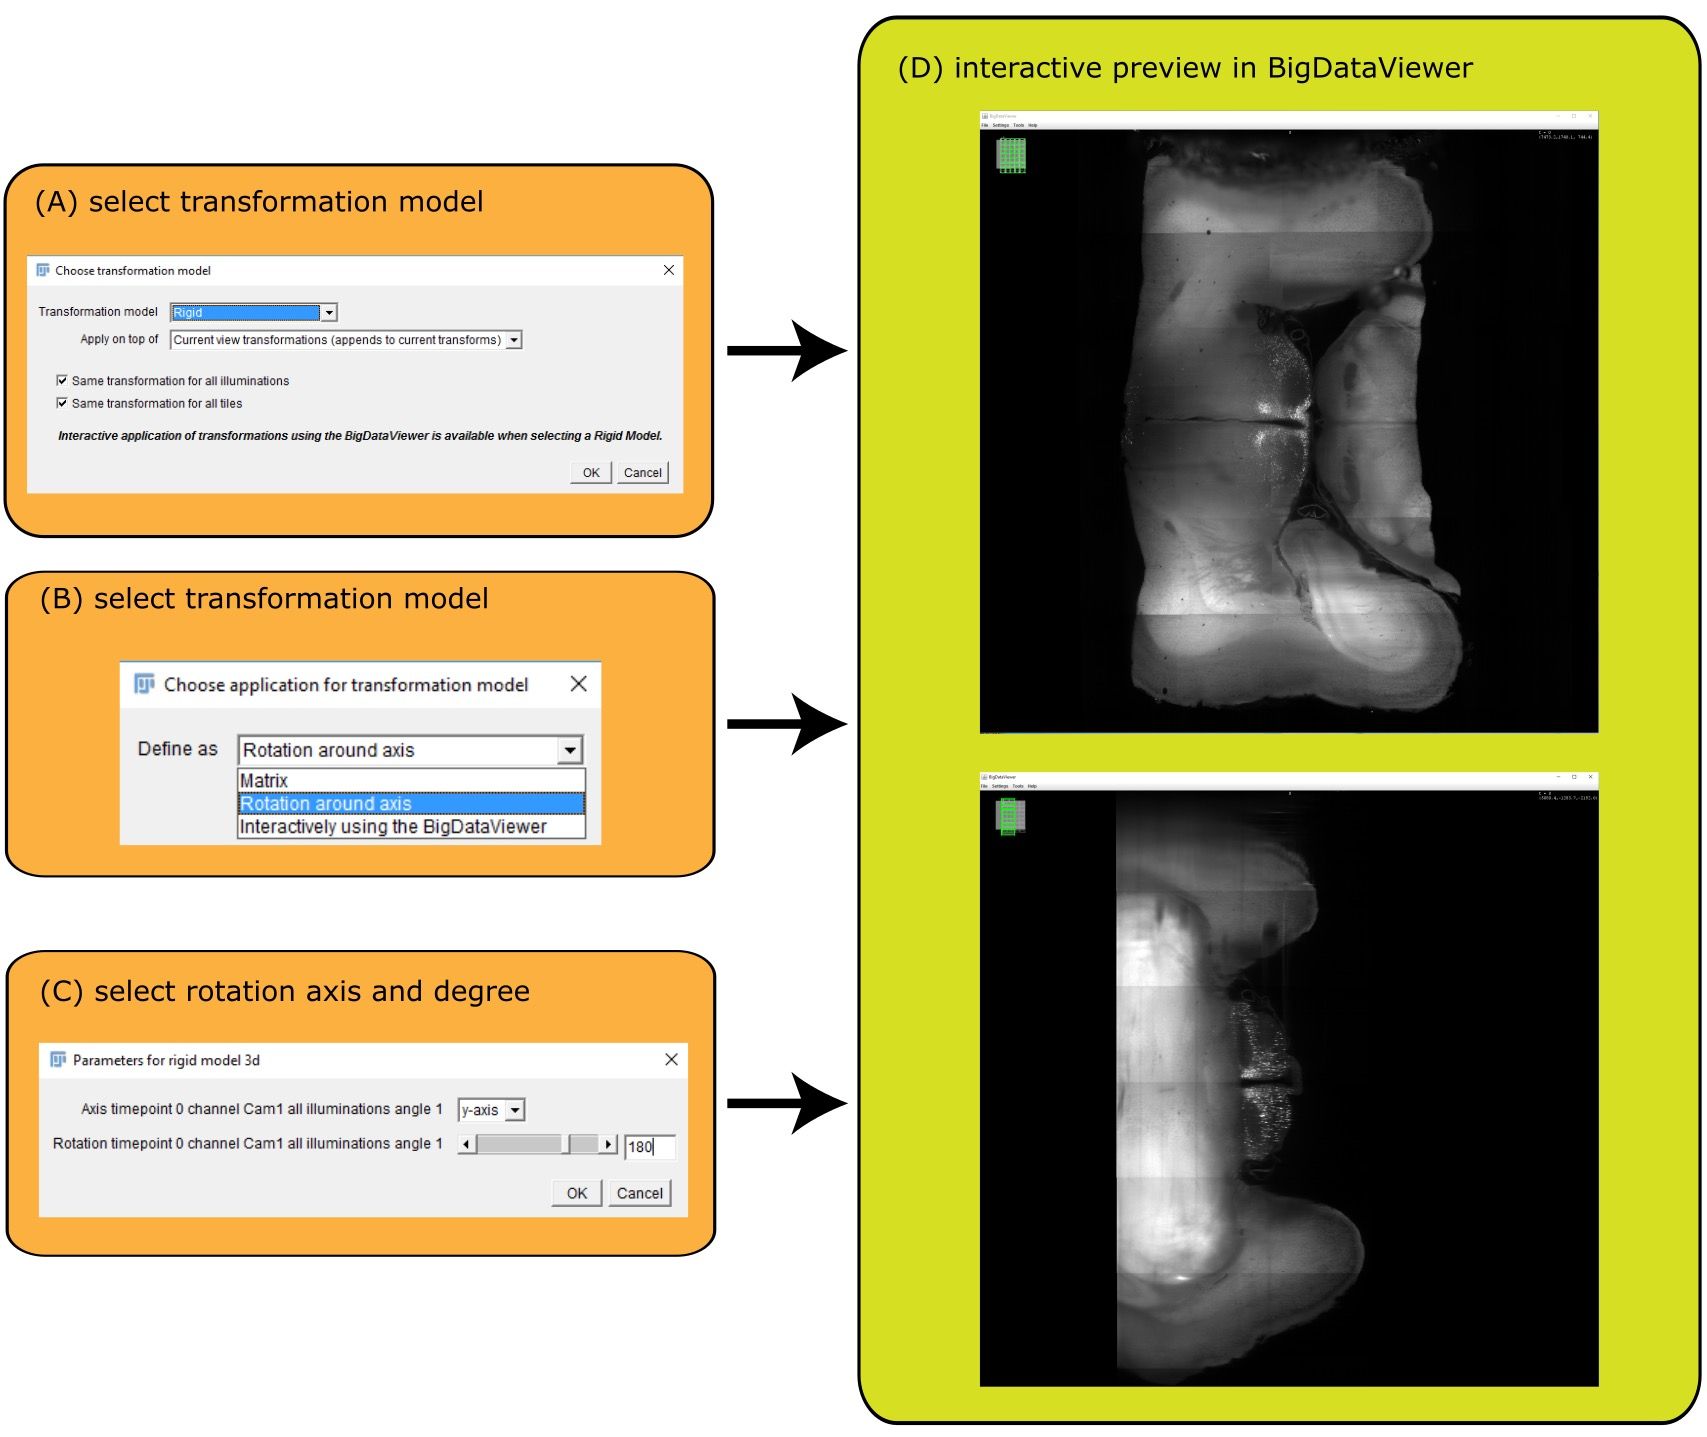
\includegraphics[width=\textwidth]{Supp-Transformation.jpg}
\vspace{-2.0mm}
\caption{\hspace{-0.5mm} \emph{Interactive transformation of views.} Different transformation models can be applied to one or more views and simultaneously visualized in the BigDataViewer. \textbf{(A)} Choose transformation model grouping. \textbf{(B)} Further define the transformation model. In this case a rotation around the axis is selected. \textbf{(C)} Select rotation axis and angle. \textbf{(D)} Visualize rotation of the view in the BigDataViewer.
}
\label{fig:sup-fig-manual-align2}
\end{figure*}

\pagebreak

\subsection*{SUPPLEMENTARY FIGURE 22: Expansion microscopy reconstruction}
\vspace{-2mm}
\begin{figure*}[h!]
\center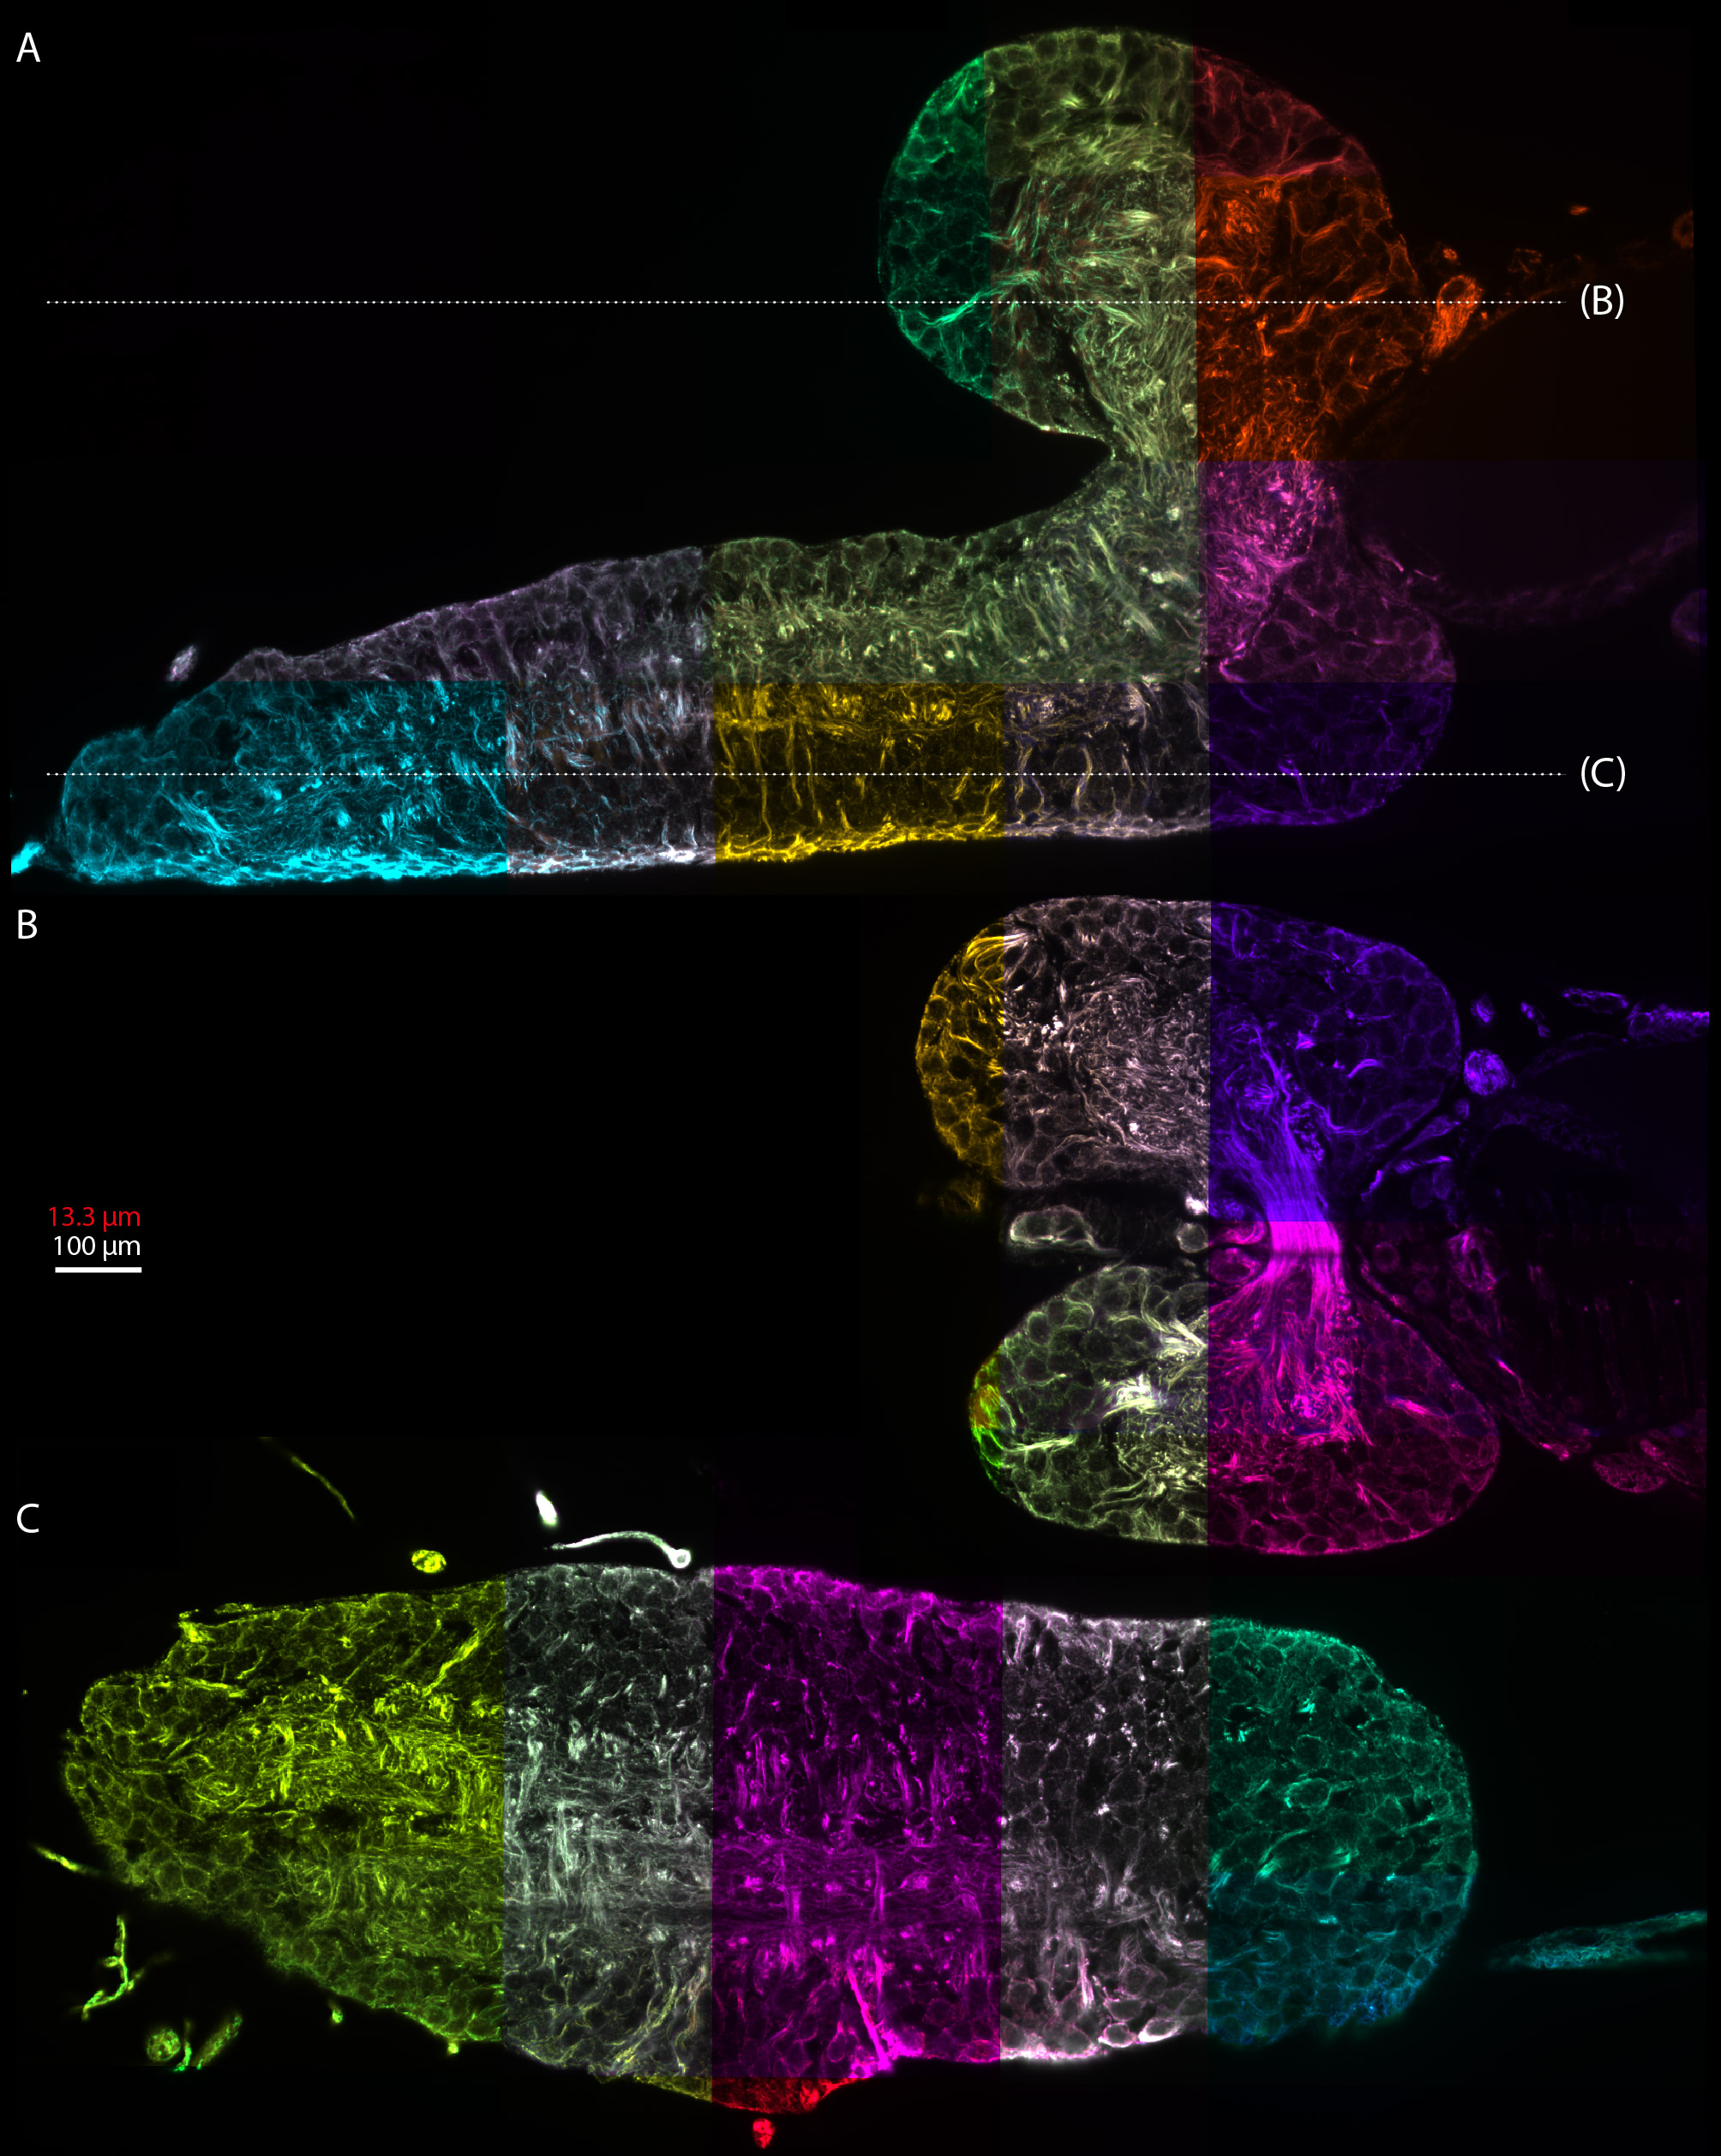
\includegraphics[width=\textwidth-1.9cm]{fig-expansion_tiling.jpg}
\vspace{2.0mm}
\caption{\hspace{-0.5mm} \emph{Expansion microscopy stitching} \red{\textbf{(A)} All tiles (randomly colored) of one view of the expanded Drosophila central nervous system. Dotted lines highlight orthogonal sections in (B) and (C). \textbf{(B,C)} Alignment of an orthogonal view showing at two different cut planes. Red scalebar takes expansion into account. \textbf{(A-C)} Expansion microscopy alignment using phase correlation followed by ICP refinement using affine transformations was performed only on this dataset.}
}
\label{fig:sup-fig-expansion-microscopy}
\end{figure*}

\pagebreak

\subsection*{SUPPLEMENTARY FIGURE 23: Principles of non-rigid alignment}
\vspace{1mm}
\begin{figure*}[h!]
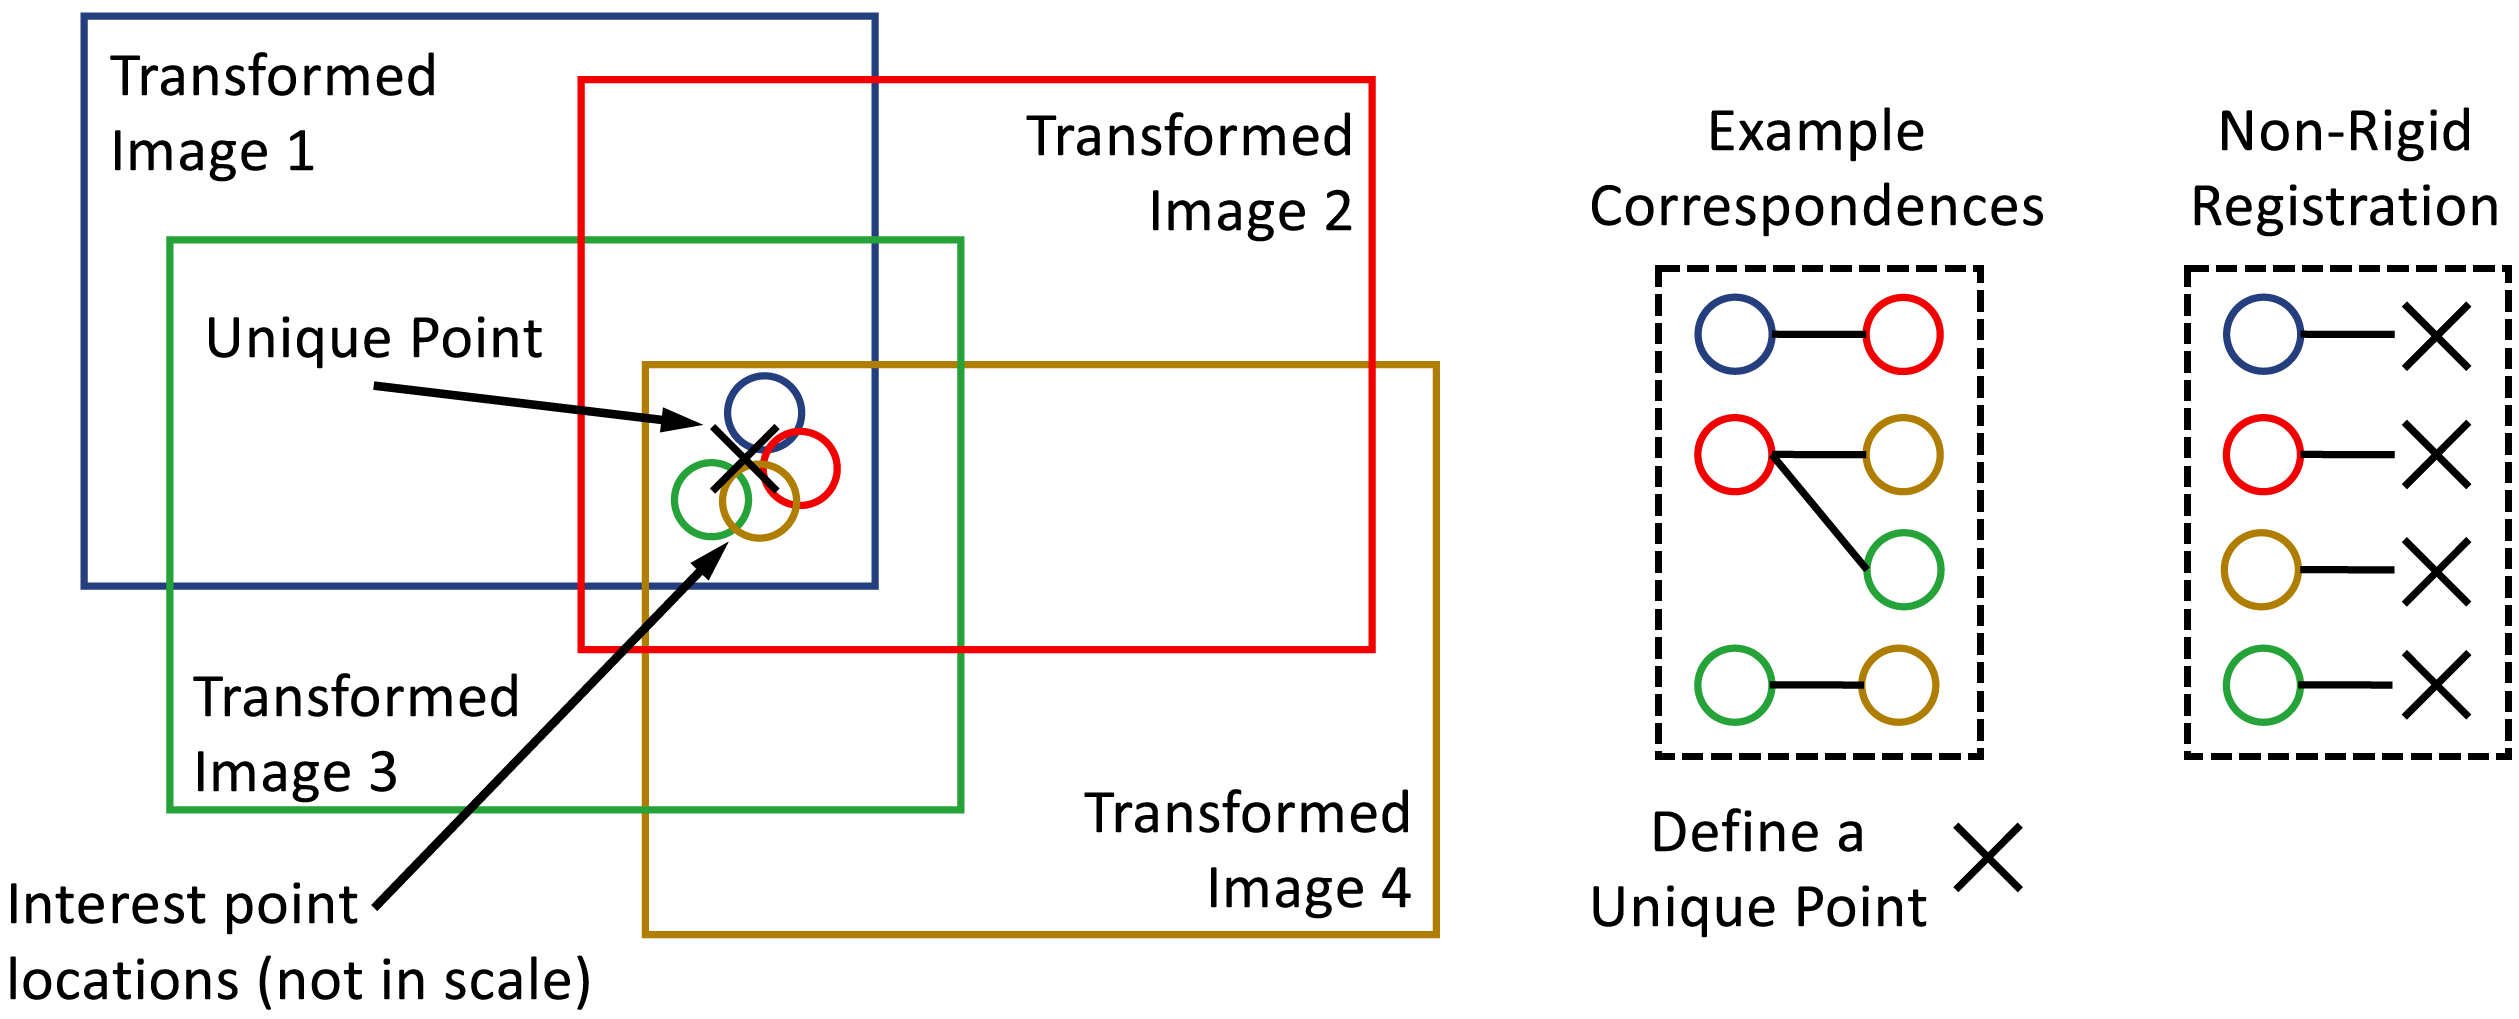
\includegraphics[width=\textwidth]{non-rigid.png}
\vspace{-2.0mm}
\caption{\hspace{-0.5mm} \red{\emph{Principle of Non-Rigid Alignment.} The non-rigid alignment applies a different affine transformation to each pixel of each transformed image. This continuous transformation space is defined by corresponding interest points between overlapping images. We therefore first identify all sets of all corresponding interest points that belong to each other as defined by pairwise correspondences (see Example Correspondences). Each individual set of correspondences across $n$ images then define a $unique$ $point$, of which typically hundreds to thousands per image exist. The left part of the figure illustrates a single $unique$ $point$, which is defined as the average position of all corresponding interest points. Once all unique points are assigned to each correspondence, the non-rigid transformation can be individually computed for each transformed image.
}}
\label{fig:non-rigid}
\end{figure*}

\pagebreak
\begin{landscape}

\setcounter{figure}{1} 
% should be called Supplementary Figure
\renewcommand{\figurename}{Supplementary Table}

\setcounter{table}{0} 

\captionsetup{singlelinecheck = false, format= hang, justification=raggedright, labelsep=space}
  
\fontsize{8.5pt}{10pt}\selectfont
{\color{red}\begin{longtable}{lll}
\caption{\textbf{SUPPLEMENTARY TABLE 1: Summary of all datasets used in this publication}. \label{tab:datasets} }\\ \\

\toprule
\thead[l]{ \textbf{Dataset}} &
\thead[l]{\textbf{Size}} &                                                                                                                                                                                                                                                                                                                                                \thead[l]{\textbf{Microscope \& Acquisition settings}} \\
\midrule \\
\endhead
\midrule
\multicolumn{3}{c}{{Continued on next page}} \\
\midrule
\endfoot

\bottomrule
\endlastfoot
                         \makecell[l]{Coronal slice from a adult \\mouse brain expressing H2B-eGFP\\ under the neuronal BSX promoter\\(\textbf{Figure 3a + Supplement})} &         \makecell[l]{1920$\times$1920$\times$1039 16 bit stacks\\26 tiles from 1 angles (10\% overlap) \\2 channels, single illumination\\\textbf{0.36 TB total size}}  &                                                                     \makecell[l]{Lightsheet Z.1 with EC Plan-Neofluar 5x/0.16 objective, Depth-of-field: $\sim$25$\mu{}m$ \\5.37$\mu{}m$ LS thickness, 538.3647546$\mu{}m$ Confocal parameter\\0.915$\times$0.915$\times$2.57425409$\mu{}m$ pixels\\119.8ms exposure on PCO.edge camera\\lasers: 561 nm 100\%, 488 nm 80\%\\filters: EF1 BP 505-545, EF 2 BP 575-615} \\ \\
                         
                                         \multirowcell{2}[-4ex][l]{Whole adult mouse brain \\expressing H2B-eGFP in all \\BSX-expressing neurons\\(\textbf{Figure 1d-n + Figure 2a,f +}\\ \textbf{Figure 3d,e + Supplement})} &             \makecell[l]{1920$\times$1920$\times$770 16 bit stacks\\56 tiles from 2 angles (10\% overlap) \\2 channels, dual illumination\\\textbf{2.2 TB total size}}  &                                                               \makecell[l]{Lightsheet Z.1 with EC Plan-Neofluar 5x/0.16 objective, Depth-of-field: $\sim$25$\mu{}m$ \\5.97$\mu{}m$ LS thickness, 665.3906758999999$\mu{}m$ Confocal parameter\\0.915$\times$0.915$\times$4.929649351$\mu{}m$ pixels\\119.8ms exposure on PCO.edge camera\\lasers: 561 nm 40\%, 488 nm 40\%\\filters: EF1 BP 505-545, EF 2 BP 575-615} \\ \\
                                                                                                                                   
         &    \makecell[l]{1920$\times$1920$\times$645 16 bit stacks\\63 tiles from 2 angles (10\% overlap) \\2 channels, dual illumination\\\textbf{2.1 TB total size}}  &                                                                    \makecell[l]{Lightsheet Z.1 with EC Plan-Neofluar 5x/0.16 objective, Depth-of-field: $\sim$25$\mu{}m$ \\10.44$\mu{}m$ LS thickness, 2034.834282$\mu{}m$ Confocal parameter\\0.915$\times$0.915$\times$6.203581395$\mu{}m$ pixels\\119.8ms exposure on PCO.edge camera\\lasers: 561 nm 40\%, 488 nm 40\%\\filters: EF1 BP 505-545, EF 2 BP 575-615} \\ \\

 \multirowcell{2}[-4ex][l]{Coronal slice through an adult \\mouse brain expressing an H2B-eGFP \\lineage tracing marker in BSX-expressing \\neurons (\textbf{Figure 3b,e + Supplement})} &            \makecell[l]{1920$\times$1920$\times$828 16 bit stacks\\35 tiles from 2 angles (10\% overlap) \\2 channels, dual illumination\\\textbf{1.55 TB total size}}  &                                                                    \makecell[l]{Lightsheet Z.1 with EC Plan-Neofluar 5x/0.16 objective, Depth-of-field: $\sim$25$\mu{}m$ \\10.44$\mu{}m$ LS thickness, 2034.834282$\mu{}m$ Confocal parameter\\0.915$\times$0.915$\times$4.930096618$\mu{}m$ pixels\\119.8ms exposure on PCO.edge camera\\lasers: 561 nm 50\%, 488 nm 50\%\\filters: EF1 BP 505-545, EF 2 BP 575-615} \\ \\
                                                                                                                                    &             \makecell[l]{1920$\times$1920$\times$960 16 bit stacks\\35 tiles from 2 angles (10\% overlap) \\2 channels, dual illumination\\\textbf{1.8 TB total size}}  &                                                                    \makecell[l]{Lightsheet Z.1 with EC Plan-Neofluar 5x/0.16 objective, Depth-of-field: $\sim$25$\mu{}m$ \\10.44$\mu{}m$ LS thickness, 2034.834282$\mu{}m$ Confocal parameter\\0.915$\times$0.915$\times$4.930916667$\mu{}m$ pixels\\119.8ms exposure on PCO.edge camera\\lasers: 561 nm 50\%, 488 nm 50\%\\filters: EF1 BP 505-545, EF 2 BP 575-615} \\ \\

\makecell[l]{Coronal slice through an adult \\mouse brain expressing an H2B-eGFP \\lineage tracing marker in BSX-expressing \\neurons  (zoomed-out) \\(\textbf{Figure 2k-m + Supplement})} &  \makecell[l]{1920$\times$1920$\times$945 16 bit stacks\\12 tiles from 2 angles (10\% overlap) \\1 channel, dual illumination\\\textbf{0.166 TB total size}}  &  \makecell[l]{Lightsheet Z.1 with EC Plan-Neofluar 5x/0.16 objective (0.5$\times$ zoom) \\ Depth-of-field: $\sim$35$\mu{}m$\\ 10.44$\mu{}m$ LS thickness, 2034.834282$\mu{}m$ Confocal parameter\\1.83$\times$1.83$\times$4.93$\mu{}m$ pixels\\119.8ms exposure on PCO.edge camera\\lasers: 488 nm 50\%\\filters: EF1 BP 505-545} \\ \\

                              \makecell[l]{Whole \emph{C. elegans} during dauer \\with all neuron nuclei expressing tagRFP in \\and co-stained with DAPI (\textbf{Figure 3e,f})} &  \makecell[l]{750$\times$1920$\times$40 16 bit stacks\\16 tiles from 4 angles (10\% overlap) \\2 channels, single illumination\\\textbf{0.003 (2,96GB) TB total size}}  &  \makecell[l]{Lightsheet Z.1 with W Plan-Apochromat 20x/1.0 objective (2$\times$ zoom)\\ Depth-of-field: $\sim$1$\mu{}m$\\1.82$\mu{}m$ LS thickness, 56.72238239$\mu{}m$ Confocal parameter\\0.114$\times$0.114$\times$0.8035$\mu{}m$ pixels\\59.9ms exposure on PCO.edge camera\\lasers: DAPI 505 nm 2\%, DAPI 561 nm 0.2\%, RFP 561 nm 5\%\\filters: DAPI CAM BS Mirror, RFP CAM BS SBS LP 560, RFP EF 1 BP 575-615} \\ \\
                          \makecell[l]{Central nervous system of a Drosophila\\ 1st instar larva with immunostaining \\for tubulin (\textbf{Figure 3c,e + Supplement})} &                     \makecell[l]{2048$\times$2048$\times$923 stacks\\26 tiles from 2 angles (28\% overlap) \\1 channels, dual illumination\\\textbf{0.188 TB total size}}  &                                                                                                                \makecell[l]{IsoView with SpecialOptics 16x/NA 0.71 objective\\ Depth-of-field: $\sim$2$\mu{}m$ \\4.92$\mu{}m$ LS thickness, 416.0$\mu{}m$ Confocal parameter\\0.4125$\times$0.4125$\times$0.8125$\mu{}m$ pixels\\20.1ms exposure on Orca Flash 4.0 v2 sCMOS camera\\lasers: 488 nm 10.6mW\\filters: BP488/10 EX, BP525/50 EM } \\ \\

\caption{\red{\emph{Note: Depth-of-field was estimated based on the descriptions on this resource \href{https://www.microscopyu.com/microscopy-basics/depth-of-field-and-depth-of-focus}{Depth of Field and Depth of Focus | MicroscopyU}.}}}

\end{longtable}}

\pagebreak

\captionsetup{singlelinecheck = false, format=plain, justification=justified, labelsep=space}

\subsection*{SUPPLEMENTARY TABLE 2: Performance comparison}
\vspace{-3mm}
\begin{figure*}[h!]
\center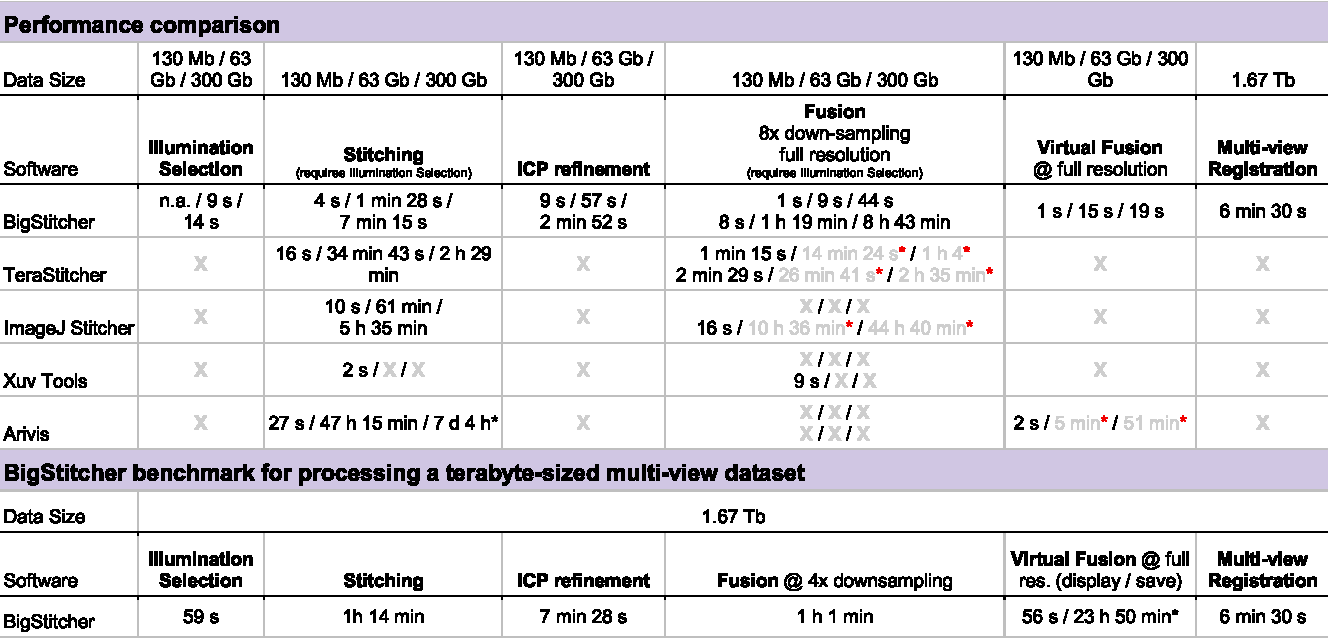
\includegraphics[width=\textwidth+5.00cm]{supp_table_1.pdf}
\vspace{-3mm}
\caption{\hspace{-0.5mm} \red{\emph{Comparison of BigSticher features and performance with other available stitching programs for four different datasets with different sizes (130 Mb, 63 Gb, 300 Gb, and 1,67 Tb).} Benchmarks were performed on a HP Z840 workstation running Windows 10 Pro with two Intel Xenon E5-2667v4 CPUs and 512 GB memory. The benchmarks for the Arivis software were performed on a HIVE system running Windows Server 2012 R2 with two Intel Xenon E5-2640v3 CPUs and 256 GB memory. The latest stable version of each stitching program was used. BigStitcher datasets were stitched using 4$\times$ times (x,y) downsampling, and fusion was performed at stated downsampling levels. Correctness of the stitching could only be confirmed in the BigStitcher due to the flexibility of interactive inspection. Processing of multi-view, dual-illumination datasets as well as ICP refinement and virtual fusion is only possible in BigStitcher. Note that fusion in BigStitcher also performs intensity adjustment. All displayed values are averaged from three independent runs of each respective software except those marked with a black star. \textbf{Note that image fusion results are not comparable since all other applications fuse datasets using translation-only, which is a significantly simpler problem that cannot align the datasets sufficiently well while BigStitcher uses affine models. Therefore translation-only results on dual-illumination datasets are grayed and marked with a red star.} A cross indicates that the functionality is not supported by the software, 'n.a.' indicates that the dataset did not require this feature.}
}
\label{tab:benchmarks}
\end{figure*}

\end{landscape}
\pagebreak



\input supplementary-methods.tex

%\pagebreak
%\titleformat{\section}{\centering\normalfont\fontsize{13.5pt}{1em}\bfseries}{SUPPLEMENTARY NOTE \thesection: }{0em}{}
\section{BigStitcher user guide}
\label{sec:documentation}

\subsection{This is where the documentation will go}

Lorem ipsum dolor sit amet.

%\pagebreak

\section{Example datasets for BigStitcher}
\label{sec:example}

We prepared three different examples of different size and complexity for testing the BigStitcher. We suggest to run BigStitcher on these first before applying it to your dataset. This allows you to quickly test features in an environment where you can easily ask for advice on GitHub or the ImageJ Forum.

\textcolor{red}{The data can be downloaded from the Open Science Foundation (a Nature recommended data repository \url{https://www.nature.com/sdata/policies/repositories}) at \url{https://osf.io/bufza/}.}

\begin{description}
\item 2d multi-tile dataset ($2.8$ MB) \\
Maximum intensity projection of the nervous system of a Drosophila larva containing 6 tiles and 3 channels each. You can download the raw input at \url{http://preibischlab.mdc-berlin.de/BigStitcher/Grid_2d.zip} and a reconstructed BigStitcher project at \url{http://preibischlab.mdc-berlin.de/BigStitcher/Grid_2d_h5_aligned.zip}. In the reconstructed project, the images were imported into the BigStitcher using the AutoLoader (with immediate resaving as HDF5 and Movement to a regular 2-by-3 grid with 10\% overlap between the tiles). We calculated pairwise shifts using phase correlation with default parameters, using the precomputed 2x2 downsampling and averaging the channels. We ignored links with correlation $<0.7$ and calculated the final registration using the two-round global optimization with strict constraints. 
\item 3d multi-tile dataset ($123$ MB)
\begin{sloppypar} % to prevent ugly linebreak in url
3d confocal scan of the nervous system of a Drosophila larva containing 6 tiles and 3 channels each, channels are distributed over different files. You can download the raw input at \url{http://preibischlab.mdc-berlin.de/BigStitcher/Grid_3d.zip} and the reconstructed project at \url{http://preibischlab.mdc-berlin.de/BigStitcher/Grid_3d_h5_aligned.zip}. In the reconstructed project, we ran the same import and reconstruction steps as for the 2d dataset and in addition performed affine refinement of the registration using IPC with default parameters and simple tile refinement to create the final reconstructed project.
\end{sloppypar}
%\item 3d multi-tile multi-view dataset ($12$ GB)\\ 
%3d light-sheet scan of a cleared section of an adult mouse brain expressing H2B-GFP in all bsx neurons. It contains 2 orthogonal angles, 2 illumination directions, and 6 tiles. It was downsampled 2-fold in each dimension from its original size. You can download the \textbf{raw} BigStitcher project in HDF5 format where tiles are placed according to the approximate coordinates from the microscope at \url{http://preibischlab.mdc-berlin.de/BigStitcher/Clearing_3d_h5.zip}. You can download the XML file describing the \textbf{fully reconstructed} dataset (works with the same HDF5 file) at \url{http://preibischlab.mdc-berlin.de/BigStitcher/Clearing_3d_xml_aligned.zip}. You simply need to extract this small $1.5$~MB archive into the same directory as the .h5 file and open the xml file in BigStitcher. In order to reconstruct the sample, we performed the following steps:
%\begin{itemize}
%\item Illumination Selection (Pick Brightest)
%\item For each angle:
%	\begin{itemize}
%		\item Select all views, Stitch dataset with downsampling 4,4,2
%		\item Correlation range $0.7$ ... $1.0$, filter z-shift by $25$ pixels, global optimization with RELAXED handling
%		\item Refine with ICP, simple (tile registration)
%	\end{itemize}
%\item Switch to multi-view mode, select 2nd view only, apply transformation, same for all, rotation around axis, $180$ degrees around the Y-axis
%\item Select both, register using interested points, fast translation invariant, compare all views, forICP\_2\_1, group tiles and illuminations, fix first view, do not map back, affine, regularize, redundancy $1$, significance $1.5$, RANSAC error $30$, iterations VERY THOROUGH, regularize with rigid, lambda $0.1$, simply group, merge distance $5$.
%\item Select both, detect interest points, Difference-of-Gaussian, label nuclei, group tiles and illuminations, 3-d quadratic fit, interactive, downsample XY $4$, downsample Z $2$, same min and max for all, in interactive or advanced mode sigma=$1.3645$ and threshold=$0.008432$
%\item Select both, register using interested points, assign closest-points, only overlapping views, label nuclei, do not group, affine, regularize, max distance $5$, max iterations $100$, regularize with rigid, lambda $0.1$
%\item Fuse as desired ...
%\end{itemize}
\end{description}

We will add larger and more complex examples on the BigStitcher website \url{https://imagej.net/BigStitcher} and will also link videos of the  alignment process from there.

%\pagebreak

% description of current version location is in currentcode.tex 
\input currentcode.tex


%\section{OTHER RELATED LITERATURE}
%The field of multi-view deconvolution is large and diverse; many areas of science contribute including medical science, astronomy, microscopy and the classical computer science. Within the focus of this publications it is not possible to discuss all aspects (e.g. multi-channel deconvolution). We therefore list other publications that contributed to various aspects of multi-image deconvolution\cite{Rajagopalan1998, Giannakis2000, Flusser2003, Vieilleville2011, heintzmann2002, ShawAl89,agard1984,agard1989,verveer1998,heintzmann2000,holmes1991,blume2007}.


%%%%%%%%%%%%%%%%%%%%%%%%%%%%%%%%%%%%%%%%%%%%%%%%%%%%%%%%%%%%%
%\acknowledgments     %>>>> equivalent to \section*{ACKNOWLEDGMENTS}

%%%%%%%%%%%%%%%%%%%%%%%%%%%%%%%%%%%%%%%%%%%%%%%%%%%%%%%%%%%%%
%%%%% References %%%%%

\bibliography{supplement-bibliography}   %>>>> bibliography data in supplement-bibliography.bib
\bibliographystyle{spiebib}   %>>>> makes bibtex use spiebib.bst

\end{document}
